\documentclass[12pt, a4paper]{report}
\usepackage[a4paper, total={6in, 8.9in}]{geometry}
\usepackage{titlesec}
\usepackage{graphicx}
\usepackage{subfig}
\usepackage[parfill]{parskip}
\usepackage{amsmath} %Used to change formulas names
\graphicspath{ {images/} }
\usepackage{pgfplots}
\usepackage{filecontents}
\usepackage{hyperref}
\usepackage{listings}
\usepackage{nomencl}
\usepackage{mathtools} 
\usepackage[style=numeric]{biblatex}
\usepackage{enumerate}
\usepackage{multirow}
\usepackage{tabularx}
\usepackage{nomencl}
\makenomenclature
\usepackage[toc,page]{appendix}
\usepackage{color, colortbl}
\usepackage{pifont}
\usepackage{float}
\usepackage{listings}
\usepackage{xcolor}
\usepackage{pdfpages}

\definecolor{codegreen}{rgb}{0,0.6,0}
\definecolor{codegray}{rgb}{0.5,0.5,0.5}
\definecolor{codepurple}{rgb}{0.58,0,0.82}
\definecolor{backcolour}{rgb}{0.95,0.95,0.92}


\lstdefinestyle{Python}{%
    backgroundcolor=\color{backcolour},   
    commentstyle=\color{codegreen},
    keywordstyle=\color{magenta},
    numberstyle=\tiny\color{codegray},
    stringstyle=\color{codepurple},
    basicstyle=\ttfamily\footnotesize,
    breakatwhitespace=false,         
    breaklines=true,                 
    captionpos=b,                    
    keepspaces=true,                 
    numbers=left,                    
    numbersep=5pt,                  
    showspaces=false,                
    showstringspaces=false,
    showtabs=false,                  
    tabsize=2,
    columns=fullflexible,
    keepspaces=true,
    upquote=true,
    language=Python, % <=====================================================
}

\lstdefinestyle{Cplus}{%
    backgroundcolor=\color{backcolour},   
    commentstyle=\color{codegreen},
    keywordstyle=\color{magenta},
    numberstyle=\tiny\color{codegray},
    stringstyle=\color{codepurple},
    basicstyle=\ttfamily\footnotesize,
    breakatwhitespace=false,         
    breaklines=true,                 
    captionpos=b,                    
    keepspaces=true,                 
    numbers=left,                    
    numbersep=5pt,                  
    showspaces=false,                
    showstringspaces=false,
    showtabs=false,                  
    tabsize=2,
    columns=fullflexible,
    keepspaces=true,
    upquote=true,
    language=C++, 
}

\addbibresource{References.bib}

%% --------------------------- Begin Document ------------------------%
\begin{document}

%% ------------------ Cover Letter ------------------ %

\begin{titlepage}
\center % Center everything on the page

\includegraphics[scale=0.8]{logo/CranfieldUniLogo.png}\\[1.5cm]
\textsc{\LARGE Cranfield University}\\[0.3cm] 
\textsc{School of Aerospace, Transport and Manufacturing}\\[3cm]
\textsc{\Large Thesis Project}\\ [0.3cm]
{ \Large \bfseries Analysing Expected Goals (xG) in Football}\\[0.3cm] % 
\textsc{ MSc. Computational and Software Techniques in Engineering}\\[3cm]
\emph{Authors:}\\[0.1cm]

Ayush Maria - s349256\\[0.5cm]

\emph{Module Supervisor:}\\ [0.1cm]

Dr. Jun Li \\[1cm]


\textbf{Revised edition, 2026}\\[0.2cm]
Original edition submitted August 2022\\ [0.4cm]

%\vfill % Fill the rest of the page with whitespace
\end{titlepage}

% ---------------- parameters for margins spaces --------------------%
\titleformat{\chapter}[display]   
{\normalfont\huge\bfseries}{\chaptertitlename\ \thechapter}{20pt}{\Huge}   
\titlespacing*{\chapter}{0pt}{-55pt}{40pt}
\titleformat{\chapter}[display]
{\normalfont\bfseries}{}{0pt}{\Huge}

% ------------------- Table of contents ----------------------------%
\tableofcontents
\listoffigures
\listoftables

%% ---------------------------- Acronyms ----------------------------%
\nomenclature{\(xG\)}{Expected Goals}
\printnomenclature



%% --------------------------- Abstract -----------------------------%
\begin{abstract}
Data science and statistics are now part of how football clubs analyse players and teams, recruit in the transfer market and plan for matches. Expected Goals (xG), the probability that a shot results in a goal given the situation it was taken in, is one of the central metrics of this work. This study builds xG models from StatsBomb's open event data: 61,003 open-play shots from 2,616 men's matches since 2000, across the four major European leagues, international tournaments and other competitions. Thirteen features describe each shot, including the positions of the defenders and the goalkeeper taken from StatsBomb's freeze frames. Four algorithms (Logistic Regression, XGBoost, LightGBM and CatBoost) were tuned by cross-validation and tested on 524 held-out matches. All four are well calibrated, predicting within 1.5\% of the goals actually scored, and they are almost tied (AUC 0.804--0.806); the features describing the shot matter far more than the algorithm. The models are then used to analyse teams and players: xG difference tracks the 2015/16 league tables closely, Leicester City won the Premier League while ranking 6th on xG difference, and Lionel Messi scored almost 99 more open-play goals than his chances were worth. Finally, a model pooled across the Premier League, La Liga, Serie A and Ligue 1 is shown to be calibrated in each of them, and more accurate than separate models per league.
\end{abstract}

%% --------------------------- Preface ------------------------------%
\chapter*{Preface to the Revised Edition}
\addcontentsline{toc}{chapter}{Preface to the Revised Edition}
The original edition of this thesis was submitted in 2022. Its models were trained on the 520 La Liga matches then available in StatsBomb's open data, all of which involved FC Barcelona, so its results described one exceptional team rather than football in general. This revised edition repeats the study on all men's matches in the open data, with the following changes:
\begin{itemize}
    \item \textbf{Data:} 61,003 open-play shots from 2,616 men's matches since 2000, instead of the shots of one club. Two errors in the data preparation were also corrected: the goalkeeper's position is now reset for every shot, and shots are assigned to teams through the match line-ups.
    \item \textbf{Exploratory analysis:} every figure has been redrawn on the new data, using the training matches only, and every statement has been checked against it. Where a feature's relation with goals depends on shot distance, it is now compared within distance bands. Some conclusions changed as a result, for example on kick-offs and on pass type.
    \item \textbf{Evaluation:} the data is split by match rather than by shot, the models are tuned by cross-validated log loss, and calibration is reported alongside AUC.
    \item \textbf{Results:} feature importance, team and player analysis are based on the new models and on out-of-fold predictions, and a new section tests whether one model can serve several leagues.
\end{itemize}
The introduction and literature review are unchanged apart from minor edits. All numbers and figures can be reproduced with the code in the project repository (section \ref{sec:revised-pipeline}).


%%--concrete steps in the past t--------------- links to all sub-documents ---------------------%

\chapter{Introduction}\label{football}
Football is one of the most well-known athletic activities in the world \cite{giulianotti2012football}. People affiliated with football clubs and teams, as well as fans , are occasionally faced with scenarios in which it is impossible to predict how the teams perform in critical junctures. This acts as the source of cognitive bias, outcome bias, and the all-important "availability heuristic" within these people's perceptions. \cite{biermann2019football}

Anticipating football match results may be a valuable technique for judging a club's or team's preparedness before a game. Though forecasting  sounds like a deal maker, it could be in the betting industry. This is due to the fact that football is governed by chance. \cite{biermann2019football} Forecasts may be impacted not only by significant elements such as possession, amount of shoots, precision in the final third, and so on, but also by weather, turf conditions, player mindset, the number of fans present in the game, and a plethora of others. Such criteria can quickly reveal the underlying cause of any specific team's performance. To better react to the scenario, teams must use and adopt different plans during the game. The goal of this research project is to create a framework that analyses an essential statistic in football that centres around the chance of a football shooting chance from a specific location, hence improving football strategy. 

Expected Goals (xG) is the name of this measure. It may be influenced by a plethora of variables, such as the range from the goal, whether it was shot with a stronger foot, the number of people surrounding the shooter and the goal, the shot angle, the build-up play to the goal, and more. Expected Goals is essential for determining player profiles, transfer market trends, and club tactics. This statistic has been used by several clubs and teams, including Liverpool F.C., and has assisted them in winning championships like the Premier League and the UEFA Champions League. Luis Diaz, who was bought by Liverpool F.C. in January and has already helped the team reach its second Champion's League final in three years, is the most notable example of a player Liverpool F.C. has profiled in the transfer window. \cite{lichtenthaler2020mixing}

\section{Aims and Objectives}

\begin{itemize}
    \item Measure the quality of chances created by footballers and footballing teams
    \item Highlight the use of Expected Goals (xG) in player profiling and match strategy
    \item Introduce how AI based on Probability is used in football 
    \item Establish a bedrock for future metrics 
    \item Test whether one xG model can serve different leagues and styles of play
\end{itemize}



\chapter{Literature Review}\label{lit}
Numerous sports, like basketball \cite{skinner2010price} and baseball \cite{albert2010baseball}, have made use of artificial intelligence to glean insights from data and adjust their tactics. On the other hand, because it is a closed sector, football has only lately witnessed the integration of such technologies within its systems.
Data was previously ignored in this sport since the hierarchies are driven by professionals like former players and scouts. \cite{kuper2018soccernomics}

A plethora of studies attempted to forecast football match results by taking into account characteristics of the tournaments or leagues these matches were organized in. Although initially promising, as shown in some of the publications mentioned below, this strategy does not aid football teams in formulating plans during live matches.
Here are some examples of publications that explore this topic: 
\begin{itemize}
    \item Authors \citeauthor{5596458} \cite{5596458} stated that their study used an Artificial Neural Network to the dataset from the 2006 FIFA World Cup and claimed that if the drawn matches are not taken into account, an accuracy of 76.9\% may be attained. This investigation established a standard for football statistics. It is essential to remember that every football tournament is unique, and training a model for every competition is not creative. 
    \item Authors \citeauthor{joseph2006predicting} \cite{joseph2006predicting} study aims to predict game outcomes for the Tottenham Hotspur football team. In addition to Decision Tree algorithm and the K-nearest neighbours method, a Bayesian network was used in the implementation. The Bayesian Network fared better than other algorithms in terms of prediction accuracy in this domain, according to the authors' research. The study's overall accuracy came at 59.21\%. (win, draw or lose). 
    \item  Genetic programming was used by \citeauthor{6604116} \cite{6604116} to predict the outcomes of English Premier League games, which may end in a win, loss, or a tie. As an input to the Genetic Program system, they selected 25 traits from each game, and the system then created a function to predict the result. A single GP-generated function's prediction accuracy underwent an experimental test, and the results looked good. For each League game played for each season, this study manually fed 25 different characteristics. The shortcomings of forecasting football games are shown by this as well as the fact that the resultant accuracy was 70\%. 
    \item To find non-linear correlations, authors \citeauthor{rotshtein2005football} \cite{rotshtein2005football} created a model that uses fuzzy logic as the foundation. To fine-tune fuzzy rules and get acceptable simulation results, they used competition data. The tuning method involved determining the parameters of the fuzzy membership functions and rule weights using a combination of genetic and neural optimization approaches. The model is promising, but it does not take into account variables like injured players, players who have been booked and benched, referee prejudice, and weather conditions. Additionally, owing to its nature, it only forecasts results based on previous matches. 
\end{itemize}

These publications made it simple to understand how football match prediction models take into account variables that have nothing to do with the tactics used, but rather with the patterns and results of earlier games. This went against the objective of the case study. 

\begin{figure}[!h]
    \centering
    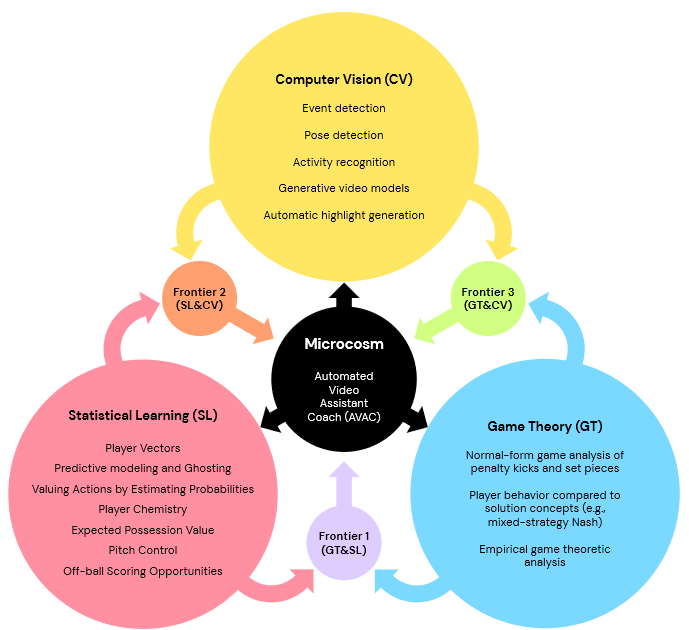
\includegraphics[scale=0.75]{images/deepmind.PNG}
    \caption{Proposed model by deepmind}
    \label{fig:my_label}
    \cite{DBLP:journals/corr/abs-2011-09192}
\end{figure}

The study carried out by DeepMind Technologies, a division of Alphabet Inc. \cite{DBLP:journals/corr/abs-2011-09192}, illustrates the present impact of several branches of artificial intelligence on football analytics. As shown in the graphic  \ref{fig:my_label}, statistical learning, computer vision, and game theory work together to produce a possible system for football analytics that has the potential to spark a data revolution.

This case study sought to demonstrate statistical learning using the Expected Goal (xG) measure, which Vic Barnett and Sarah Hilditch initially introduced in their 1993 publication. \cite{barnett1993effect}

\begin{figure}[!h]
    \centering
    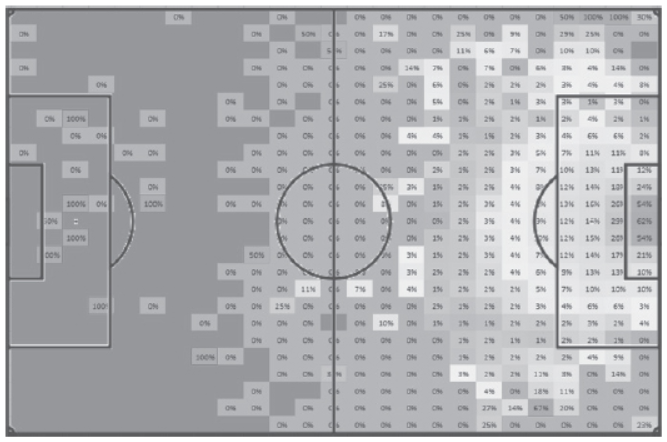
\includegraphics[scale=.75]{images/shot analysis.PNG}
    \caption{Shot Analysis}
    \label{fig:shot analysis}
    \cite{biermann2019football}
\end{figure}

In his work, the author \citeauthor{biermann2019football} has offered a thorough explanation of how football strategies are developed using the xG measure. Football is a game of probability, as was stated in the previous section \ref{football}. The likelihood that a wonder goal will be scored from various locations on the football field is shown in the figure \ref{fig:shot analysis}. The application of xG metric is demonstrated in this investigation. The shot's viewpoint was also taken into account in order to give this statistic additional context. For instance, shots from a distance of 12 yards have a higher likelihood of being successful than headers do, as do shots from counterattacks since the opposing defence is more unfocused in these circumstances. There are specific probability for attempts made in dead-ball situations as well. 

Additionally, as seen in figure \ref{fig:expectedgoals}, the work \cite{biermann2019football} has also emphasised time series graphs that indicate how goals scored correspond to goal scoring possibilities. 

\begin{figure}[!h]
    \centering
    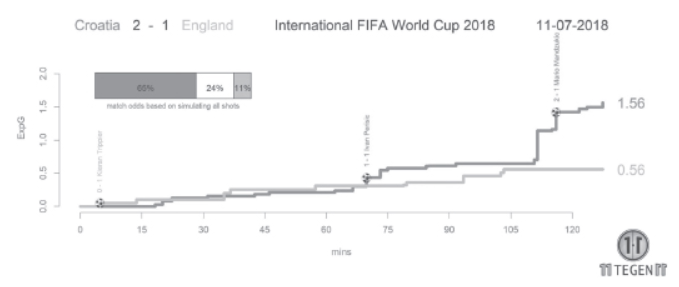
\includegraphics[scale=0.75]{images/expected goals.png}
    \caption{Time Series Graph}
    \label{fig:expectedgoals}
    \cite{biermann2019football}
\end{figure}

These methods have aided managers and coaches in putting tactics into practise that have improved player placement and game play. 

\citeauthor{rathke2017examination} looked at goals scored in European football leagues to determine whether factors are related to predicting expected goals (xG). This idea helped them evaluate players, especially strikers, according to the number of goals they score year after year. As a consequence, this research examined shots from 380 and 306 Premier League and Bundesliga games played in the 2012–2013 seasons, respectively. On the playing field, all of the shots were separated into regions, and each region was given a hypothetical goal value. The shot's distance from the goal and angle with respect to the goal were two factors that were looked at. It was postulated that the shots' range and aiming angle had an impact on the calculation of xG. \cite{rathke2017examination} The middle-of-the-table teams' goals and goals against were precisely identified by the algorithm. Teams at the top and bottom performed poorly, correspondingly. 

The model created in \cite{rathke2017examination} only took into account two aspects, but it may still be improved. Additionally, it hasn't been tested with newer data. 

\begin{figure}[!h]
    \centering
    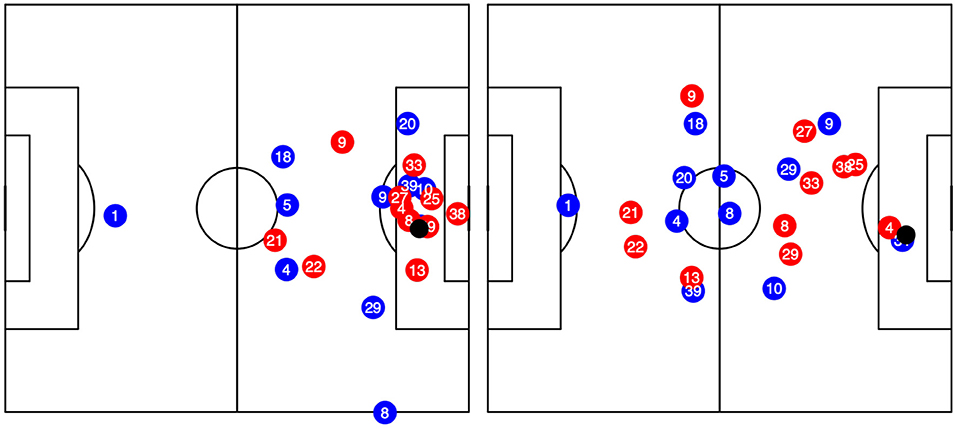
\includegraphics[scale=0.35]{images/anzer.jpg}
    \caption{Gabriel Anzer and Pascal Bauer}
    \label{Gabriel Anzer}
    \cite{anzer2021goal}
\end{figure}

The authors \citeauthor{anzer2021goal} assessed the calibre of each individual shot in their own model that investigates the xG metric. \cite{anzer2021goal} Their strategy has been examined by seasoned football experts and scientifically proven. The best model uses the XGBoost methodology and was constructed using precisely calibrated parameters obtained from synchronizing positional and event data of 105,627 shots in the Football League played in Germany. More precision than any other model that has been formally published may be shown in this model. This model has a 0.197 RPS (ranked probability score). 

Another study \cite{madrero2020creating} considered the ability of the shooter from different data-sets. The features that this considered were, Long Shots, Finishing, Heading, Shooting and Weak Foot. Along with these features there were other features that includes, x and position of the player, player ability, post rebound, back pass etc. An ANN (Artificial Neural Network) was implemented along with XGBoost algorithm and Logistic Regression with XGBoost performing the best. Due to lack of data the models were rather poor in performance. The best performing model for this study was XGBoost Algorithm.

\begin{figure}[!h]
    \centering
    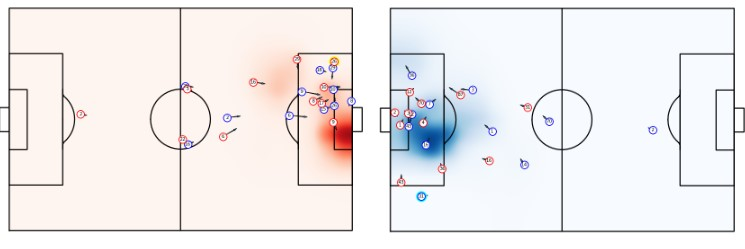
\includegraphics[scale=0.75]{images/spear.jpg}
    \caption{Time Series Graph}
    \label{Off Ball Scoring}
    \cite{spearman2018beyond}
\end{figure}


Many methods have been developed to assess the quality of soccer shots. In this work, we assess the efficiency of off-ball positioning prior to shoots that potentially result in goals. Consider a tall, unmarked centre forward who is positioned near the far post during a corner kick. When the cross comes in, the centre forward simply heads it in; other times, the cross sails over his head. Another example is a winger playing onside while breaking through the defensive line. Sometimes the through-ball arrives; other times, the winger may cut their run short when a teammate fails to provide a timely pass. Even though they never got the ball, the offensive player has generated a chance in both cases. The author \citeauthor{spearman2018beyond} \cite{spearman2018beyond} built a probability and physics-based model that leverages spatiotemporal player monitoring data to assess such off-ball scoring possibilities in this research (OBSO). This model may be used to predict which players, if any, are most expected to score at any moment throughout the game, as well as where on the field they are likely to score. The author demonstrates three significant applications of their model:
\begin{enumerate}
    \item Identifying and analysing key opportunities throughout a game
    \item to aid opposition analysis by indicating areas of the pitch where individual players or clubs are more likely to produce off-ball scoring chances.
    \item to automate talent discovery by identifying players throughout a whole league who excel at providing off-ball scoring opportunities. 
\end{enumerate}

\section{Summary}
The studies analysed in this section consolidated the nature of this case study and confirmed that the direction undertaken is a fruitful path with a lot of potential answers to how data science can be used in football. Furthermore, the works analysed in this study also highlight the future work of the metric that was developed in this study.
\chapter{Methodology}\label{meth}

\section{Data Specification}

All data in this study comes from StatsBomb's open data \cite{Statsbomb}, which is published free of charge as JSON files. Three kinds of file were used:
\begin{itemize}
    \item Competition Data: the competitions and seasons that are available
    \item Match Data: the matches of each competition and season, with teams and scores
    \item Event Data: every on-ball event of each match (passes, dribbles, tackles, shots and so on), and for each shot a \textit{freeze frame} giving the position of every visible player at the moment of the shot
\end{itemize}

\begin{figure}[!h]
    \centering
    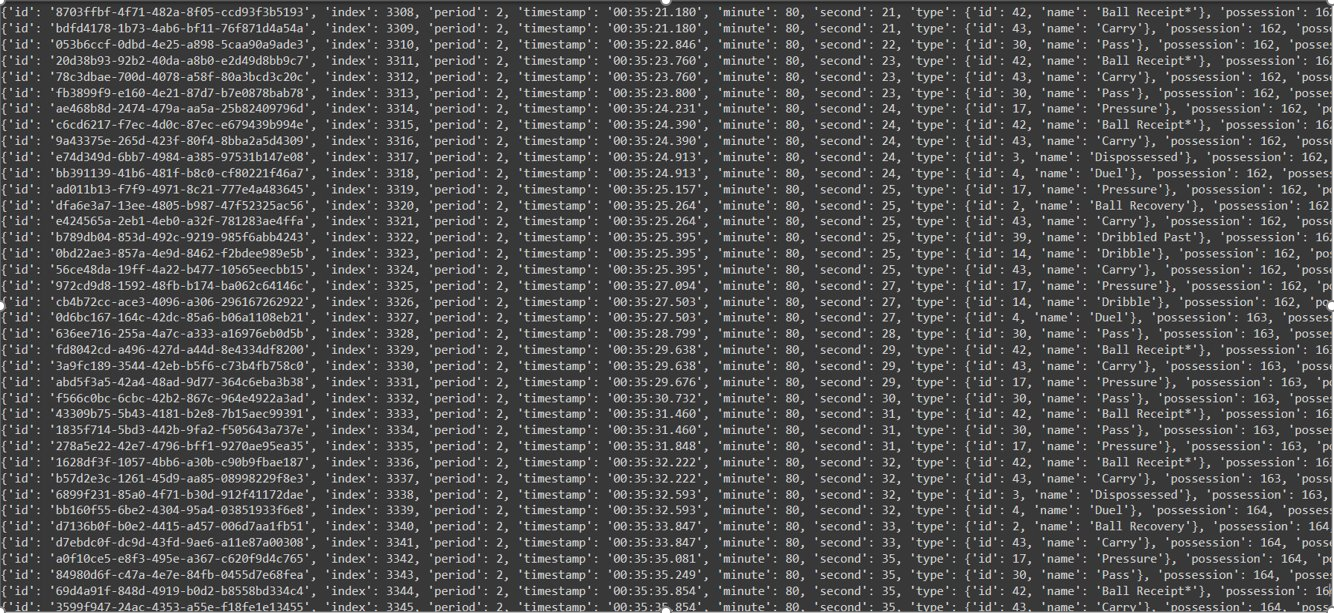
\includegraphics[scale=0.45]{images/data.png}
    \caption{Event Data Format}
    \label{data}
\end{figure}

A visual of the event data is shown in figure \ref{data}, where each row is one event of a 90 minute football match.

\subsection{Scope of the Revised Edition}

The original edition of this study used the 520 La Liga matches available in the open data at the time, all of which involved FC Barcelona. A model trained on one exceptional team learns that team's chances rather than football's, so this edition uses every men's match in the open data instead. Women's football is left out, so that the model describes one population of players.

The men's open data contains 2,651 matches and 66,854 shots, from La Liga, the Premier League, Serie A, Ligue 1, the 1. Bundesliga, the Indian Super League, the FIFA World Cup, the UEFA Euro, the Copa América, the African Cup of Nations, the Champions League and a few smaller competitions. Four of these are complete seasons: the 2015/16 Premier League, La Liga, Serie A and Ligue 1 (Ligue 1 is missing 3 of its 380 matches). The other competitions cover selected matches, such as one club's matches or a tournament.

The \textbf{modelling set} is every open-play shot from men's matches played since 2000, taken with the foot or the head: \textbf{61,003 shots and 6,277 goals (10.3\%) from 2,616 matches}. The 35 matches before 2000 were left out, because StatsBomb collected them from historical footage. Every open-play shot has a freeze frame, and 99.9\% of the freeze frames include the goalkeeper, so all the features below can be computed for the whole set.

The workflow used to develop the Expected Goals (xG) model has the following stages:
\begin{itemize}
    \item Data Cleaning/Wrangling
    \item Exploratory Data Analysis
    \item Feature Engineering
    \item Model Tuning and Evaluation
\end{itemize}

To visualise a football pitch, StatsBomb's coordinate system was followed. The pitch is 120 by 80 yards; the attacking goal is at $x = 120$, and its posts are at $y = 36$ and $y = 44$ (figure \ref{pitchspec}).

\begin{figure}[!h]
    \centering
    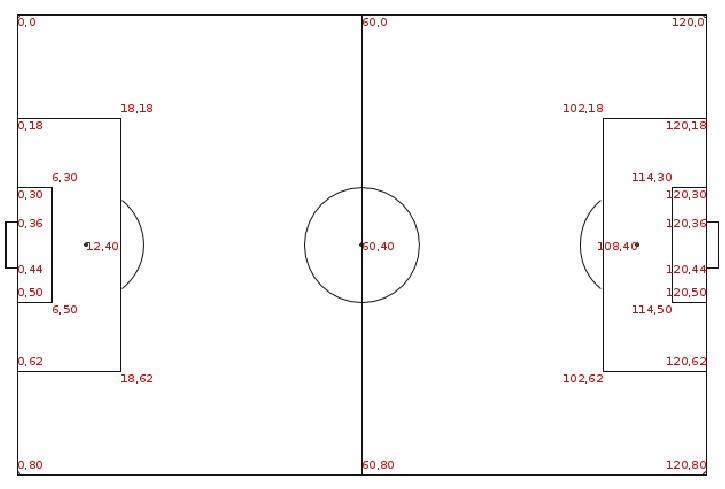
\includegraphics[scale=0.65]{images/pitchspec.jpg}
    \caption{Pitch Visualisation Specification}
    \label{pitchspec}
\end{figure}

\newpage

\section{Data Wrangling/Cleaning}

Data Wrangling is the process of turning raw data into a structured form that can be analysed. The events of every match were downloaded once and cached, and one row per shot was extracted with the following fields:

\begin{figure}[!h]
    \centering
    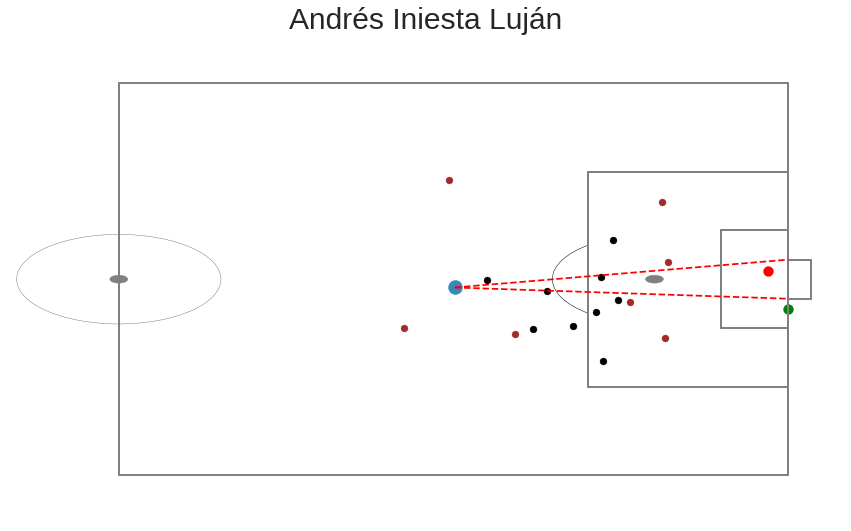
\includegraphics[scale=0.45]{images/angle.png}
    \caption{Football Pitch Visualisation}
    \label{example}
\end{figure}

\begin{itemize}
    \item Shot Id: ID of the Shot Event
    \item Play Pattern: Play Pattern preceding the Shot
    \item X Location Shot and Y Location Shot: Coordinates of the Shot
    \item Outcome: Outcome of the Shot
    \item Technique Used: The technique used to shoot the ball
    \item First Time: Whether the ball was shot with the first touch
    \item X GK Location and Y GK Location: Coordinates of the opposing Goalkeeper, from the freeze frame
    \item Body Part: The body part used
    \item Type of Shot: Open Play, Free Kick or Penalty
    \item Player Name and Team Name
    \item Official xG: xG provided by StatsBomb, kept only as a reference
    \item Pass Type: The height of the key pass before the shot (ground, low or high), or none
\end{itemize}

Two corrections were made compared with the original edition. First, the goalkeeper's position is now reset for every shot; previously, a shot whose freeze frame did not show the goalkeeper silently reused the position from the previous shot. Second, team names are taken from each match's line-ups, so that every shot is assigned to the right team. Further features were engineered from these fields, as covered in section \ref{feature}.

\newpage

\section{Exploratory Data Analysis}\label{EDA}

\begin{figure}[!h]
    \centering
    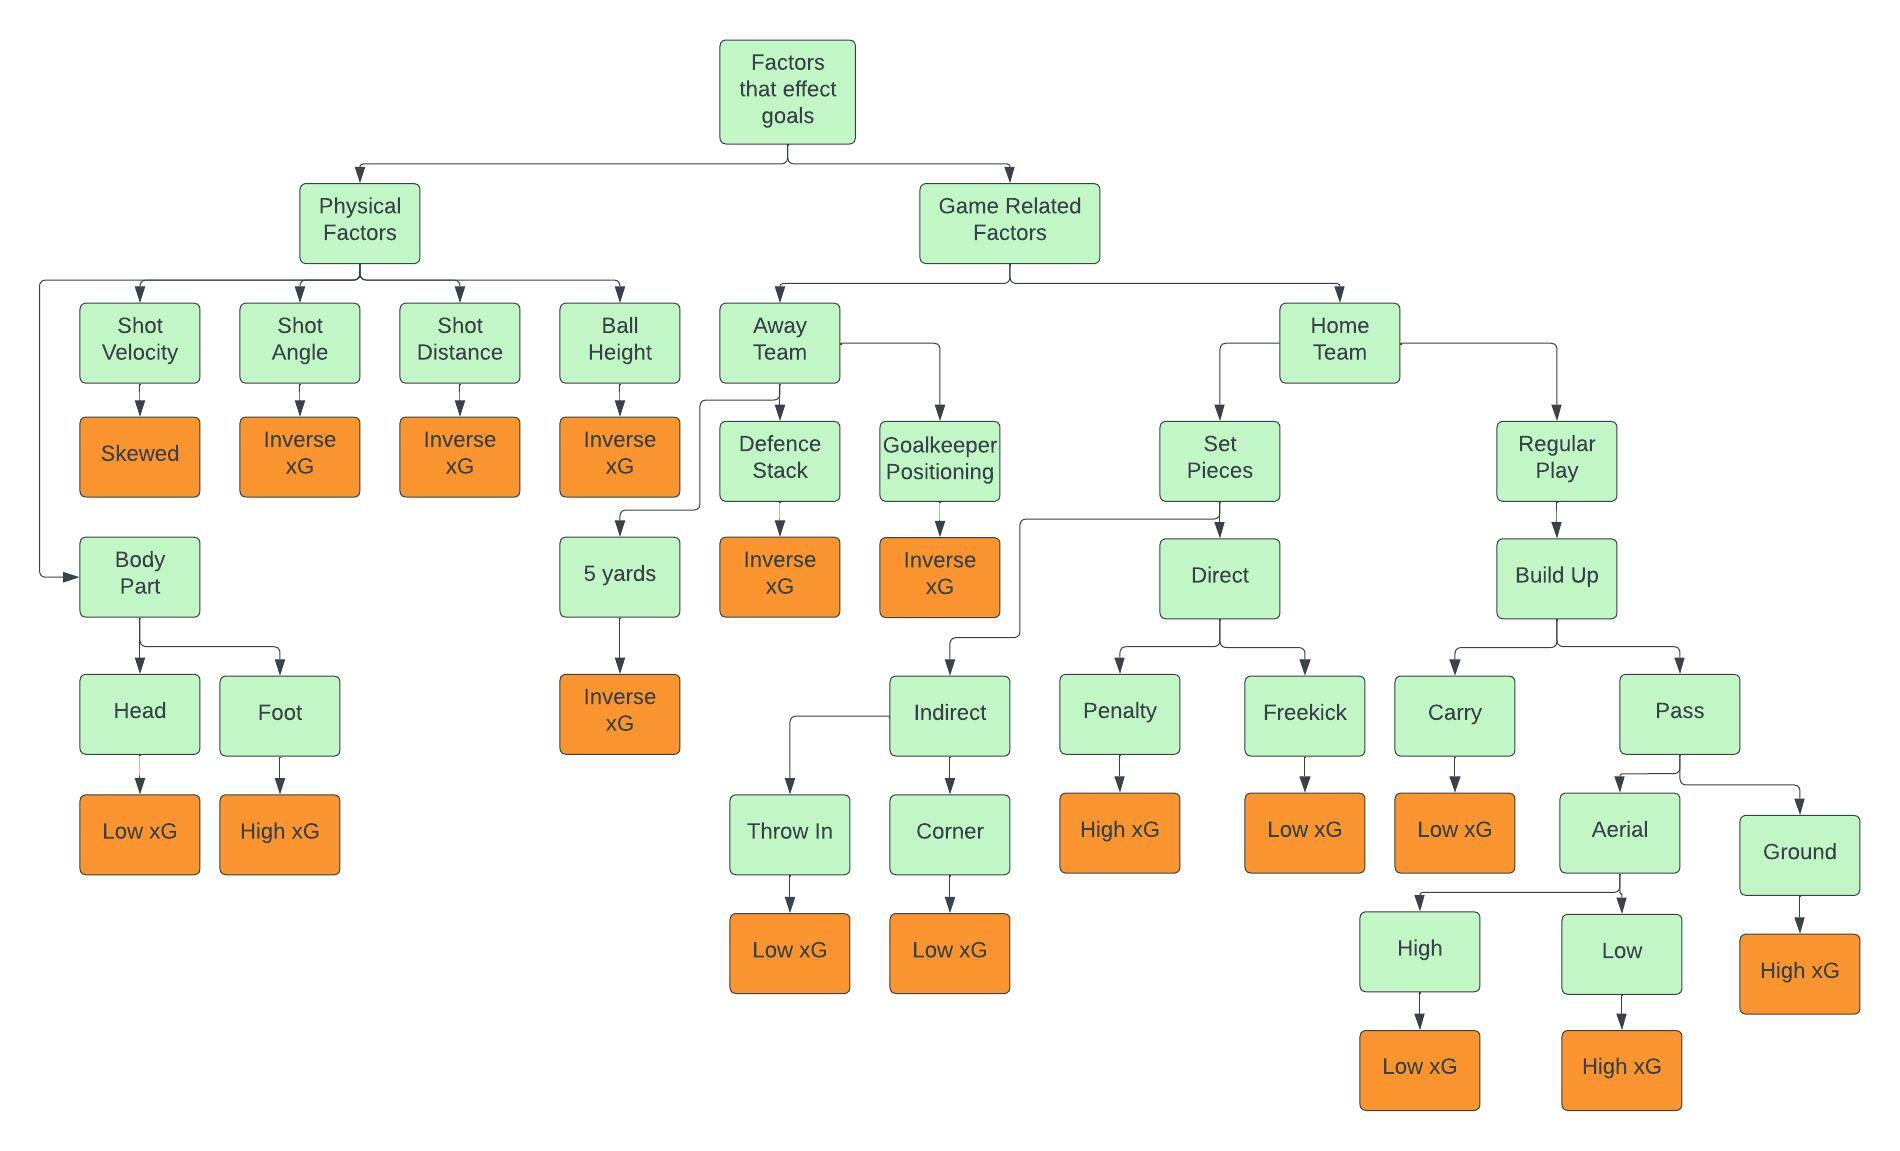
\includegraphics[scale=0.55]{images/hypothesis.jpeg}
    \caption{Hypothesis}
    \label{hypo}
\end{figure}

After the data was wrangled, it was explored to find which features matter for Machine Learning. An initial hypothesis directed this analysis and gave a road map for it (figure \ref{hypo}).

To keep the test of the models honest, the exploratory analysis uses only the \textbf{training matches}: 48,994 open-play shots and 5,024 goals (10.3\%) from 2,092 matches. The 524 matches held out for testing (section \ref{test}) were not looked at.

Many features in football are linked to shot distance: a shot close to goal is usually also taken under more pressure, at a wider angle, and more often with the head. A feature can therefore look important, or unimportant, only because of distance. Where this matters, the goal rate is compared \textbf{within bands of shot distance} as well as overall.

Each feature is analysed in turn, starting with Shot Distance.

\newpage

\subsection{Shot Distance}

Shot distance is the distance from the shot location to the centre of the goal. The hypothesis was that the chance of scoring falls with distance, and the data confirms it (figures \ref{shot distance} and \ref{histo}). More than half of all shots from within 5 yards were goals (56.4\%), against 22.3\% from 5--10 yards, 9.9\% from 15--20 yards and under 2.5\% from beyond 25 yards.

\begin{figure}[!h]
    \centering
    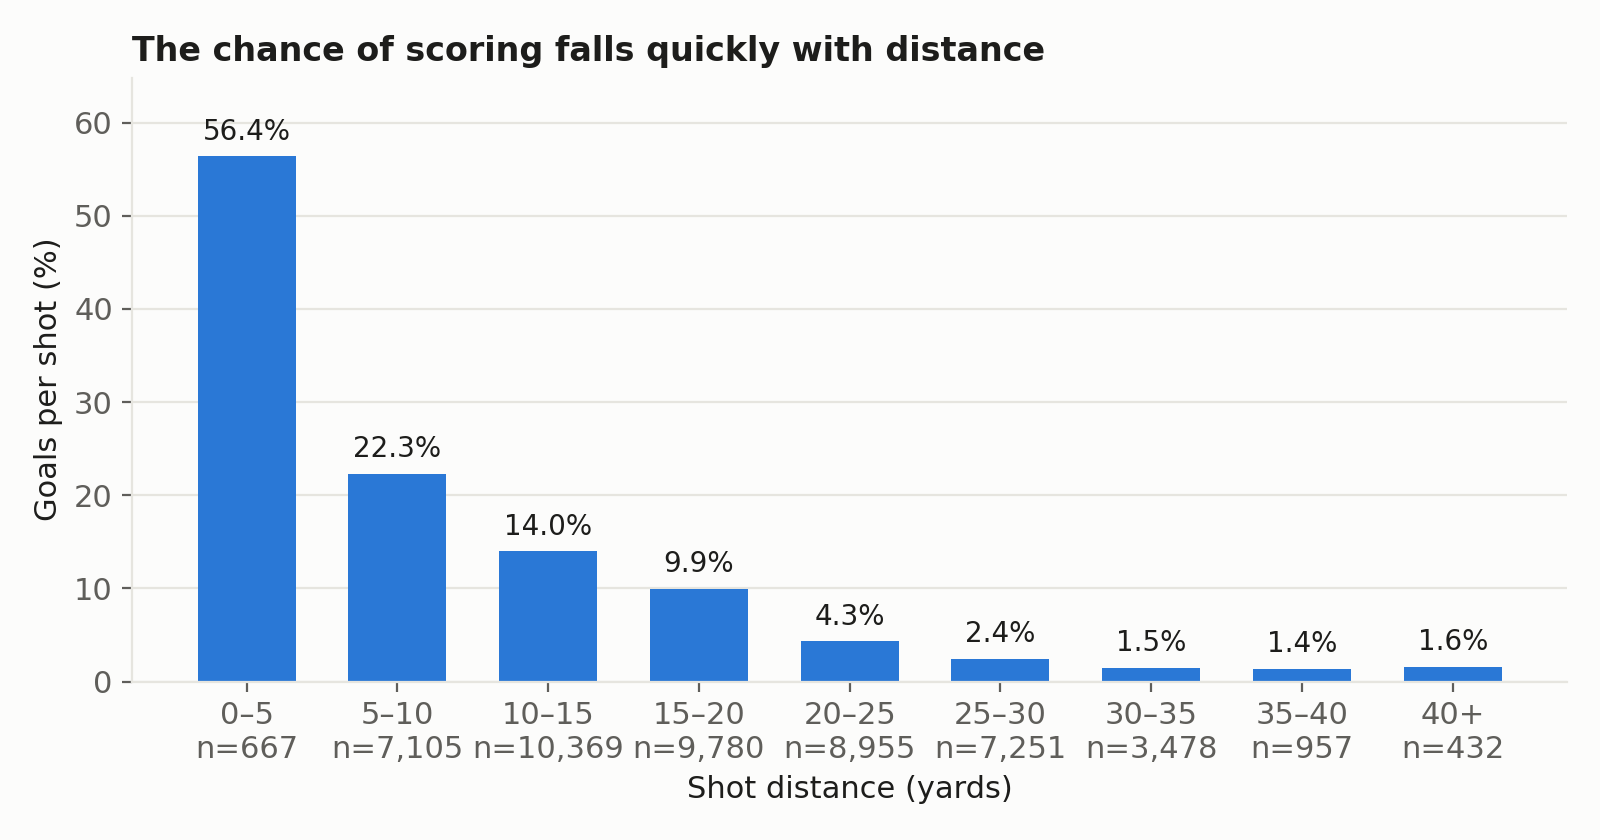
\includegraphics[width=0.9\textwidth]{images/shot distance.png}
    \caption{Goal Percentage in 5 yard Intervals}
    \label{shot distance}
\end{figure}

\begin{figure}[!h]
    \centering
    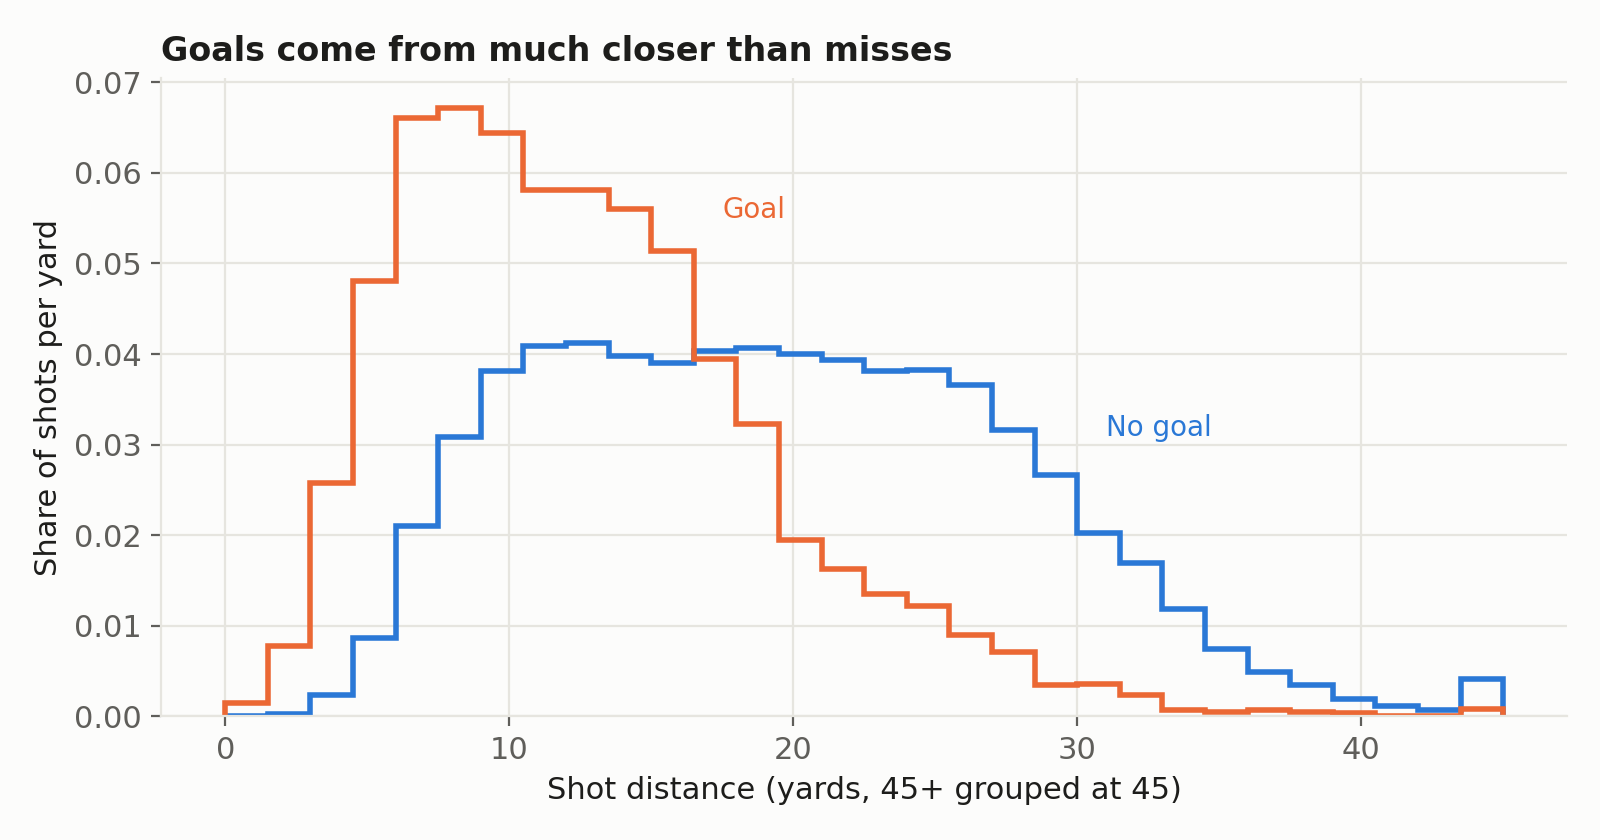
\includegraphics[width=0.9\textwidth]{images/histo.png}
    \caption{Shot Distance of Goals and Misses}
    \label{histo}
\end{figure}

88\% of goals were scored from inside the penalty area. Shot distance was therefore taken as a critical feature.

\newpage

\subsection{Shot Angle}\label{shotanglesec}

Consider the triangle formed by the shot location and the two goal posts. The Shot Angle is the angle of this triangle at the shot location, marked by the blue dot in figure \ref{shotangle}. The wider the angle, the more of the goal the shooter can see.

\begin{figure}[!h]
    \centering
    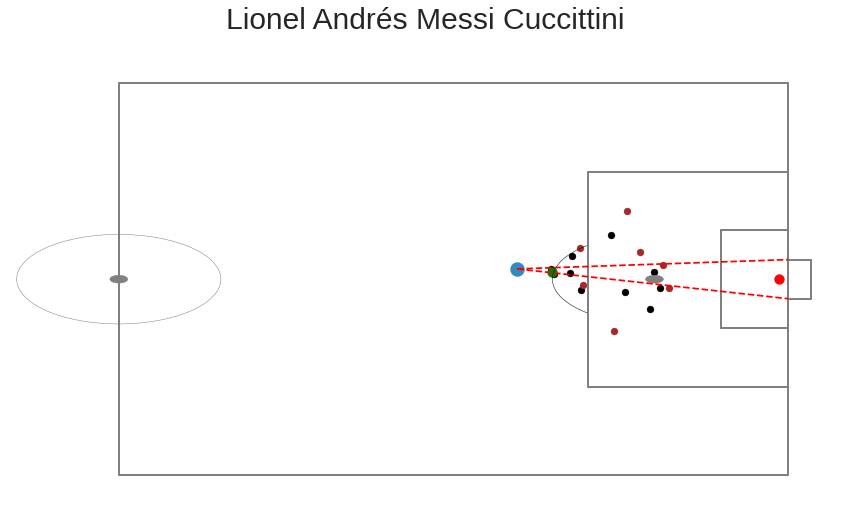
\includegraphics[scale=0.45]{images/messihalf.png}
    \caption{Shot Angle}
    \label{shotangle}
\end{figure}

Goals were scored from a median angle of 31.8°, against 19.1° for shots that did not result in a goal (figure \ref{shotangleplot}). The angle is closely related to distance, since shots from close in see more of the goal, but it also separates central shots from shots at the same distance from a tight angle.

\begin{figure}[!h]
    \centering
    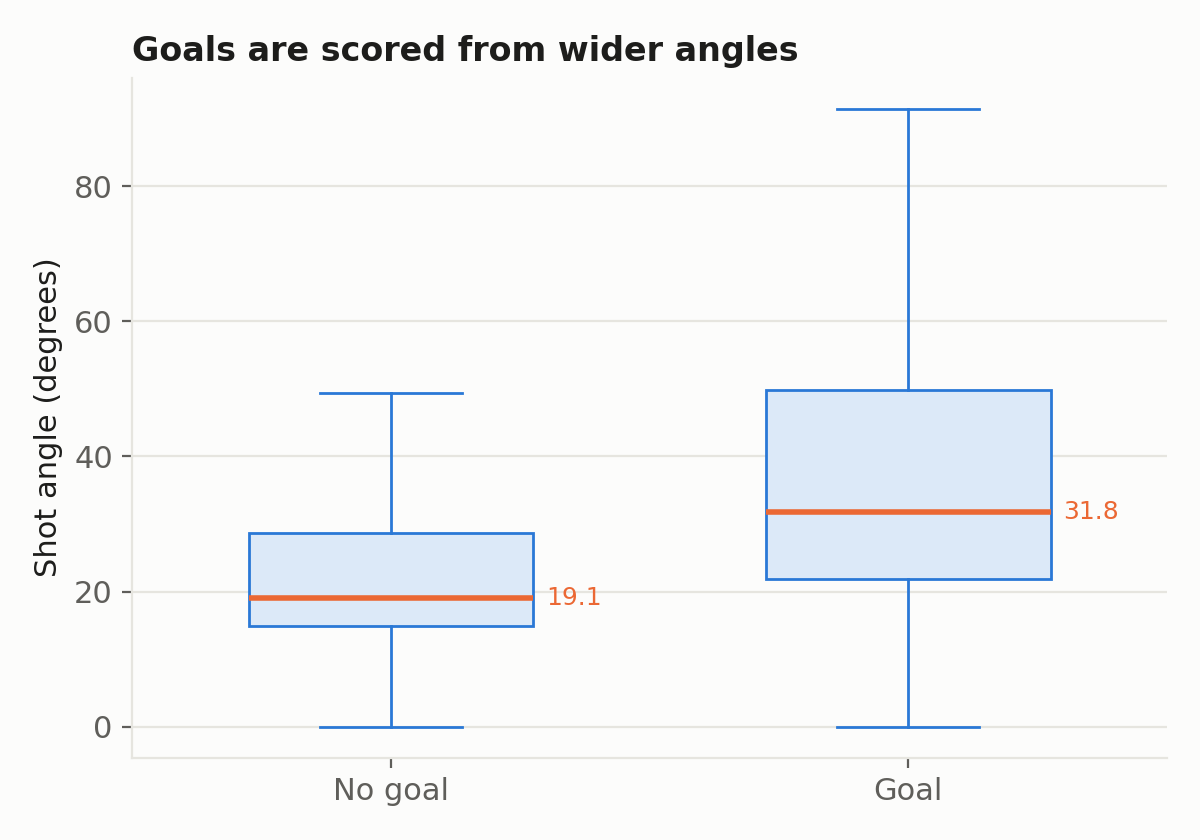
\includegraphics[width=0.6\textwidth]{images/angle1.png}
    \caption{Shot Angle of Goals and Misses (box plots without outliers)}
    \label{shotangleplot}
\end{figure}

\newpage

\subsection{Body Part}\label{bod}

There are two body parts that footballers use to shoot: the feet and the head. Any other body part is rare: only 154 of the 49,148 open-play shots in the training matches (0.3\%), and these were left out of the model (figure \ref{body}).

\begin{figure}[!h]
    \centering
    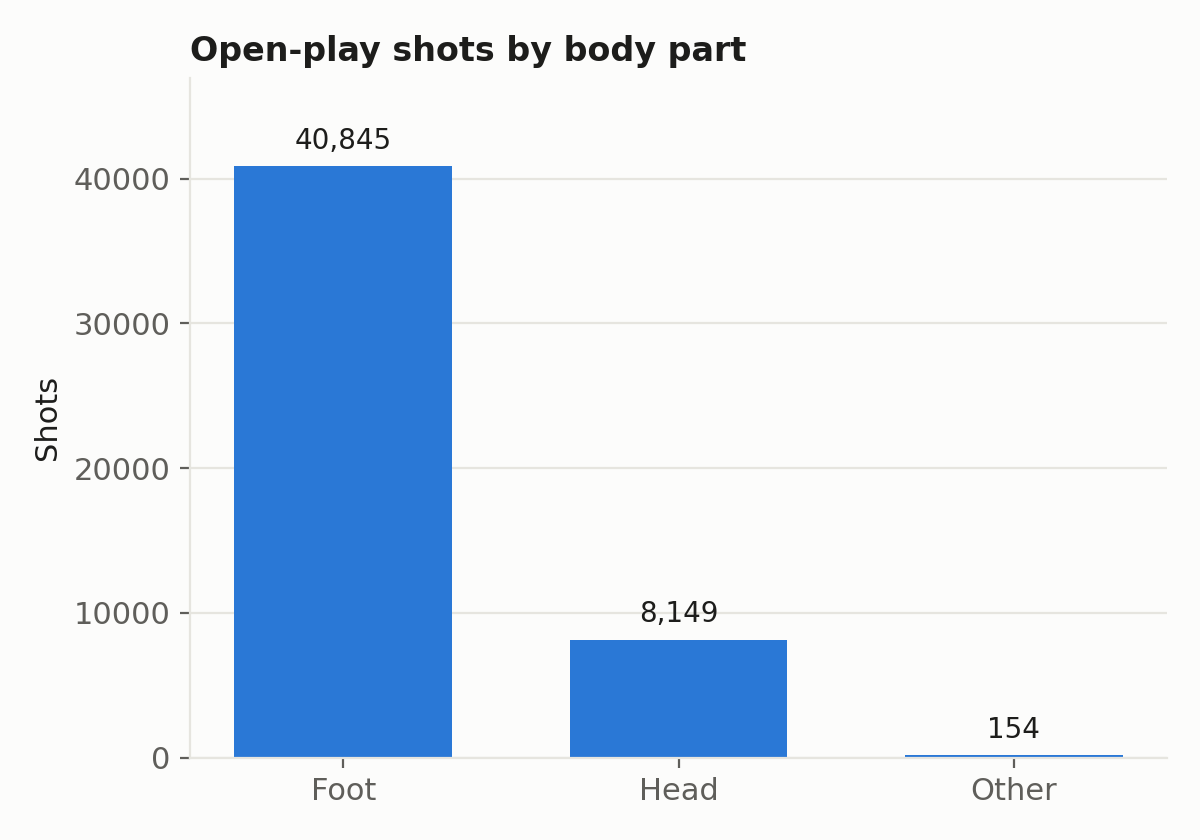
\includegraphics[width=0.6\textwidth]{images/body.png}
    \caption{Shots by Body Part}
    \label{body}
\end{figure}

Taken over all distances, shots with the foot and the head convert at almost the same rate: 10.2\% and 10.4\% (figure \ref{beforeskew}).

\begin{figure}[!h]
    \centering
    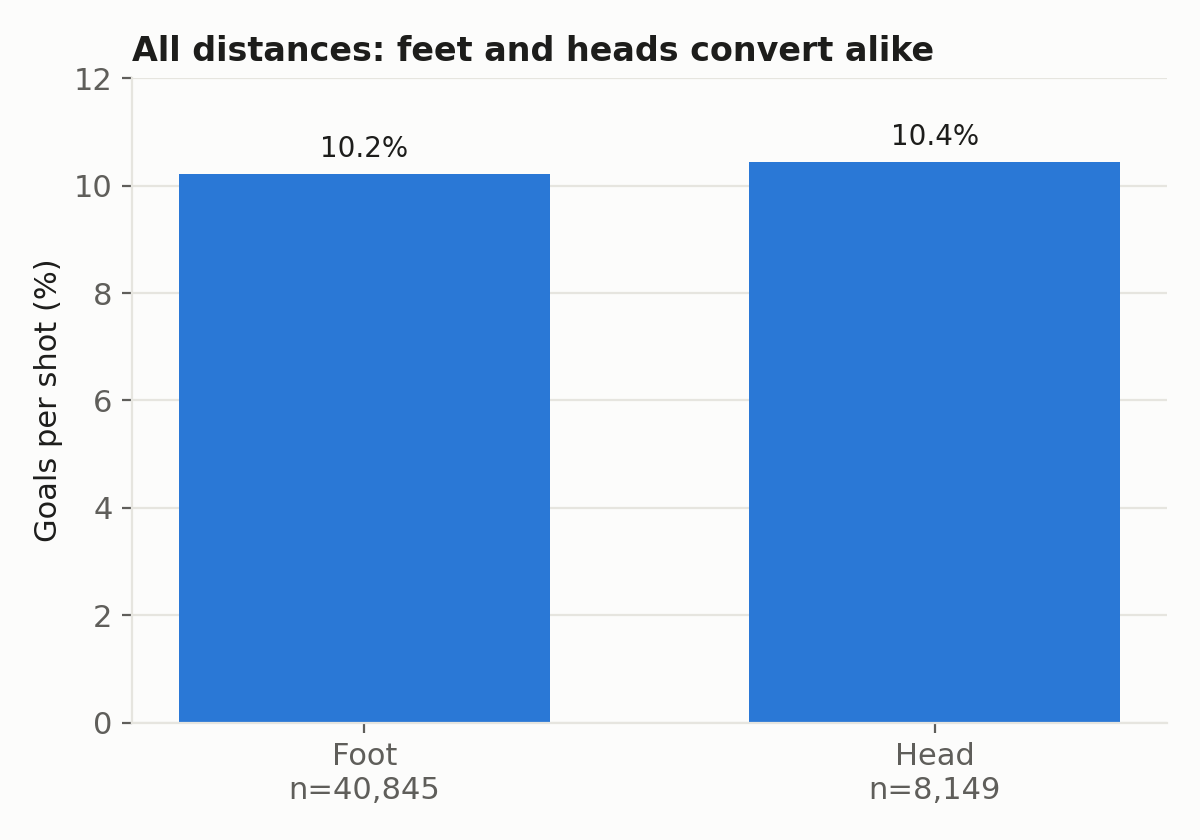
\includegraphics[width=0.6\textwidth]{images/beforeskew.png}
    \caption{Goals by Body Part, all Distances}
    \label{beforeskew}
\end{figure}

This comparison is misleading, because headers are taken much closer to goal. The median header is taken from 9.7 yards and the median shot with the foot from 20.3 yards, and 99\% of headers are taken from within 18 yards (figure \ref{bodybox}).

\begin{figure}[!h]
    \centering
    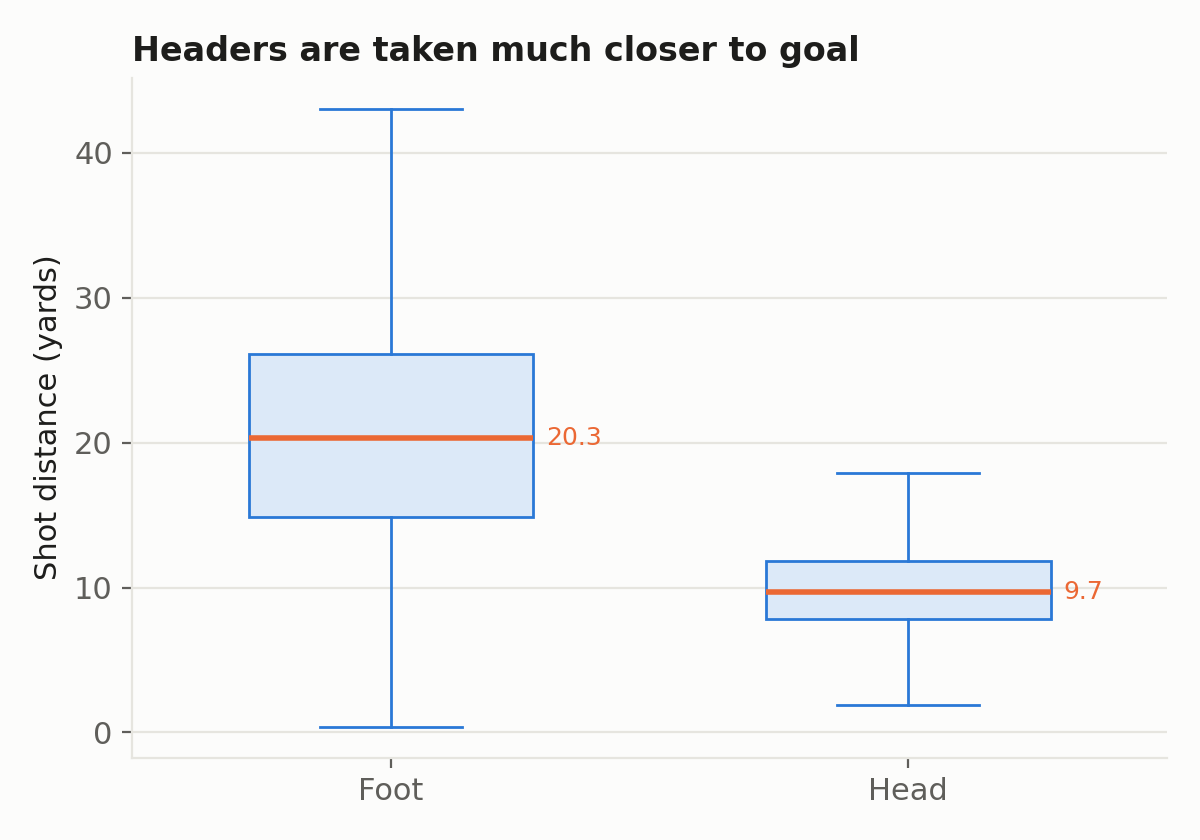
\includegraphics[width=0.6\textwidth]{images/bodybox.png}
    \caption{Shot Distance by Body Part (box plots without outliers)}
    \label{bodybox}
\end{figure}

When shots are compared at the same distance, the difference is large (figure \ref{afterskew}). Within 18 yards, 20.3\% of shots with the foot were goals, against 10.5\% of headers; under 12 yards the rates are 31.0\% and 12.5\%. As the hypothesis expected, a header is a much worse chance than a shot with the foot from the same place.

\begin{figure}[!h]
    \centering
    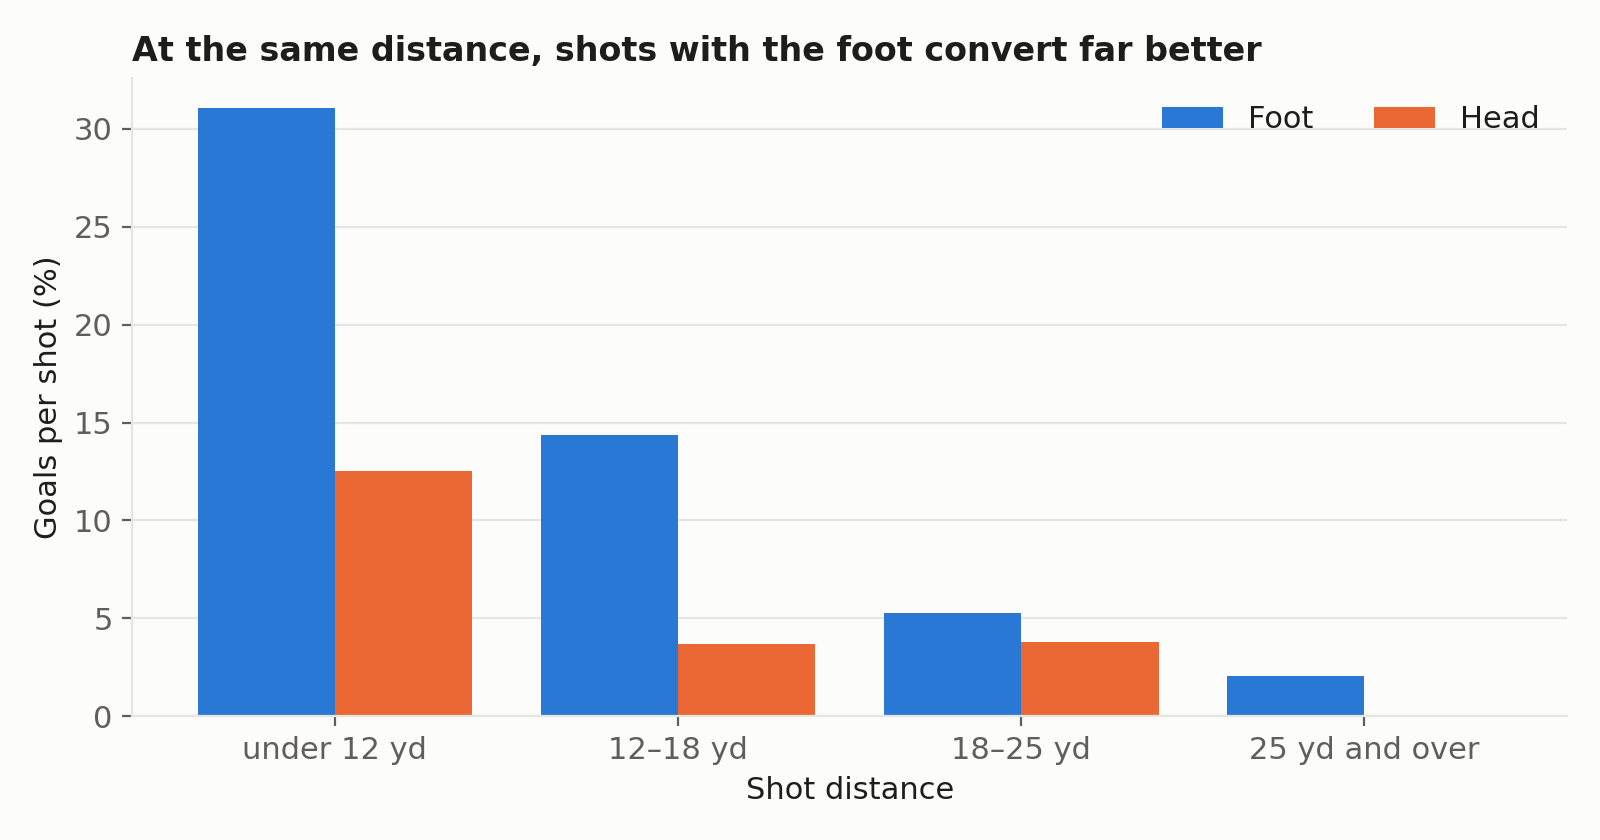
\includegraphics[width=0.9\textwidth]{images/afterskew.png}
    \caption{Goals by Body Part within Distance Bands}
    \label{afterskew}
\end{figure}

\newpage

\subsection{Pressure}\label{pressure}

When a player shoots, defenders close by can block the shot or hurry it. This was measured as the number of opponents within 5 yards of the shooter in the freeze frame.

Taken over all distances, pressure seems to make no difference: shots with 0, 1, 2 and 3 or more opponents within 5 yards convert at 9.9\%, 10.7\%, 10.0\% and 10.1\%. The reason is again distance. Pressure increases as the shot gets closer to goal: the median shot with no opponent nearby is taken from 24.8 yards, and with 3 or more from 12.8 yards (figure \ref{5yardsbox}).

\begin{figure}[!h]
    \centering
    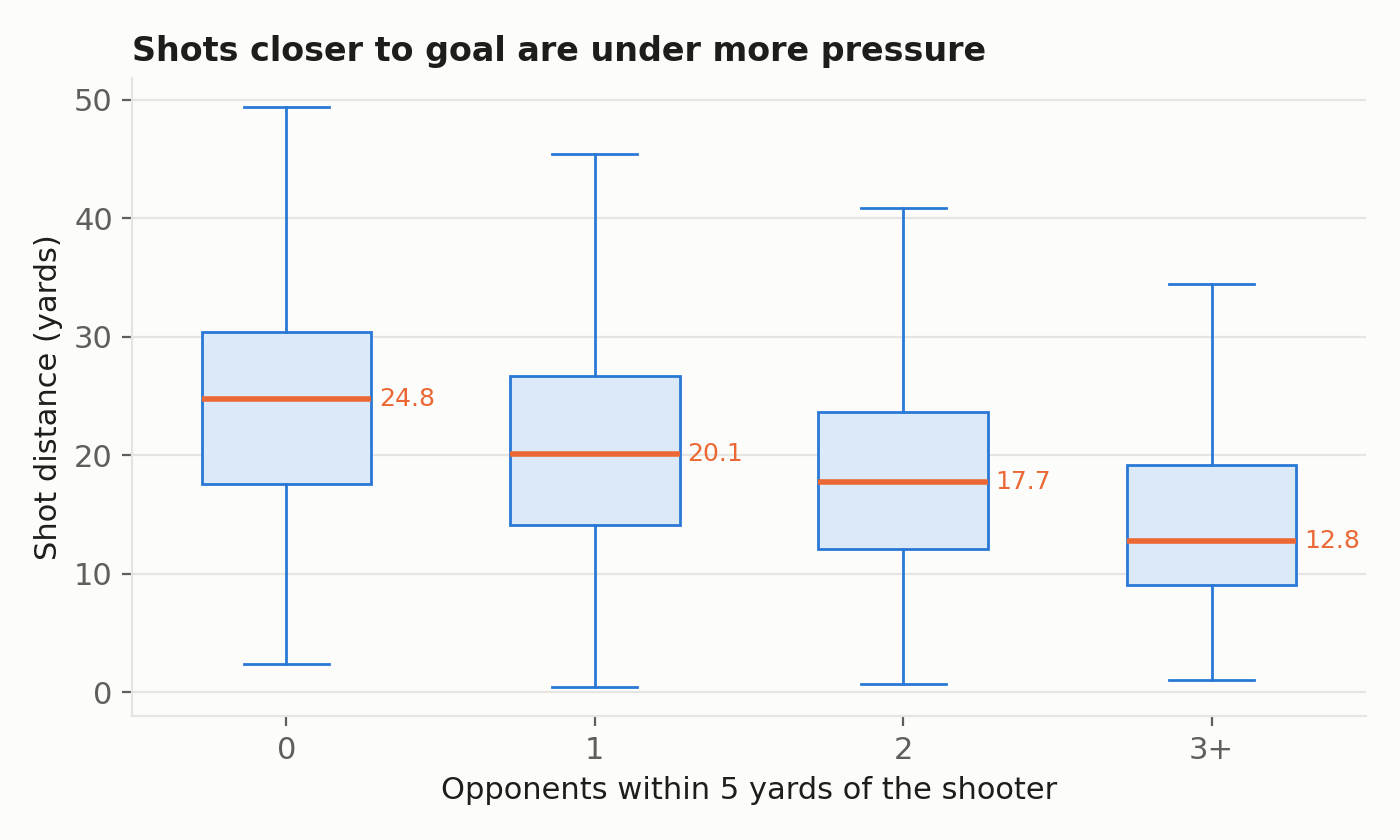
\includegraphics[width=0.75\textwidth]{images/5yardsbox.png}
    \caption{Shot Distance vs Pressure (box plots without outliers)}
    \label{5yardsbox}
\end{figure}

Within each distance band, the hypothesis holds (figure \ref{5yardsbar}). Under 12 yards, the goal rate falls from 40.9\% with no opponent nearby to 29.6\%, 21.4\% and 14.2\% with 1, 2 and 3 or more. The effect is smaller for long shots, which rarely go in whatever the pressure.

\begin{figure}[!h]
    \centering
    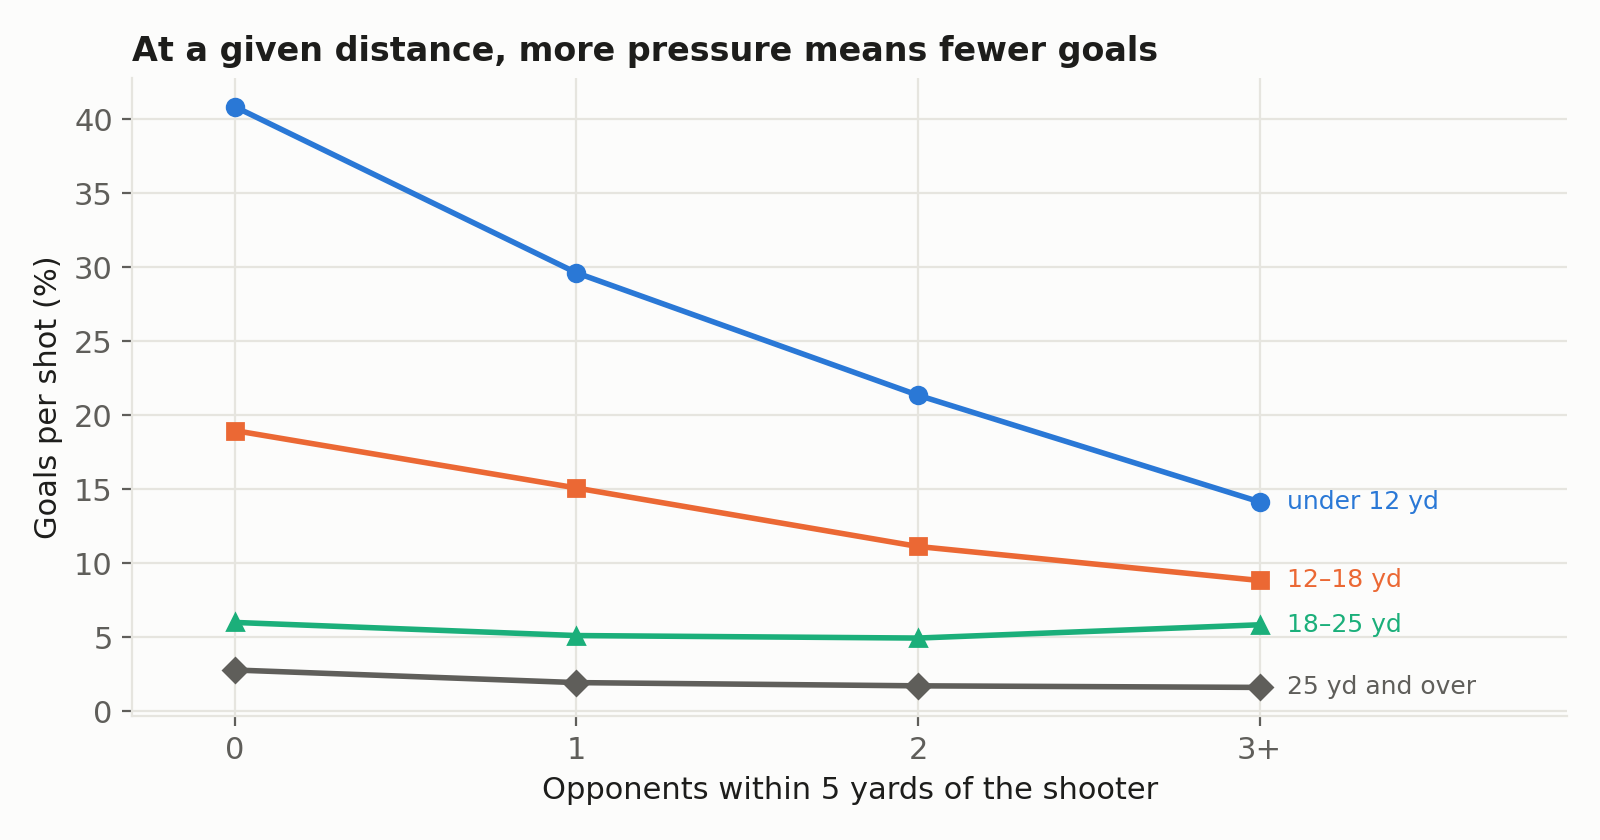
\includegraphics[width=0.9\textwidth]{images/5yardsbar.png}
    \caption{Goal Percentage vs Pressure within Distance Bands}
    \label{5yardsbar}
\end{figure}

\newpage

\subsection{Number of Players in front of Goal}

Consider again the triangle formed by the shot location and the two posts (figure \ref{shotangle}). Opponents inside this triangle, including the goalkeeper, stand between the ball and the goal and can block the shot (figure \ref{messi}). The number of opponents inside the triangle was counted from the freeze frame.

\begin{figure}[!h]
    \centering
    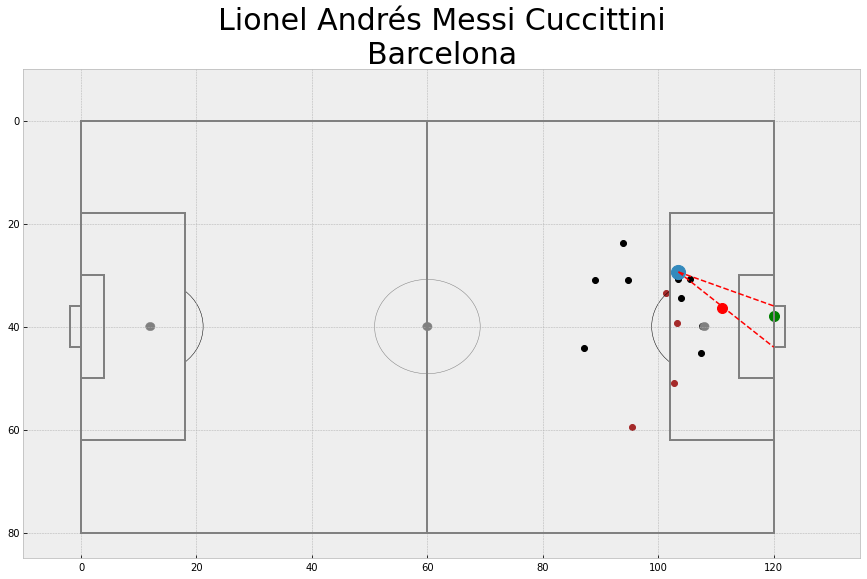
\includegraphics[scale=0.5]{images/messsiiii.png}
    \caption{Players between Goal}
    \label{messi}
\end{figure}

This feature has the strongest relation with goals of all the freeze-frame features (figure \ref{oppobtngoal}). With nobody in the triangle, which usually means the goalkeeper has been beaten or drawn out, 43.8\% of shots were goals. With one player in the way, usually only the goalkeeper, the rate was 13.0\%, and it fell to 5.8\%, 4.4\% and 3.5\% with 2, 3 and 4 or more.

\begin{figure}[!h]
    \centering
    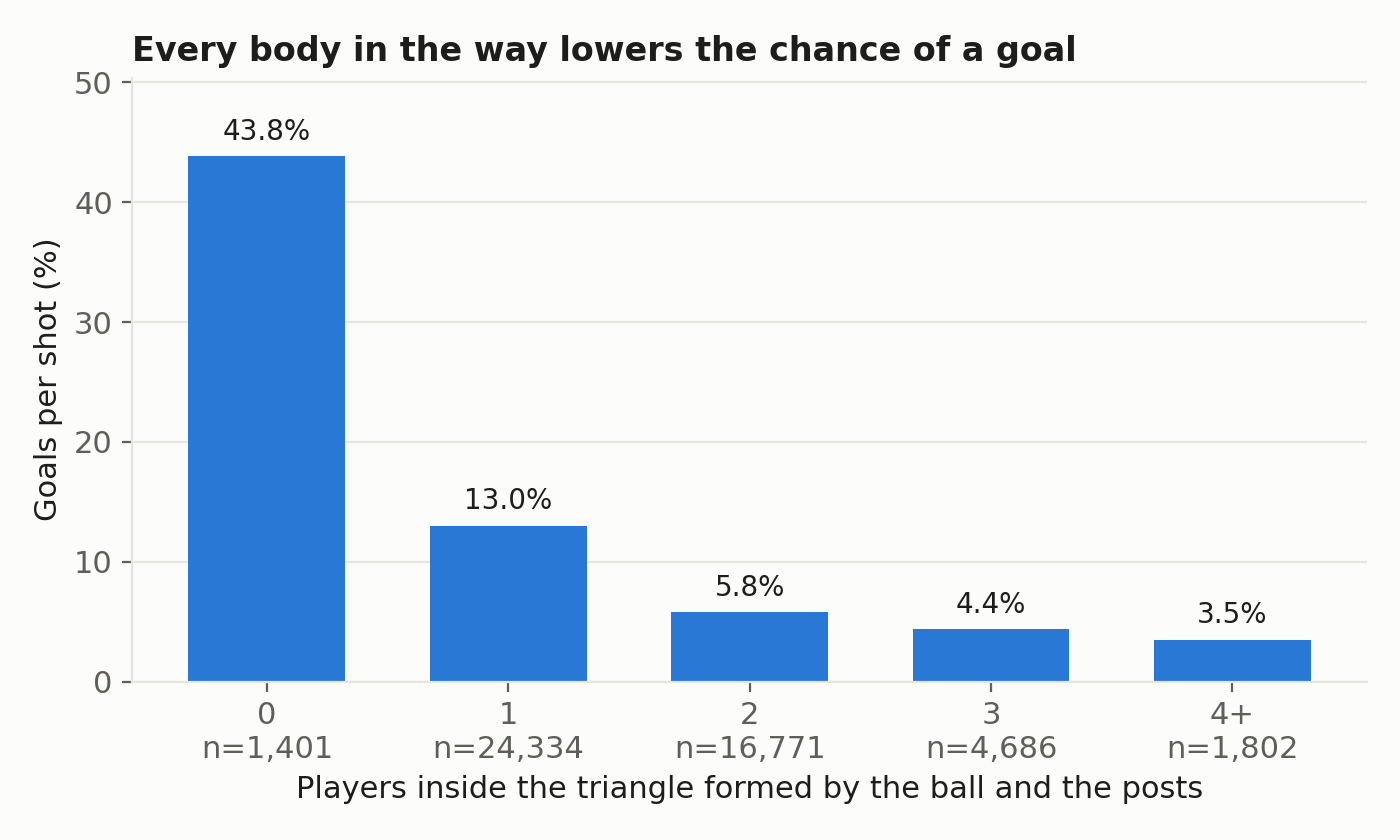
\includegraphics[width=0.75\textwidth]{images/opponentsbetweengoalbar.png}
    \caption{Goal Percentage vs Players between Ball and Goal}
    \label{oppobtngoal}
\end{figure}

The number of players in the way rises with distance, from a median distance of 9.9 yards with nobody in the triangle to about 21 yards with 3 or more (figure \ref{oppobtngoalbox}), since a longer shot passes through more of the pitch. Distance, angle and the players in the way therefore add up: a long shot from a tight angle through a crowded area has an xG close to zero.

\begin{figure}[!h]
    \centering
    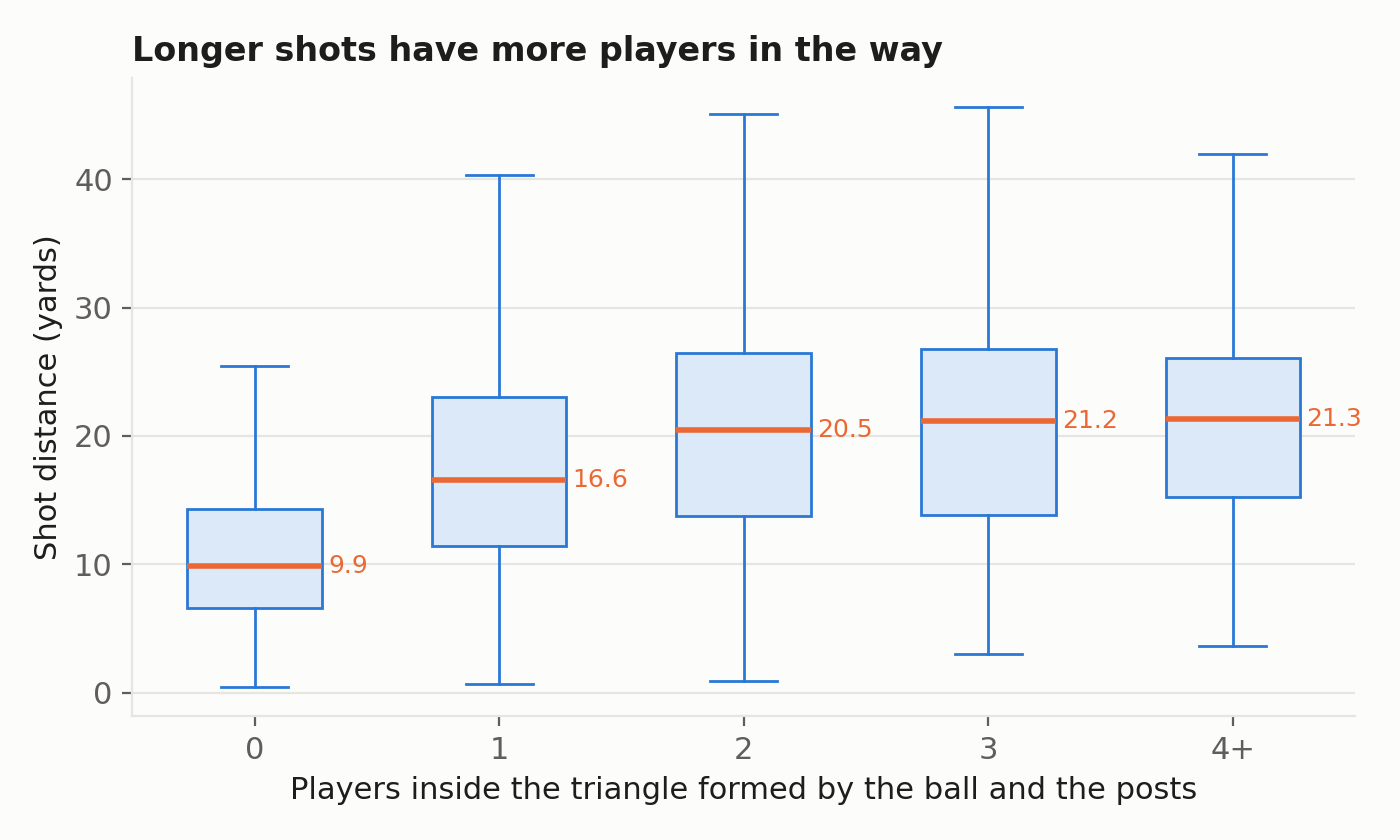
\includegraphics[width=0.75\textwidth]{images/opponentsgoalbox.png}
    \caption{Shot Distance vs Players between Ball and Goal (box plots without outliers)}
    \label{oppobtngoalbox}
\end{figure}

\newpage

\subsection{Goal Keeper Distance and Location}

Though a goalkeeper stays near the goal for most of a match, there are situations when he or she has to move away from it. In a one-on-one, for example, goalkeepers come towards the striker to narrow the angle. The goalkeeper's distance from the centre of the goal was therefore analysed.

\begin{figure}[!h]
    \centering
    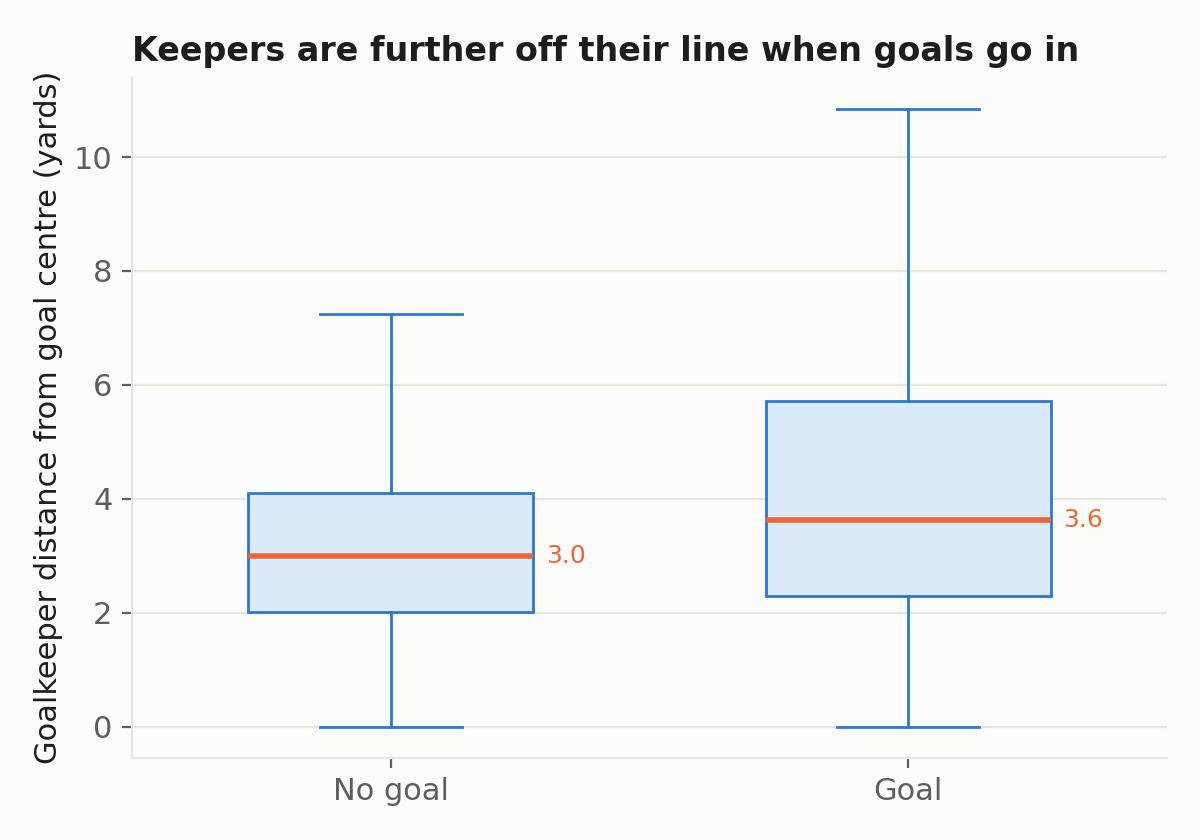
\includegraphics[width=0.6\textwidth]{images/gkdist.png}
    \caption{Goal Keeper Distance for Goals and Misses (box plots without outliers)}
    \label{gkdist}
\end{figure}

As the hypothesis proposed, goalkeepers were further from their goal when goals were scored: a median of 3.6 yards against 3.0 yards, and a mean of 4.6 yards against 3.4 yards (figure \ref{gkdist}).

\begin{figure}[!h]
    \centering
    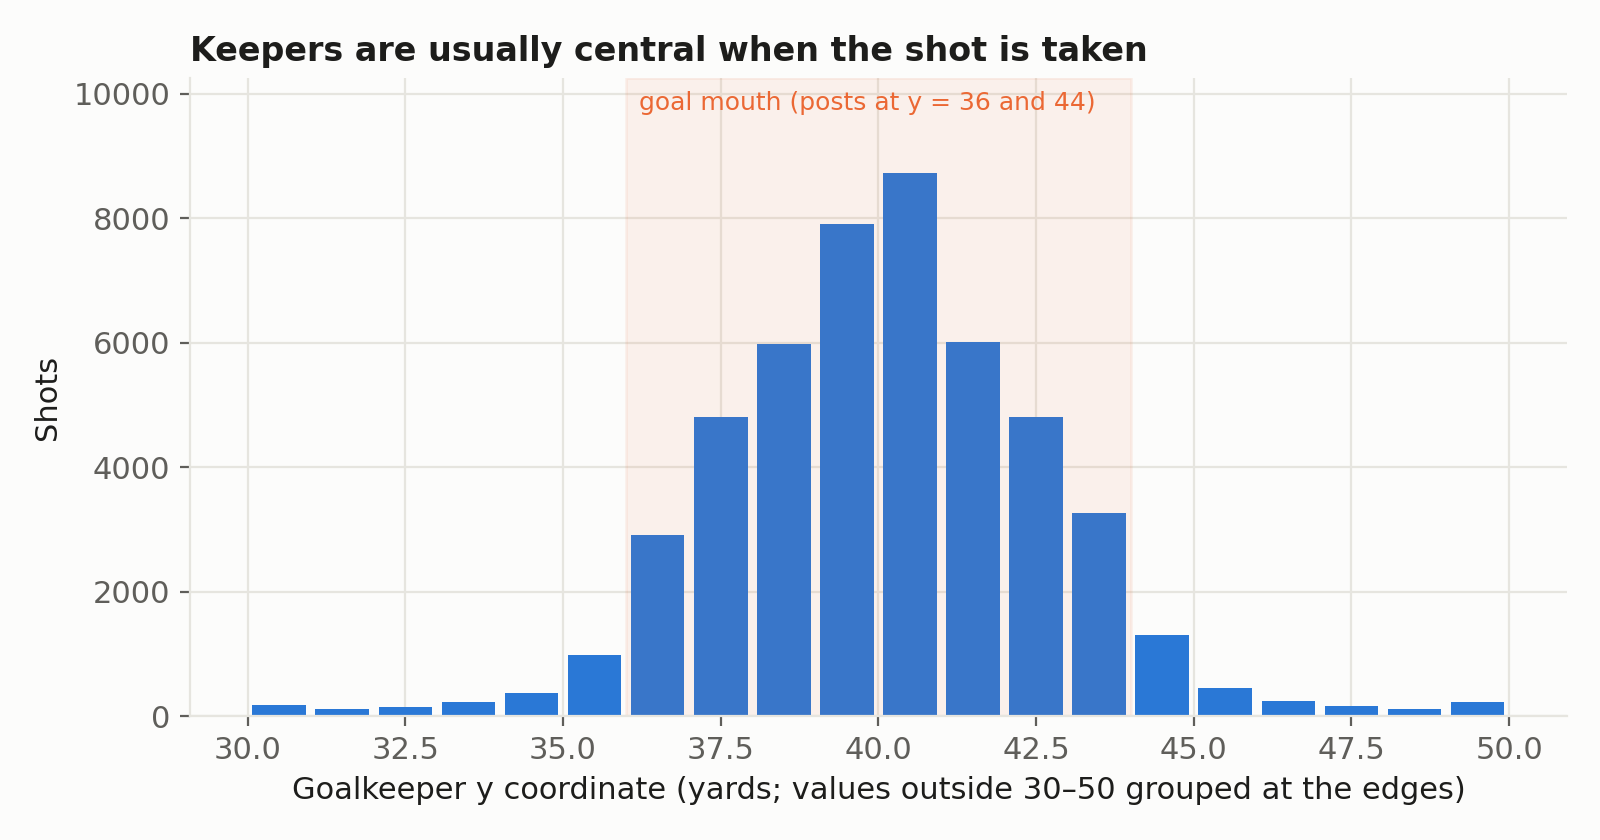
\includegraphics[width=0.9\textwidth]{images/ygkloc.png}
    \caption{Goal Keeper Y Coordinate at the Moment of the Shot}
    \label{ygkloc}
\end{figure}

The goalkeeper's y coordinate shows where they stand across the goal. Most shots were taken with the goalkeeper near the centre of the goal: in 60\% of shots the goalkeeper stood between $y = 38$ and $y = 42$ (figures \ref{ygkloc} and \ref{gkloc}). The goalkeeper's x and y coordinates were both included in the model.

\begin{figure}[!h]
    \centering
    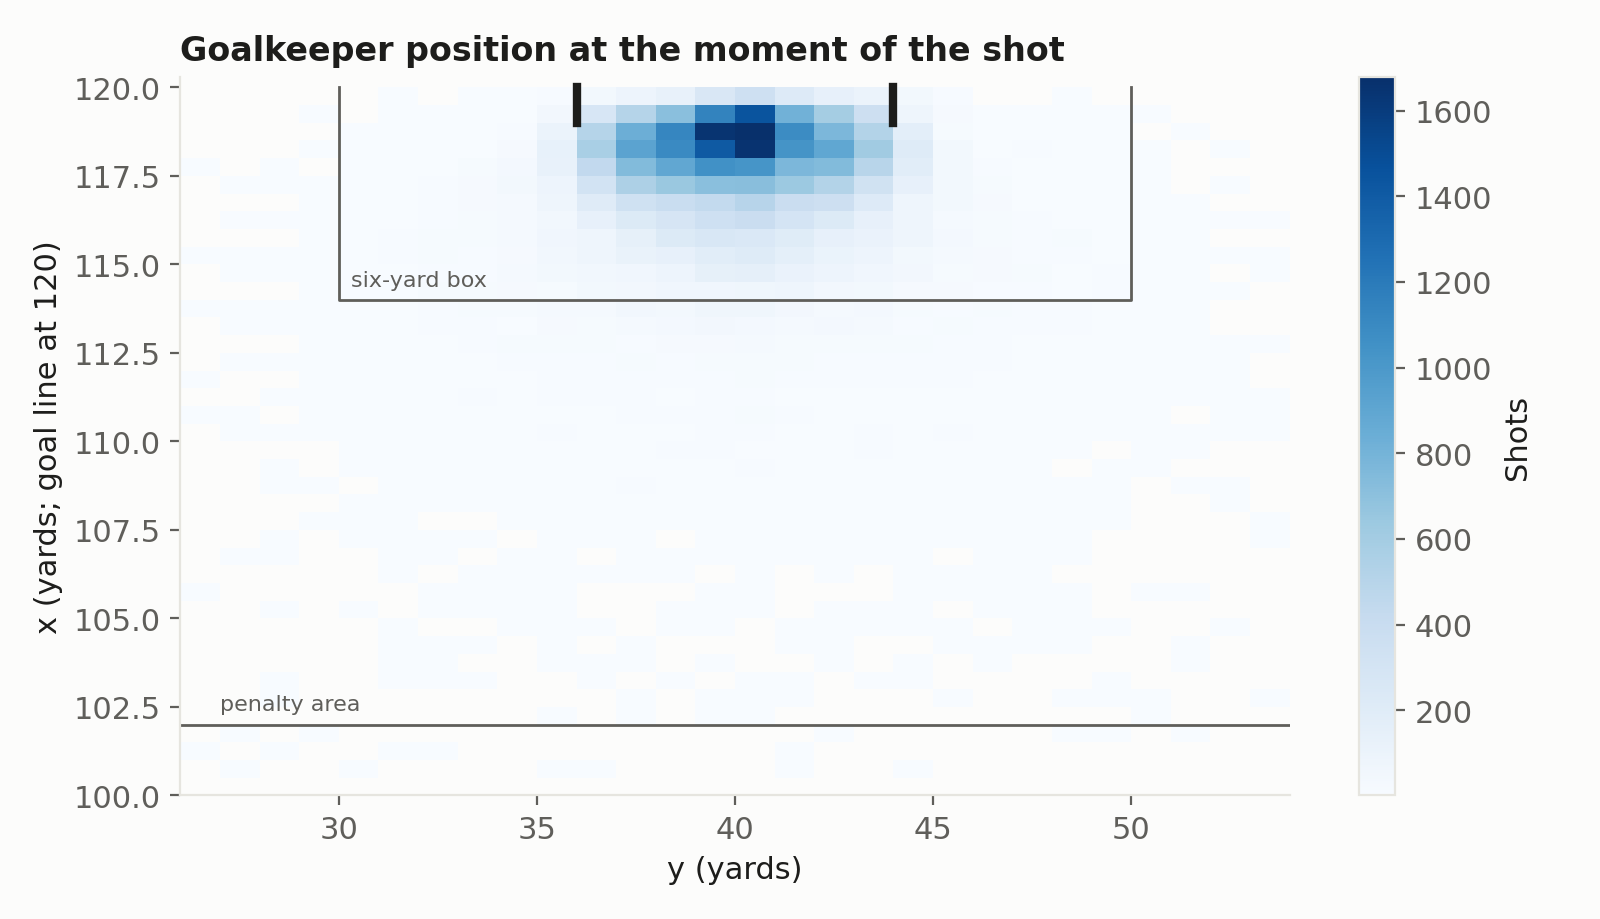
\includegraphics[width=0.9\textwidth]{images/gkloc.png}
    \caption{Goal Keeper Location at the Moment of the Shot}
    \label{gkloc}
\end{figure}

\newpage

\subsection{Preceding Play Pattern}

The play pattern describes the passage of play that led to the shot. The play patterns defined by StatsBomb \cite{Statsbomb} are:

\begin{itemize}
    \item 'From Counter': The event was part of a counter attack:
    \begin{itemize}
        \item The possession began with an open play turnover outside the counter-attacking team’s final third.
        \item The possession was at least 75\% direct towards goal.
        \item The attack travelled a minimum of 18 yards towards goal.
    \end{itemize}
    \item 'From Throw In': The passage of play after a throw-in.
    \item 'Regular Play': None of the other play patterns.
    \item 'From Corner': The passage of play after a corner.
    \item 'From Free Kick': The passage of play after a free-kick.
    \item 'From Goal Kick': The passage of play after a goal kick.
    \item 'From Kick Off': The passage of play after the kick off.
    \item 'From Keeper': The passage of play after a keeper distribution.
\end{itemize}

These play patterns describe the build-up to an open-play shot; they must not be confused with direct shots from set pieces, which are not part of this model. Most shots come from regular play, followed by throw-ins, free kicks and corners (figure \ref{playpatt}).

\begin{figure}[!h]
    \centering
    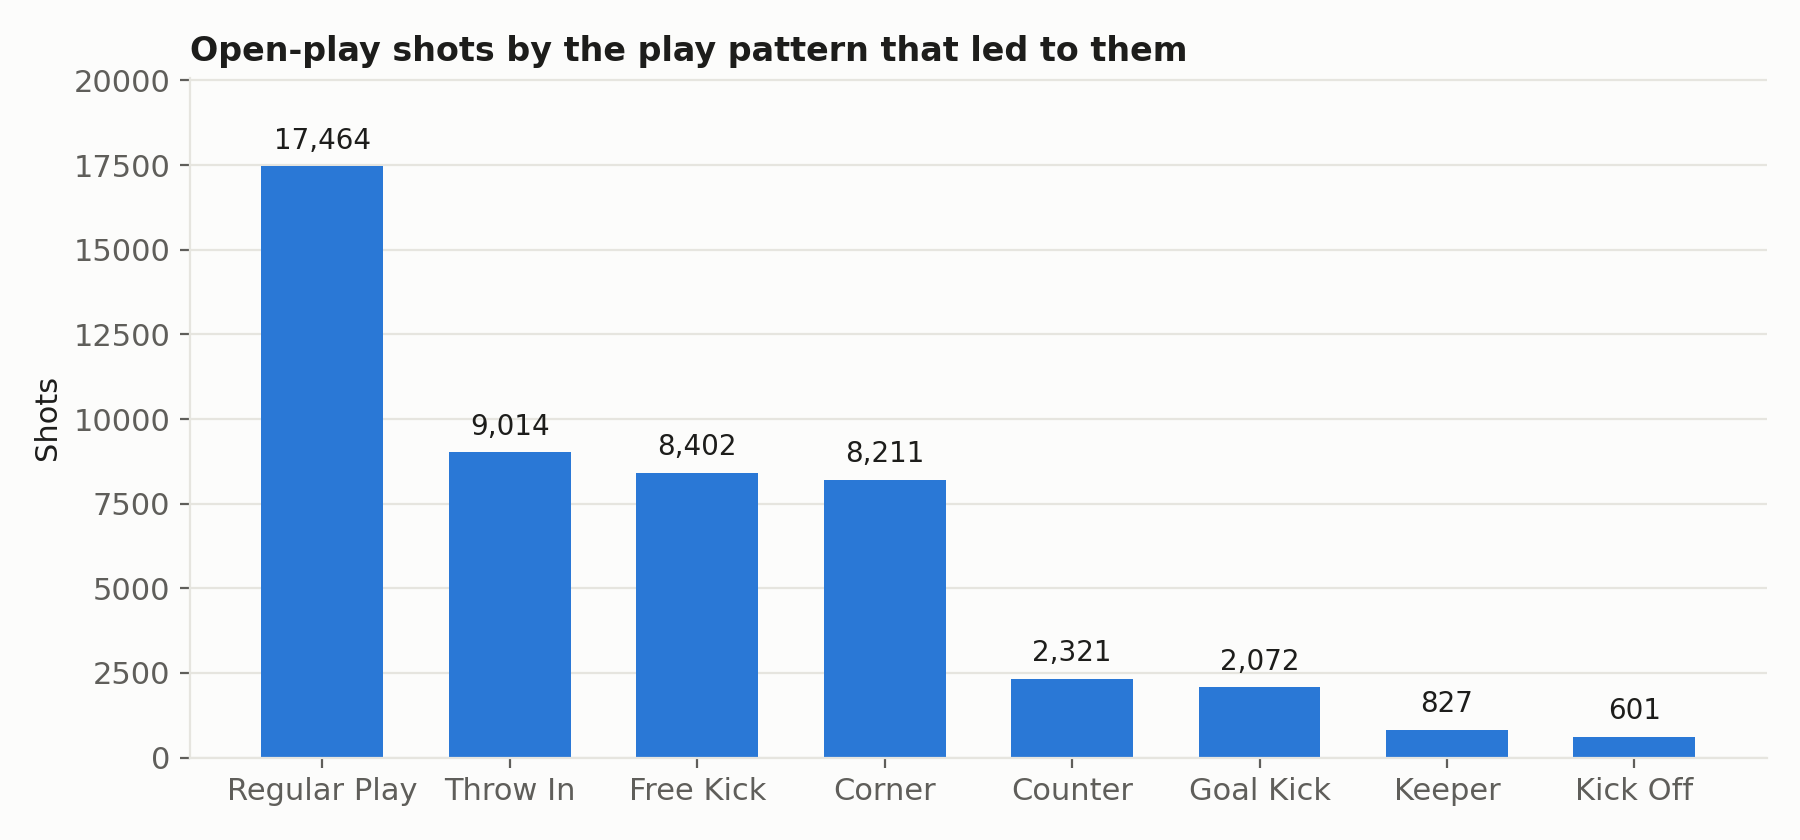
\includegraphics[width=0.9\textwidth]{images/playpatt.png}
    \caption{Shots by Play Pattern}
    \label{playpatt}
\end{figure}

\begin{figure}[!h]
    \centering
    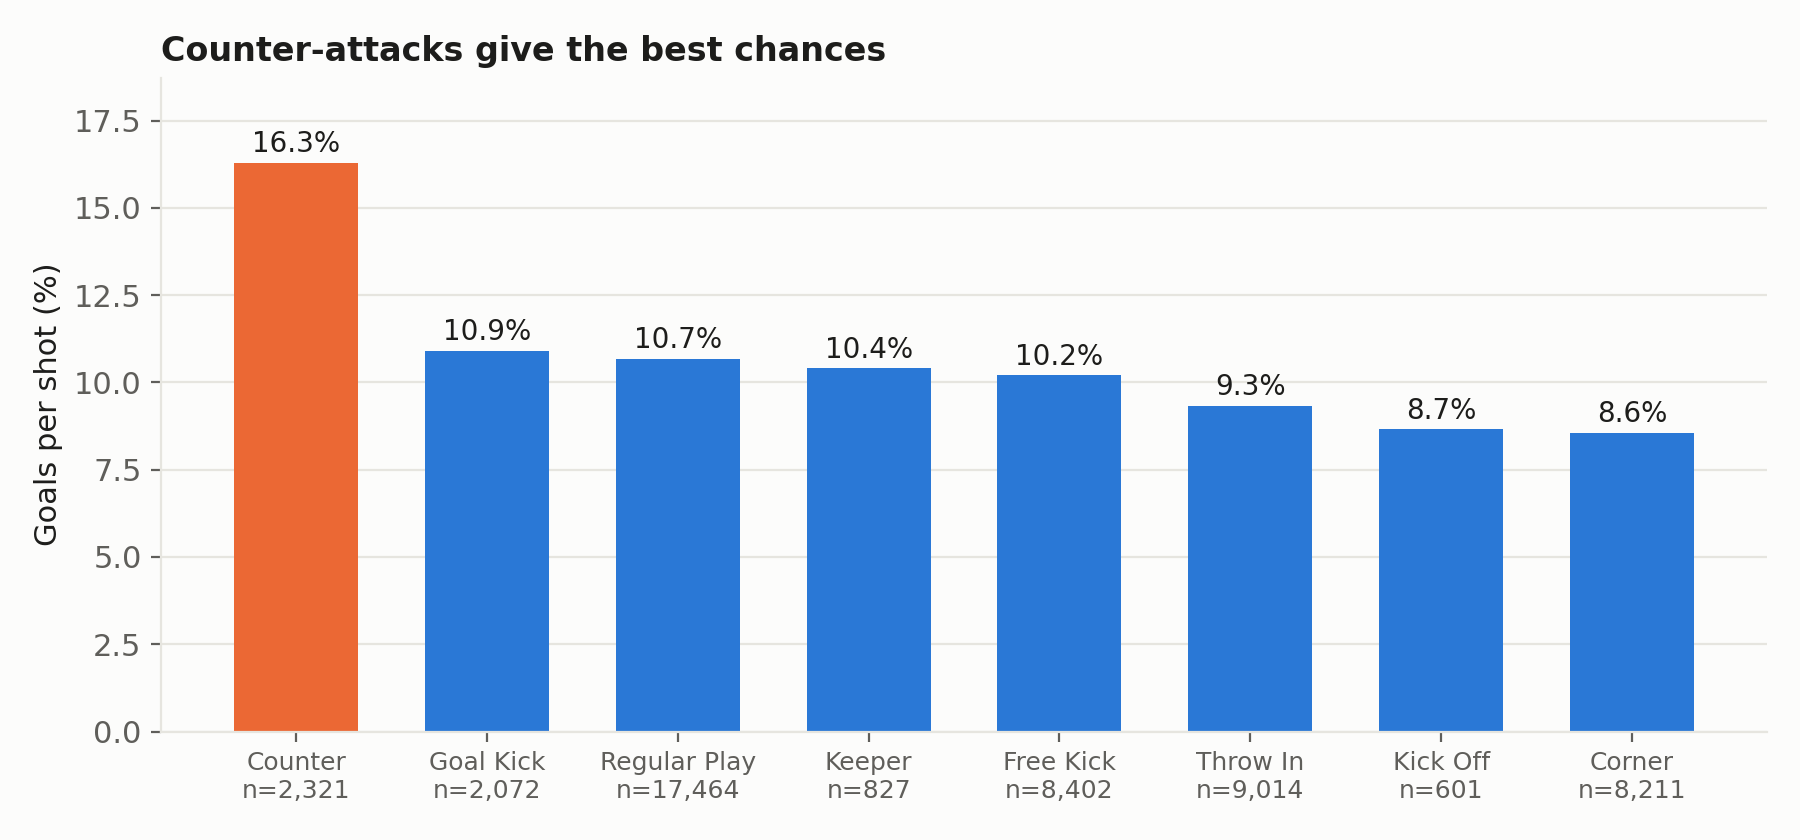
\includegraphics[width=0.9\textwidth]{images/playpattern.png}
    \caption{Goal Percentage by Play Pattern}
    \label{playpattern}
\end{figure}

Counter attacks stand out (figure \ref{playpattern}): 16.3\% of shots from counters were goals, against 8.6\%--10.9\% for every other pattern. Shots after corners and kick-offs converted least often (8.6\% and 8.7\%). The original edition stated that many goals came from kick-offs; on the wider data this does not hold, and kick-offs lead to few shots (1.2\%) that convert below average.

Following the original study, the model uses play pattern in two groups, Regular Play and Non Regular Play. Their goal rates differ little (10.7\% and 10.0\%), because the grouping mixes counters with corners. This is one of the reasons the play pattern ends up as the least useful feature (section \ref{res:importance}), and a finer grouping that keeps counter attacks apart is suggested as future work.

\newpage

\subsection{Pass Type and Ball Height}

The key pass before a shot can be a ground pass, a low pass (in the air, below shoulder height) or a high pass. Some shots follow no pass at all, for example after a dribble or a rebound. The hypothesis was that ground and low passes lead to better chances than high passes.

\begin{figure}[!h]
    \centering
    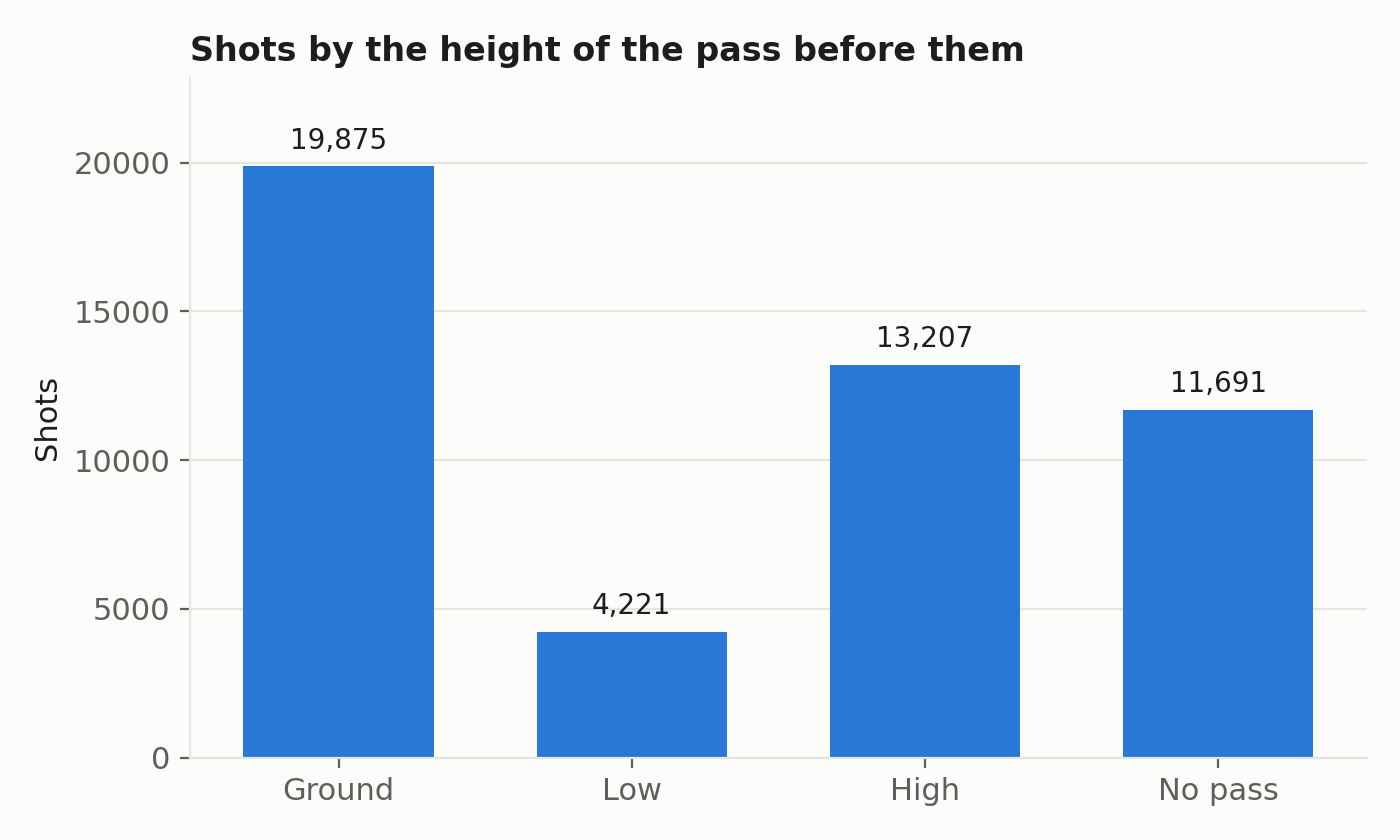
\includegraphics[width=0.7\textwidth]{images/passtypeshot.png}
    \caption{Shots by Pass Type}
    \label{passtypeshot}
\end{figure}

Ground passes and high passes created the most shots (figure \ref{passtypeshot}). High passes lead to shots much closer to goal, with a median of 11.4 yards against 21.7 yards after a ground pass (figure \ref{passtypebox}), because 57\% of the shots after a high pass are headers.

\begin{figure}[!h]
    \centering
    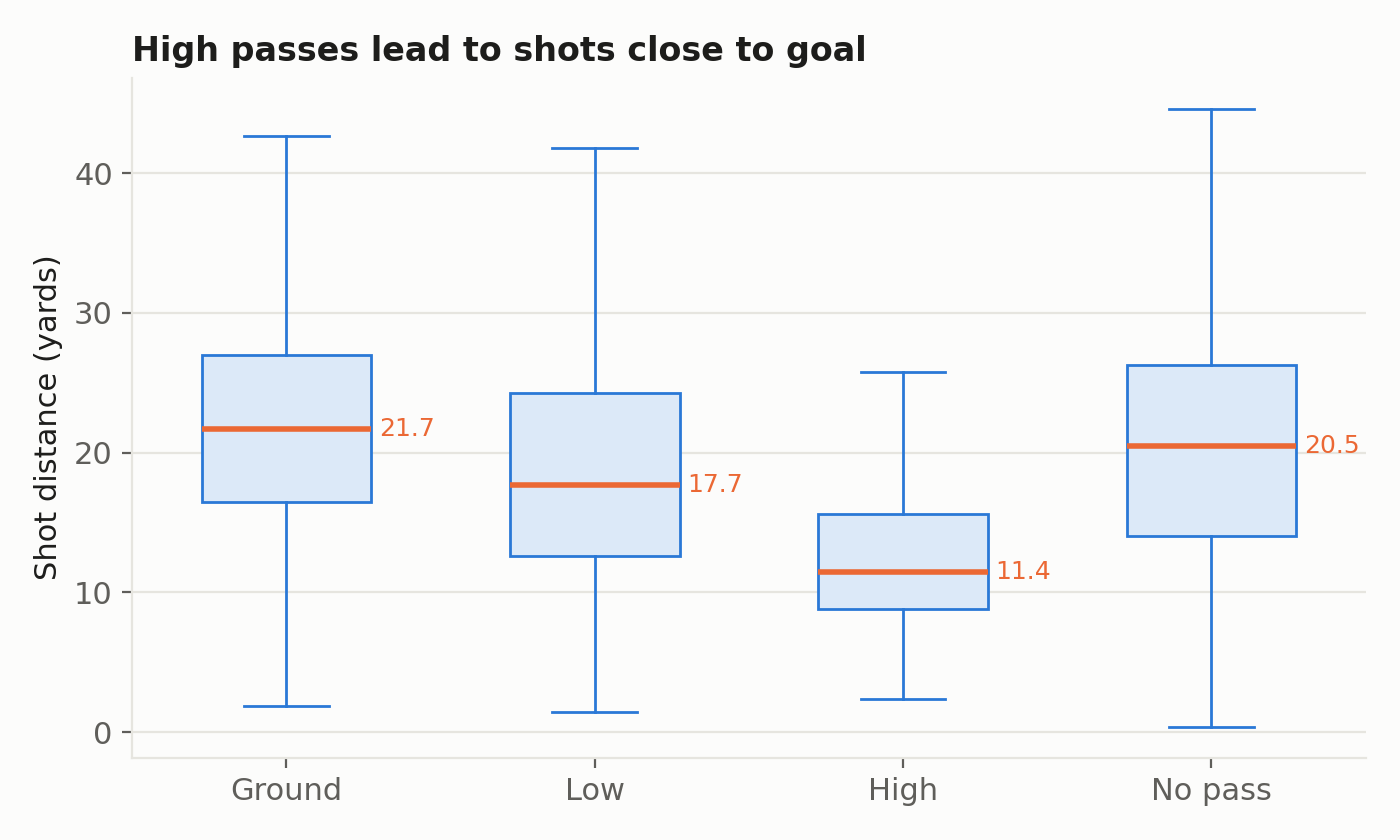
\includegraphics[width=0.7\textwidth]{images/passtypebox.png}
    \caption{Shot Distance by Pass Type (box plots without outliers)}
    \label{passtypebox}
\end{figure}

Over all distances, the goal rates differ little: 9.7\% after a ground pass, 11.9\% after a low pass, 10.3\% after a high pass and 10.5\% with no pass. At the same distance, the hypothesis holds clearly (figure \ref{passtypeperc}). Under 12 yards, 37.5\% of shots after a ground pass were goals, but only 13.7\% of shots after a high pass. The ball arriving in the air, and often having to be headed, makes the chance much harder.

\begin{figure}[!h]
    \centering
    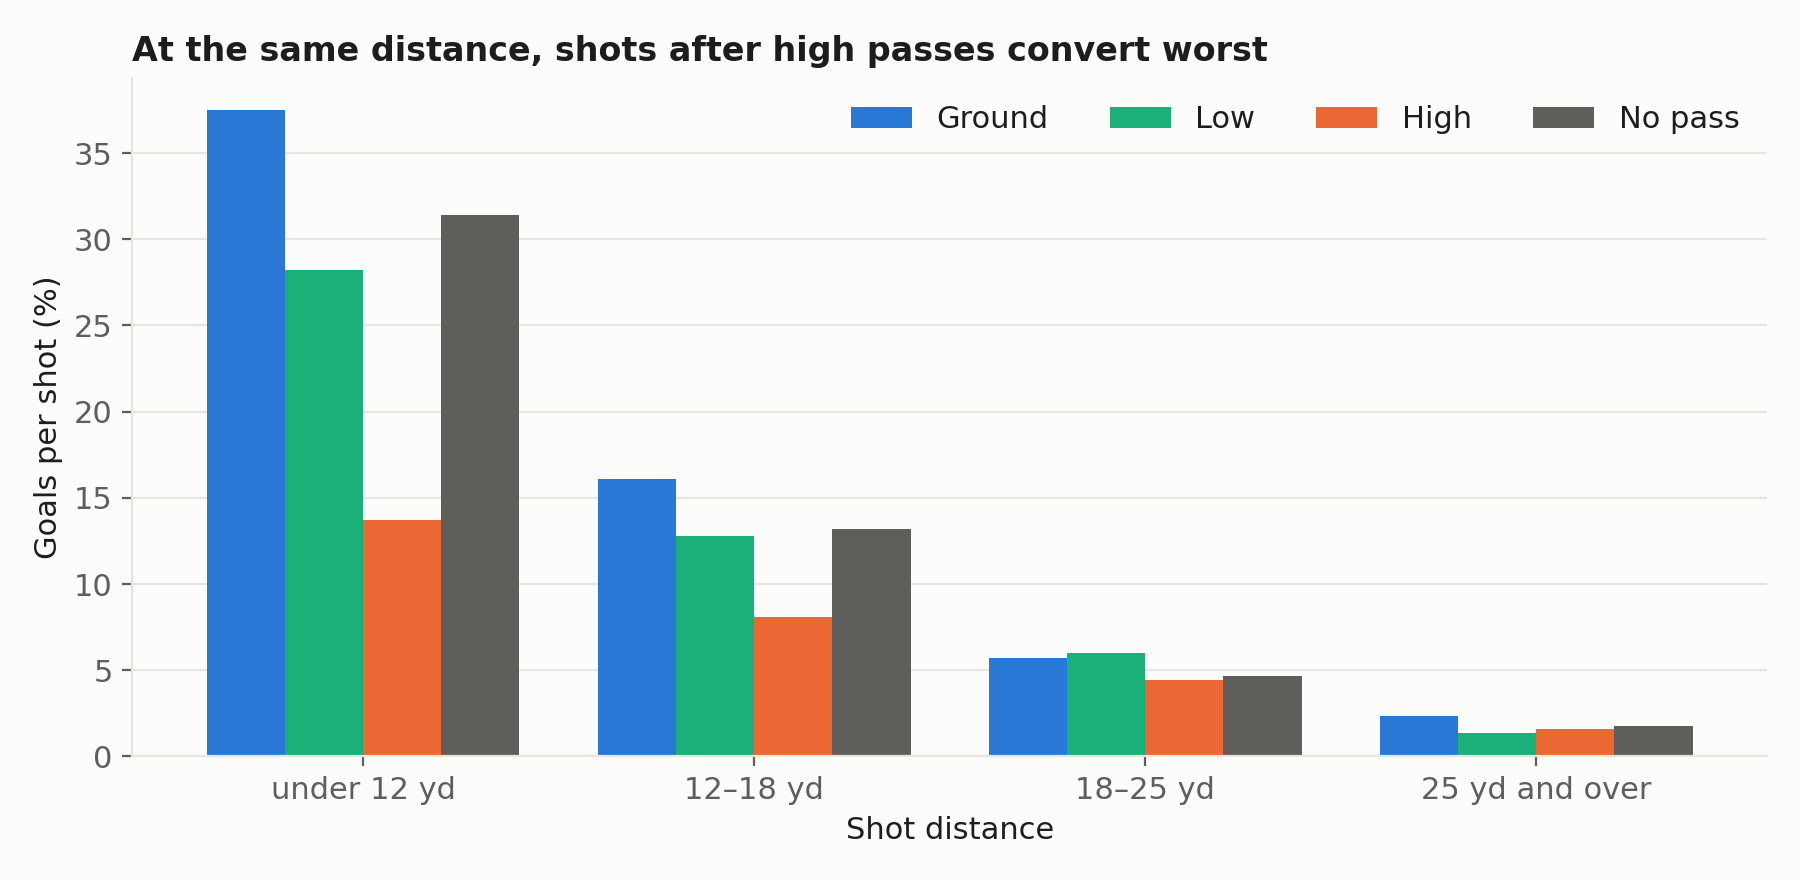
\includegraphics[width=0.9\textwidth]{images/passtypeperc.png}
    \caption{Goal Percentage by Pass Type within Distance Bands}
    \label{passtypeperc}
\end{figure}

\newpage

\subsection{Direct Goals From Set Pieces}

A set piece restarts play after a foul or after the ball has gone out of play: corners, free kicks and penalties \cite{washington}. Shots taken directly from a free kick or a penalty are very different chances from open-play shots. Penalties are usually given a fixed xG of about 0.76--0.79, and direct free kicks are modelled separately. This model therefore covers open-play shots only.

\subsection{First Time Shot}

A first-time shot is struck with the player's first touch, giving the defence and the goalkeeper less time to react. The hypothesis was that first-time shots have a higher xG, and it held: 14.0\% of first-time shots were goals against 8.4\% of the others (figure \ref{firstime}). The difference is largest close to goal: under 12 yards, 31.3\% against 16.0\%.

\begin{figure}[!h]
    \centering
    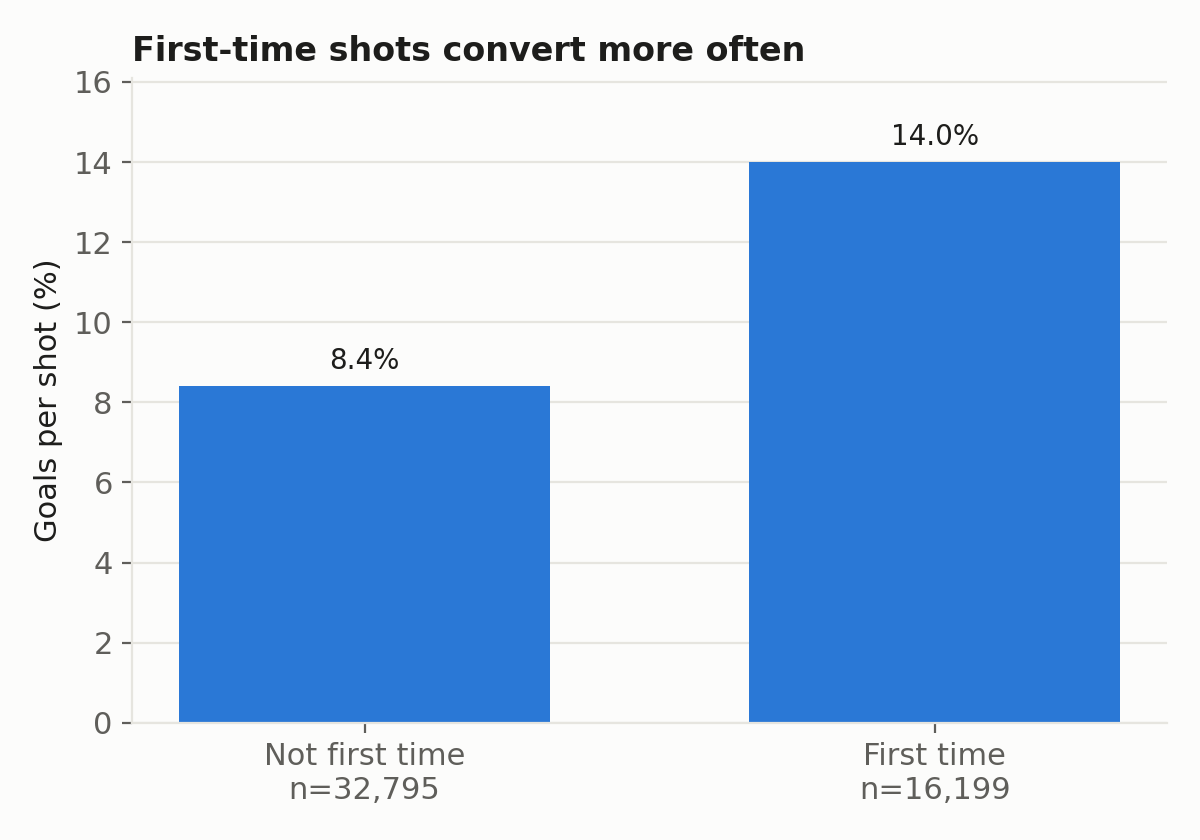
\includegraphics[width=0.6\textwidth]{images/firsttimeperc.png}
    \caption{Goals vs First Time Shots}
    \label{firstime}
\end{figure}

\newpage

\subsection{Technique Used and Shot Velocity}

The technique used to strike the ball, and the speed of the shot, say a lot about shot quality. Both were left out of the model on purpose. Expected Goals measures the quality of a chance \textbf{before} the shot is taken (\textbf{pre-shot analysis}), and the technique and speed of a shot are part of how the chance was taken, not of the chance itself. Their use in post-shot models is discussed in section \ref{future}.

\begin{figure}[!h]
    \centering
    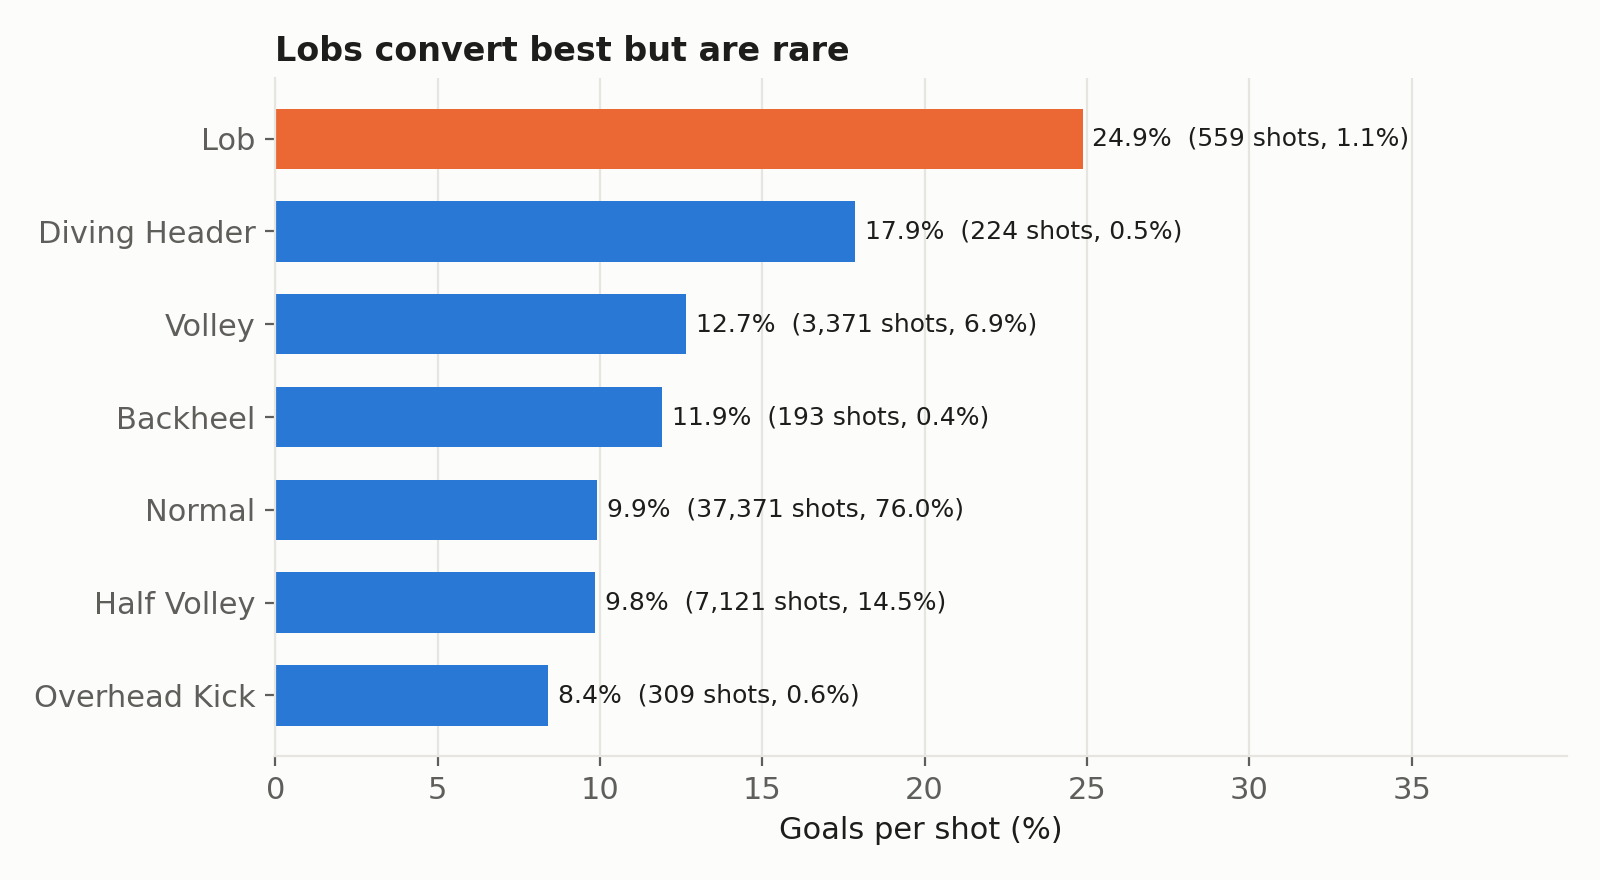
\includegraphics[width=0.9\textwidth]{images/tech.png}
    \caption{Goal Percentage by Shot Technique}
    \label{tech}
\end{figure}

Figure \ref{tech} shows that the lob had the highest conversion: 24.9\% of lobbed shots were goals, about one in four. Lobs are attempted only in particular situations, such as when the goalkeeper has come off the line, and they made up only 1.1\% of the open-play shots. Normal strikes were 76\% of shots and converted at 9.9\%.

With this, the Exploratory Data Analysis was concluded.

\newpage

\section{Feature Engineering}\label{feature}

Feature Engineering is the process of building new features from the existing data to improve predictive modelling. The features below were engineered from the raw shot data and the freeze frames. Section \ref{EDA} covered how each of them relates to goals.

\begin{itemize}
    \item Number of opponents in 5 yards: the number of opponents within 5 yards of the shooter
    \item Players between goal: the number of opponents, including the goalkeeper, inside the triangle formed by the ball and the two goal posts
    \item Shot Distance: the distance from the ball to the centre of the goal
    \item Goalkeeper Distance: the distance from the goalkeeper to the centre of the goal
    \item Shot Angle: the angle at the ball between the lines to the two goal posts
    \item Goal: the target, 1 for a goal and 0 otherwise
\end{itemize}

Each of these features can be seen in figure \ref{example}.

\newpage

\subsection{Mathematical Concepts Used}

As highlighted in \cite{maor2019pythagorean}, the distance formula gives the distance between any two points:

\begin{equation}
d = \sqrt{(x_2-x_1)^2 + (y_2-y_1)^2}
\label{distance}
\end{equation}

where $x_1, y_1$ and $x_2, y_2$ are the coordinates of the two points. The shot distance, for example, is the distance from the shot location to the centre of the goal at $(120, 40)$.

To calculate the Shot Angle, the Law of Cosines \cite{heath1956thirteen} was applied to the triangle formed by the ball and the two posts:

\begin{equation}
    c^2 = a^2 + b^2 - 2ab\cos\theta
    \label{law}
\end{equation}

where $a$ and $b$ are the distances from the ball to each goal post, $c$ is the distance between the posts (8 yards), and $\theta$ is the shot angle. An example can be seen in figure \ref{example}, where the red lines are $a$ and $b$. Rearranged, equation \ref{law} gives the shot angle:

\begin{equation}
\theta = \arccos\left(\frac{a^2 + b^2 - c^2}{2ab}\right)
\end{equation}

\begin{figure}[!h]
    \centering
    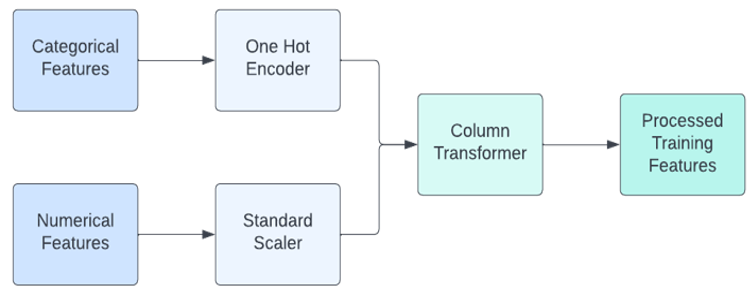
\includegraphics[scale=0.7]{images/featurepipe.png}
    \caption{Feature Processing}
    \label{featurepipe}
\end{figure}

\subsection{Final Features}

The model uses 13 features, the same as in the original edition:
\begin{itemize}
    \item 4 categorical features: body part (foot or head), pass type (ground, low, high or none), play pattern (regular or non-regular play) and first time (yes or no)
    \item 9 numerical features: shot distance, shot angle, opponents within 5 yards, players between the ball and goal, the x and y coordinates of the shot, goalkeeper distance, and the x and y coordinates of the goalkeeper
\end{itemize}

The two kinds of feature need different treatment before Machine Learning. Categorical features were one-hot encoded and numerical features were standardised, using the One Hot Encoder, Standard Scaler and Column Transformer of the Scikit-Learn library \cite{scikit-learn} (figure \ref{featurepipe}). After encoding, the 13 features become 19 model inputs. The encoder ignores categories it has not seen in training, so a rare category in new data cannot break the model.

\newpage

\section{Model Tuning and Evaluation}\label{test}

\subsection{Algorithms}

Four algorithms were used to predict xG:

\begin{itemize}
    \item Logistic Regression
    \item XGBoost
    \item LightGBM
    \item CatBoost
\end{itemize}

\subsubsection{Logistic Regression}
Logistic Regression is widely used for classification and predictive analytics. Based on a set of independent variables, it estimates the probability of an event, such as a goal. The log of the odds (the probability of success divided by the probability of failure) is modelled as a linear function of the features, so the output always lies between 0 and 1 \cite{1194264}.

\subsubsection{LightGBM}
LightGBM is a gradient boosting toolkit using tree-based learning, developed by Microsoft \cite{ke2017lightgbm}. It is designed to be fast and efficient:

\begin{itemize}
    \item Fast training and low memory use.
    \item Support for parallel, distributed and GPU learning.
    \item Able to handle large amounts of data.
\end{itemize}

\subsubsection{XGBoost}
XGBoost is a distributed gradient boosting library designed to be efficient, flexible and portable. It builds an ensemble of decision trees, each correcting the errors of the previous ones, and provides parallel tree boosting for a wide range of problems \cite{Chen:2016:XST:2939672.2939785}.

\subsubsection{CatBoost}
CatBoost is a gradient boosting library developed by Yandex. It builds symmetric trees and uses ordered boosting, which reduces overfitting, and it handles categorical data well \cite{DBLP:journals/corr/DorogushGGKPV17}.

\subsection{Splitting the Data by Match}

Shots from the same match are not independent: they share the same teams, the same conditions and often the same passage of play. If shots from one match are in both the training and the test set, the test result is too optimistic. The data was therefore split by \textbf{match}: 20\% of the matches (524 matches, 12,009 shots) were held out as the test set, and the models were trained on the other 2,092 matches (48,994 shots). No match has shots on both sides. The original edition split individual shots at random, so its test set shared matches with its training set.

\subsection{Hyper-Parameter Tuning}

Hyper-parameter tuning searches for the settings that make a model perform best \cite{hyperparameter}. Each model's settings were chosen with Randomized Search with cross-validation (RandomizedSearchCV in Scikit-Learn \cite{scikit-learn}) on the training matches only:
\begin{itemize}
    \item 5-fold cross-validation, with the folds also grouped by match
    \item 20 settings tried for Logistic Regression, XGBoost and LightGBM, and 12 for CatBoost, which is slower to train
    \item settings scored by \textbf{log loss}, because xG must be a good probability, not only a good ranking of shots
\end{itemize}

The settings searched were:
\begin{itemize}
    \item Logistic Regression: the regularisation strength $C$
    \item Tree models: the depth of the trees (or number of leaves), the number of trees, the learning rate, the L2 regularisation, and for XGBoost and LightGBM the share of rows and columns used for each tree and the minimum size of a leaf
\end{itemize}

The model with the best cross-validated log loss was chosen as the final model before the test set was used. The test set was used once, to report the results in chapter \ref{results}.

\subsection{Evaluation Metrics}

An xG value is a probability, and xG totals are used to judge players and teams. A good xG model must therefore not only rank shots well; its probabilities must also match how often goals are actually scored. Each model was evaluated on:
\begin{itemize}
    \item \textbf{Log loss}: how close the predicted probabilities are to the outcomes (1 for a goal, 0 otherwise). Lower is better. It punishes confident wrong predictions heavily, and it is the main measure used in this study. For reference, always predicting the average goal rate of 10.3\% gives a log loss of about 0.33.
    \item \textbf{Brier score}: the mean squared difference between the predicted probability and the outcome. Lower is better.
    \item \textbf{AUC}: the area under the ROC curve, the probability that a randomly chosen goal gets a higher xG than a randomly chosen miss. Higher is better; 0.5 is guessing. AUC measures ranking only, so a model can have a good AUC and still predict far too many or too few goals.
    \item \textbf{Calibration error (ECE)}: the shots are split into 10 equal-size groups by predicted xG, and in each group the mean xG is compared with the actual share of goals. ECE is the average gap, weighted by group size. Lower is better.
    \item \textbf{Predicted ÷ actual goals}: the total xG divided by the number of goals. 1.00 is perfect; above 1 means the model predicts too many goals.
\end{itemize}

StatsBomb's own xG, available for every shot, was evaluated on the same shots as a reference point.

\subsection{Out-of-Fold xG for Team and Player Analysis}

To analyse teams and players (section \ref{res:teams}), every shot needs an xG from a model that has not seen it. The final model was therefore also trained 5 times, each time on 80\% of the matches, and used to predict the other 20\%. Every one of the 61,003 shots gets an xG from a model that never saw its match. These \textit{out-of-fold} predictions are used for all team and player tables.

\chapter{Results}\label{results}

This chapter reports the four models on the 524 held-out matches (section \ref{res:models}), the features they rely on (section \ref{res:importance}), what the model says about teams and players (section \ref{res:teams}), and whether one model can serve different leagues (section \ref{res:leagues}).

\section{Model Validation}\label{res:models}

Table \ref{tab:models} shows the results of the four tuned models on the held-out test matches: 12,009 open-play shots and 1,253 goals. StatsBomb's own xG for the same shots is included as a reference point.

\begin{table}[!h]
\centering
\small
\begin{tabular}{|l|c|c|c|c|c|c|}
\hline
\textbf{Model} & \textbf{CV log loss} & \textbf{Log loss} & \textbf{Brier} & \textbf{AUC} & \textbf{ECE} & \textbf{xG ÷ goals} \\
\hline
Logistic Regression & 0.2655 & 0.2699 & 0.0776 & 0.804 & 0.0047 & 1.00 \\
XGBoost & 0.2640 & 0.2686 & 0.0771 & 0.806 & 0.0058 & 0.99 \\
LightGBM & 0.2642 & 0.2696 & 0.0774 & 0.804 & 0.0065 & 0.99 \\
\textbf{CatBoost} & \textbf{0.2637} & 0.2687 & 0.0772 & 0.806 & 0.0048 & 0.99 \\
\hline
StatsBomb xG & -- & 0.2647 & 0.0759 & 0.813 & 0.0101 & 0.94 \\
\hline
\end{tabular}
\caption{Results on 524 held-out matches. CV log loss is the cross-validated log loss on the training matches, used to choose the final model.}
\label{tab:models}
\end{table}

\textbf{CatBoost} had the best cross-validated log loss and was chosen as the final model, before the test set was used. Its tuned settings were a tree depth of 7, 302 trees, a learning rate of 0.025 and an L2 regularisation of 4.56. The tuned Logistic Regression used $C = 0.144$.

\subsection{The Choice of Algorithm barely Matters}

The four models are almost tied. On the test matches, their log loss differs by at most 0.0013 and their AUC by 0.002, and their ROC curves lie on top of each other (figure \ref{fig:roc}). To check whether the differences are real, the test matches were resampled 2,000 times (a match bootstrap, so that shots from one match stay together). CatBoost's log loss was 0.0012 lower than Logistic Regression's, but the 95\% interval ($-0.0029$ to $+0.0004$) includes zero, so the simplest model cannot be said to be worse. CatBoost was indistinguishable from XGBoost, and slightly but clearly better than LightGBM (by 0.0010; interval $-0.0018$ to $-0.0001$).

\begin{figure}[!h]
    \centering
    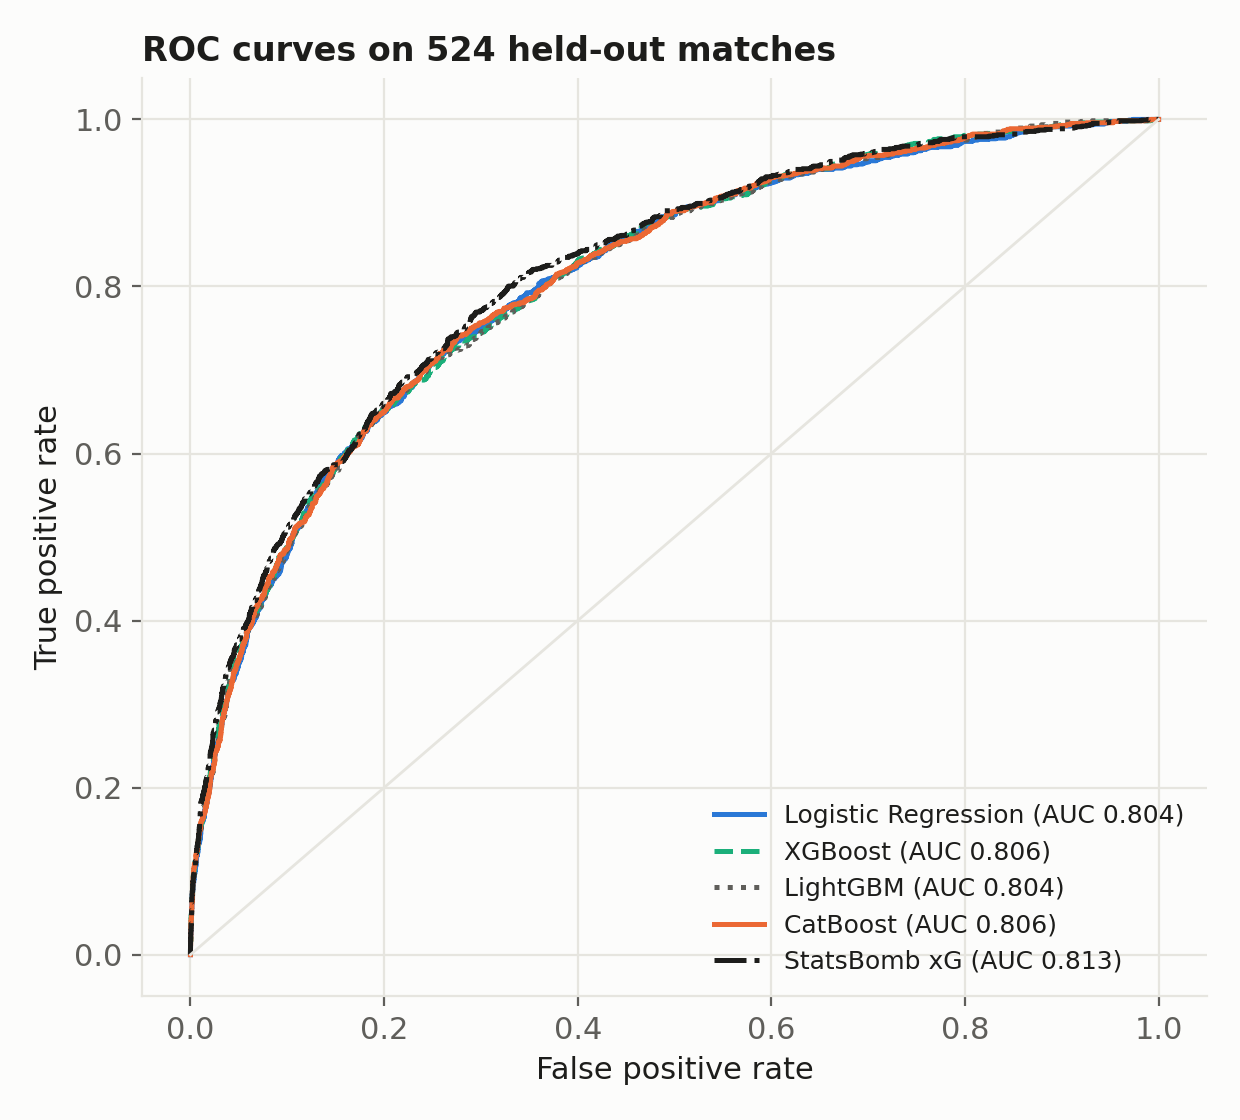
\includegraphics[width=0.65\textwidth]{images/roc.png}
    \caption{ROC Curves on the Held-out Matches}
    \label{fig:roc}
\end{figure}

\subsection{Predictions match Reality}

All four models are well calibrated. Their calibration error is about half a percentage point, and they predict between 98.7\% and 99.6\% of the goals actually scored in the test matches; the 95\% intervals, roughly $\pm$4.5\%, all include 100\%. Figure \ref{fig:calibration} shows the calibration of CatBoost: in each group of shots, from the least to the most promising, the mean xG is close to the share of goals.

\begin{figure}[!h]
    \centering
    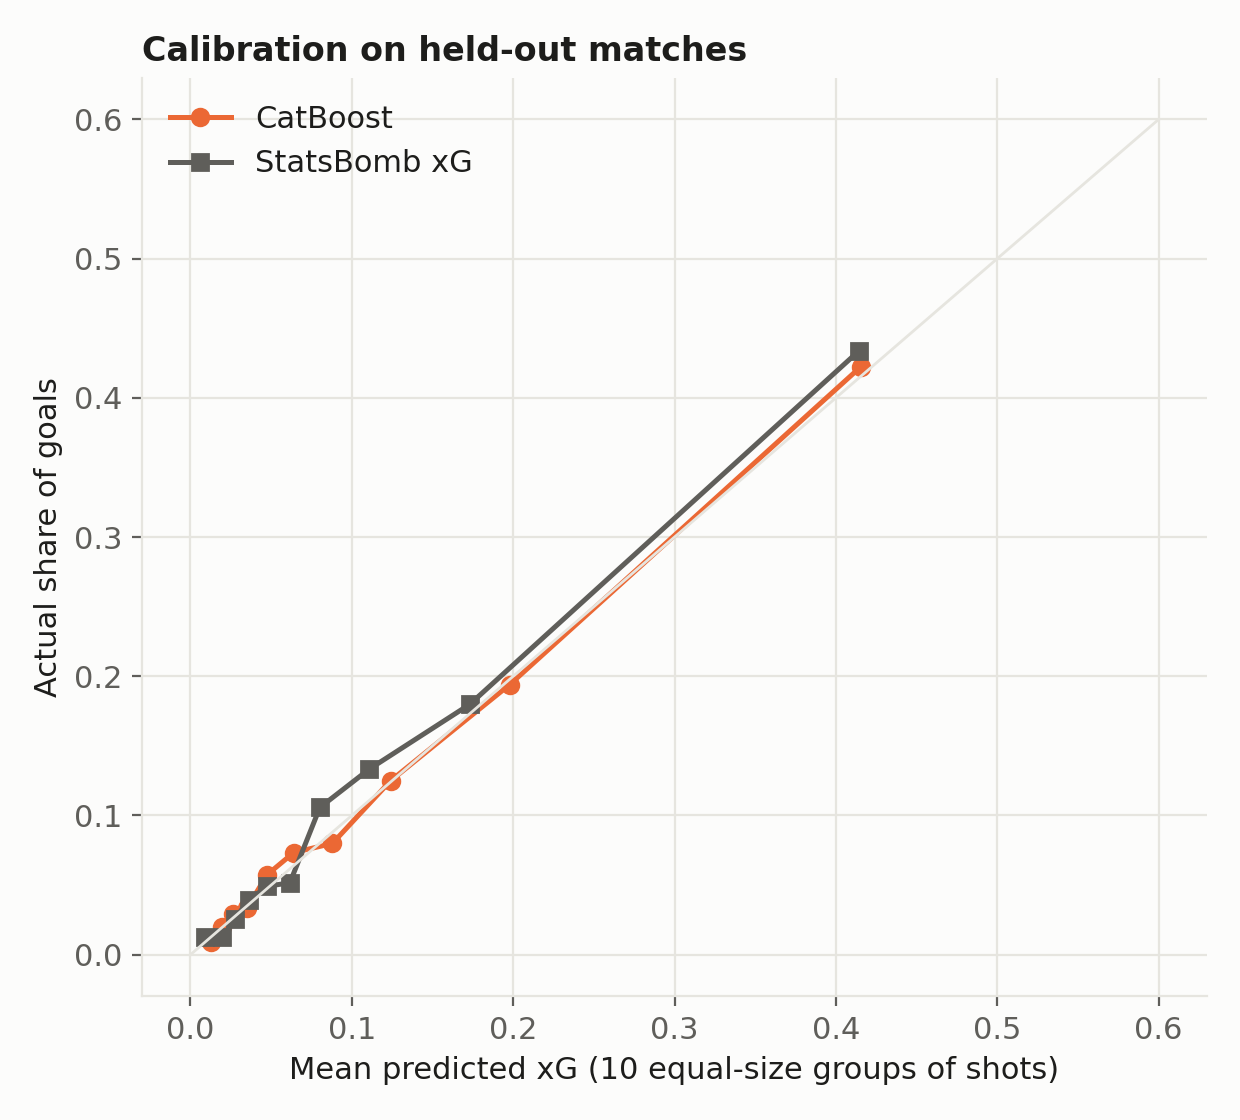
\includegraphics[width=0.65\textwidth]{images/calibration.png}
    \caption{Calibration on the Held-out Matches}
    \label{fig:calibration}
\end{figure}

\subsection{Comparison with StatsBomb xG}

StatsBomb's xG scores better on log loss (by 0.0039; interval 0.0018 to 0.0061) and AUC (0.813 against 0.806). It is a reference point rather than a fair competitor: StatsBomb trains its model on far more data and on information beyond these 13 features, very likely including these same matches. StatsBomb's xG is less well calibrated on these matches, however: it predicts 6\% fewer goals than were scored (0.94; interval 0.90 to 0.98).

\subsection{Comparison with the Original Edition}

The original edition reported AUC scores between 0.80 and 0.82, against 0.84 for StatsBomb. Those scores were measured on Barcelona's matches, with shots from the same match on both sides of a random split. The scores here (0.804--0.806) are measured on unseen matches from many competitions. They are a harder and fairer test, not a drop in quality.

Every shot also has an out-of-fold xG from a model that never saw its match (section \ref{test}). Across all 61,003 shots these have a log loss of 0.2645, an AUC of 0.809 and a calibration error of 0.003, and they predict 99.7\% of the goals scored.

\newpage

\section{Feature Importance}\label{res:importance}

To see which features each model relies on, every feature was shuffled in turn on the test matches, which breaks its link with the outcome, and the increase in log loss was measured (permutation importance, averaged over 5 shuffles). Figure \ref{fig:importance} shows the result for Logistic Regression and CatBoost.

\begin{figure}[!h]
    \centering
    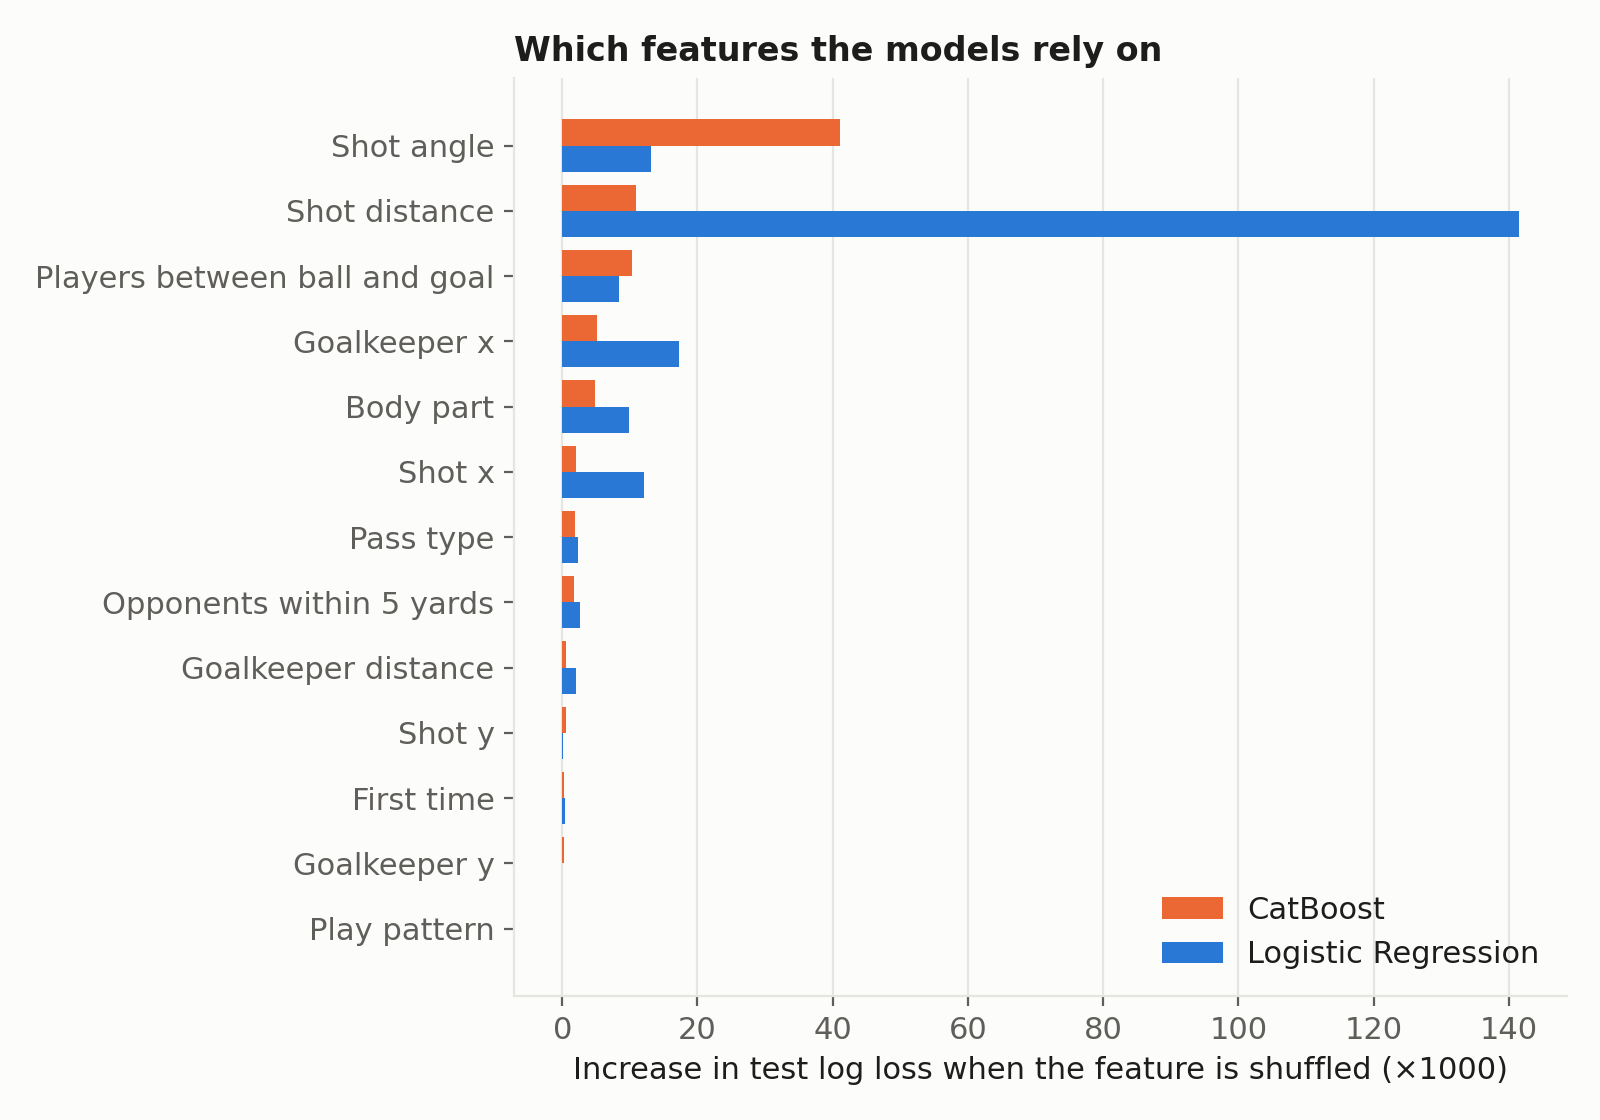
\includegraphics[width=0.9\textwidth]{images/importance.png}
    \caption{Permutation Importance on the Held-out Matches}
    \label{fig:importance}
\end{figure}

Both models rely on the geometry of the shot, but they divide the credit differently:
\begin{itemize}
    \item \textbf{Logistic Regression} relies above all on shot distance (an increase of 0.142 in log loss when it is shuffled), followed by the goalkeeper's x coordinate, shot angle, the shot's x coordinate, body part and the players between the ball and goal.
    \item \textbf{CatBoost} relies most on shot angle (0.041), followed by shot distance and the players between the ball and goal (0.011 and 0.010), then the goalkeeper's x coordinate and body part (0.005 each).
\end{itemize}

The difference is a consequence of how the two models work, not a disagreement about football. Shot distance, shot angle and the shot's x coordinate carry much of the same information. A linear model needs distance to describe how the chance falls away from goal, while the trees of CatBoost can take the same information from the angle. When features overlap, permutation importance shares the credit between them in a way that depends on the model, so the ranking within this group should not be read too literally.

The features that matter little are clearer. Pressure, pass type, goalkeeper distance and the shot's y coordinate add a little. First time and the goalkeeper's y coordinate add almost nothing once the rest is known, and play pattern adds nothing at all in either model. As discussed in the exploratory analysis, grouping the play patterns into Regular and Non Regular Play hides the one pattern that stands out, the counter attack.

\newpage

\section{Teams and Players}\label{res:teams}

The tables in this section use the out-of-fold xG, so each shot's xG comes from a model that never saw its match. They count open-play shots and goals only, the shots the model covers; penalties, direct free kicks and own goals are not included, so ``goals'' here is lower than official totals.

\subsection{League Tables 2015/16}

StatsBomb's open data contains the full 2015/16 seasons of the Premier League, La Liga and Serie A, and all but 3 matches of Ligue 1. The points and positions calculated from the match results match the official final tables exactly for the first three leagues. Table \ref{tab:spearman} shows how well each team's xG difference (xG for minus xG against) tracks its points.

\begin{table}[!h]
\centering
\begin{tabular}{|l|c|c|c|}
\hline
\textbf{League} & \textbf{Matches} & \textbf{xG diff. vs points} & \textbf{Goal diff. vs points} \\
\hline
Premier League & 380 & 0.85 & 0.93 \\
La Liga & 380 & 0.73 & 0.85 \\
Serie A & 380 & 0.83 & 0.95 \\
Ligue 1 & 377 & 0.61 & 0.65 \\
\hline
\end{tabular}
\caption{Rank correlation (Spearman) of open-play xG difference and open-play goal difference with points, 2015/16}
\label{tab:spearman}
\end{table}

xG difference tracks the table well, though less closely than actual goal difference. That is expected, since points are decided by actual goals. xG measures the quality of the chances a team created and allowed, and the gap between the two shows which teams did better or worse than their chances.

The 2015/16 Premier League is a famous example (figure \ref{fig:pl} and table \ref{tab:pl}). Leicester City won the league with 81 points while ranking only 6th on open-play xG difference; among other things, they conceded 32 open-play goals from chances worth 44.6 xG. Arsenal had the best xG difference in the league (+34.1) and finished second, 10 points behind. Aston Villa were last on both measures.

\begin{figure}[!h]
    \centering
    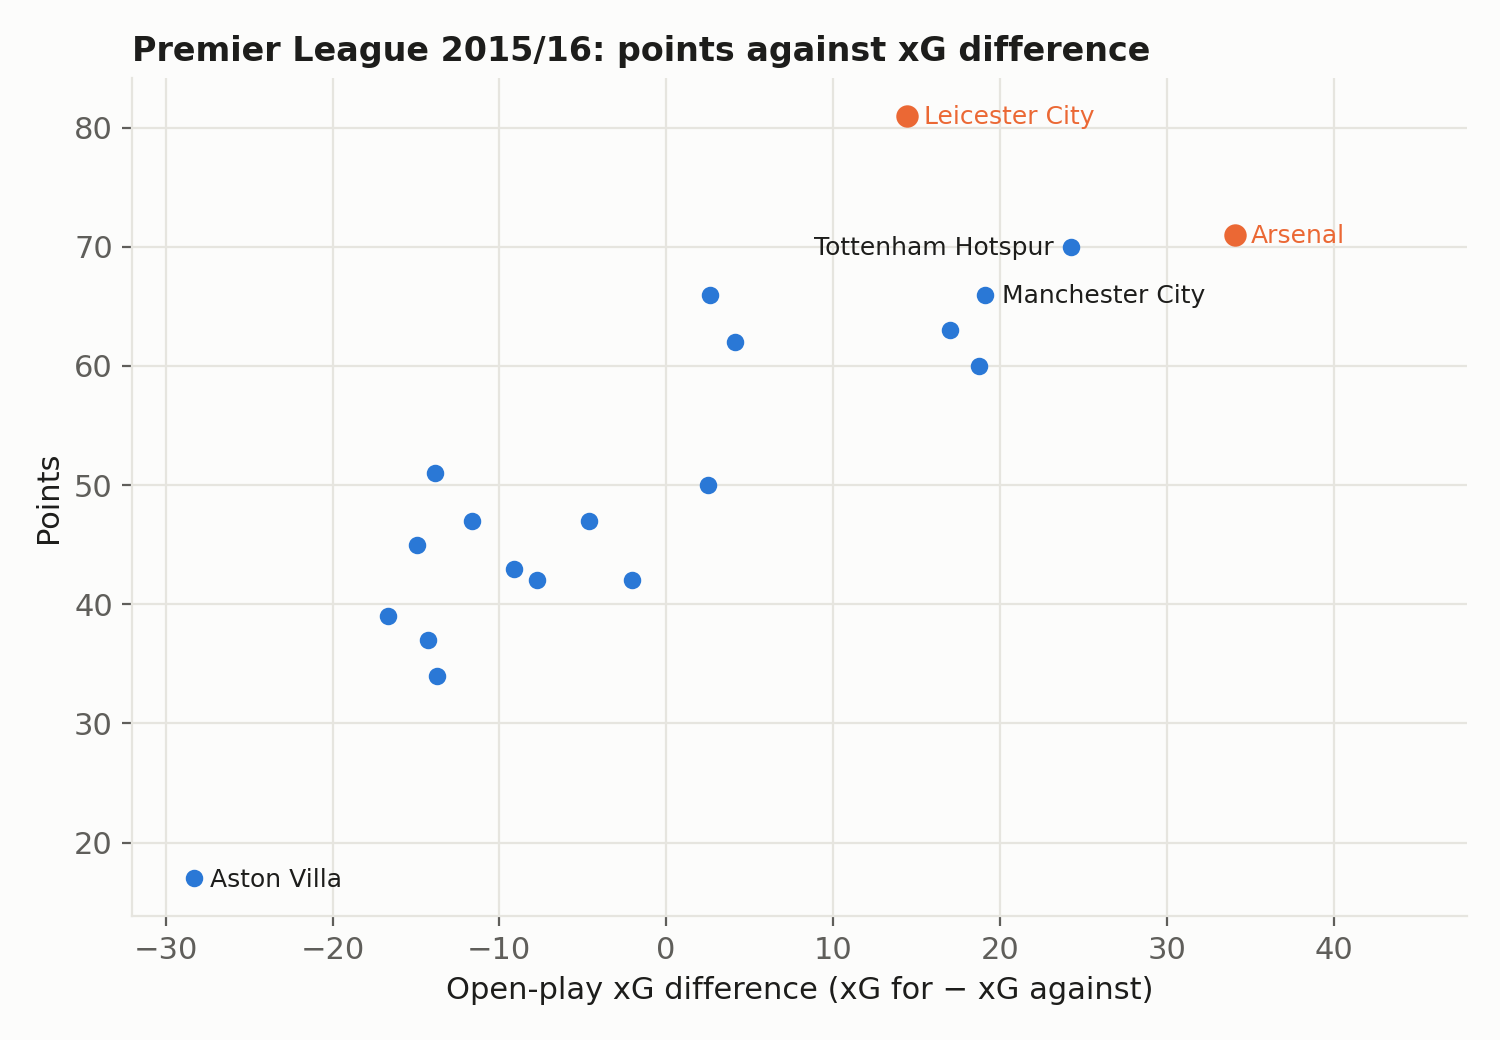
\includegraphics[width=0.8\textwidth]{images/pl_2015_16.png}
    \caption{Premier League 2015/16: Points against Open-play xG Difference}
    \label{fig:pl}
\end{figure}

\begin{table}[!h]
\centering
\small
\begin{tabular}{|c|l|c|c|c|c|c|c|c|}
\hline
\textbf{Pos} & \textbf{Team} & \textbf{Pts} & \textbf{GF} & \textbf{xGF} & \textbf{GA} & \textbf{xGA} & \textbf{xG diff} & \textbf{xG rank} \\
\hline
1 & Leicester City & 81 & 56 & 59.0 & 32 & 44.6 & 14.4 & 6 \\
2 & Arsenal & 71 & 61 & 68.8 & 30 & 34.8 & 34.1 & 1 \\
3 & Tottenham Hotspur & 70 & 60 & 59.7 & 31 & 35.4 & 24.2 & 2 \\
4 & Manchester City & 66 & 62 & 58.6 & 39 & 39.4 & 19.1 & 3 \\
5 & Manchester United & 66 & 42 & 40.7 & 29 & 38.1 & 2.6 & 8 \\
6 & Southampton & 63 & 53 & 54.7 & 37 & 37.6 & 17.0 & 5 \\
7 & West Ham United & 62 & 57 & 53.4 & 40 & 49.2 & 4.2 & 7 \\
8 & Liverpool & 60 & 57 & 56.8 & 48 & 38.0 & 18.8 & 4 \\
9 & Stoke City & 51 & 35 & 37.6 & 48 & 51.5 & -13.8 & 16 \\
10 & Chelsea & 50 & 47 & 51.4 & 47 & 48.9 & 2.5 & 9 \\
11 & Everton & 47 & 50 & 50.0 & 49 & 54.6 & -4.6 & 11 \\
12 & Swansea City & 47 & 32 & 39.1 & 40 & 50.7 & -11.6 & 14 \\
13 & Watford & 45 & 30 & 38.3 & 42 & 53.2 & -15.0 & 18 \\
14 & West Bromwich Albion & 43 & 29 & 36.0 & 37 & 45.2 & -9.1 & 13 \\
15 & Crystal Palace & 42 & 34 & 40.9 & 39 & 48.6 & -7.7 & 12 \\
16 & AFC Bournemouth & 42 & 40 & 41.6 & 60 & 43.6 & -2.1 & 10 \\
17 & Sunderland & 39 & 35 & 38.8 & 55 & 55.5 & -16.7 & 19 \\
18 & Newcastle United & 37 & 39 & 39.5 & 57 & 53.8 & -14.3 & 17 \\
19 & Norwich City & 34 & 36 & 40.0 & 58 & 53.8 & -13.7 & 15 \\
20 & Aston Villa & 17 & 24 & 29.4 & 61 & 57.7 & -28.3 & 20 \\
\hline
\end{tabular}
\caption{Premier League 2015/16 with open-play goals (GF, GA) and xG (xGF, xGA)}
\label{tab:pl}
\end{table}

In La Liga, the top three (Barcelona, Real Madrid and Atlético Madrid) were also the top three on xG difference, while Villarreal finished 4th with only the 11th best xG difference. In Serie A, Napoli had a slightly better xG difference than the champions Juventus. The full tables for all four leagues are in the project repository (\texttt{docs/TABLES.md}).

\newpage

\subsection{Finishing: Goals against xG}

xG describes how good a player's chances were; comparing it with the goals the player actually scored shows how well the chances were taken. Because luck plays a large part, the gap is also expressed as a $z$ score: the difference between goals and xG divided by how much that difference would vary by chance for an average finisher taking the same shots,
\begin{equation}
z = \frac{\text{goals} - \sum_i p_i}{\sqrt{\sum_i p_i(1 - p_i)}}
\end{equation}
where $p_i$ is the xG of each shot. Roughly, a $|z|$ above 2 is unlikely to be luck alone.

\begin{figure}[!h]
    \centering
    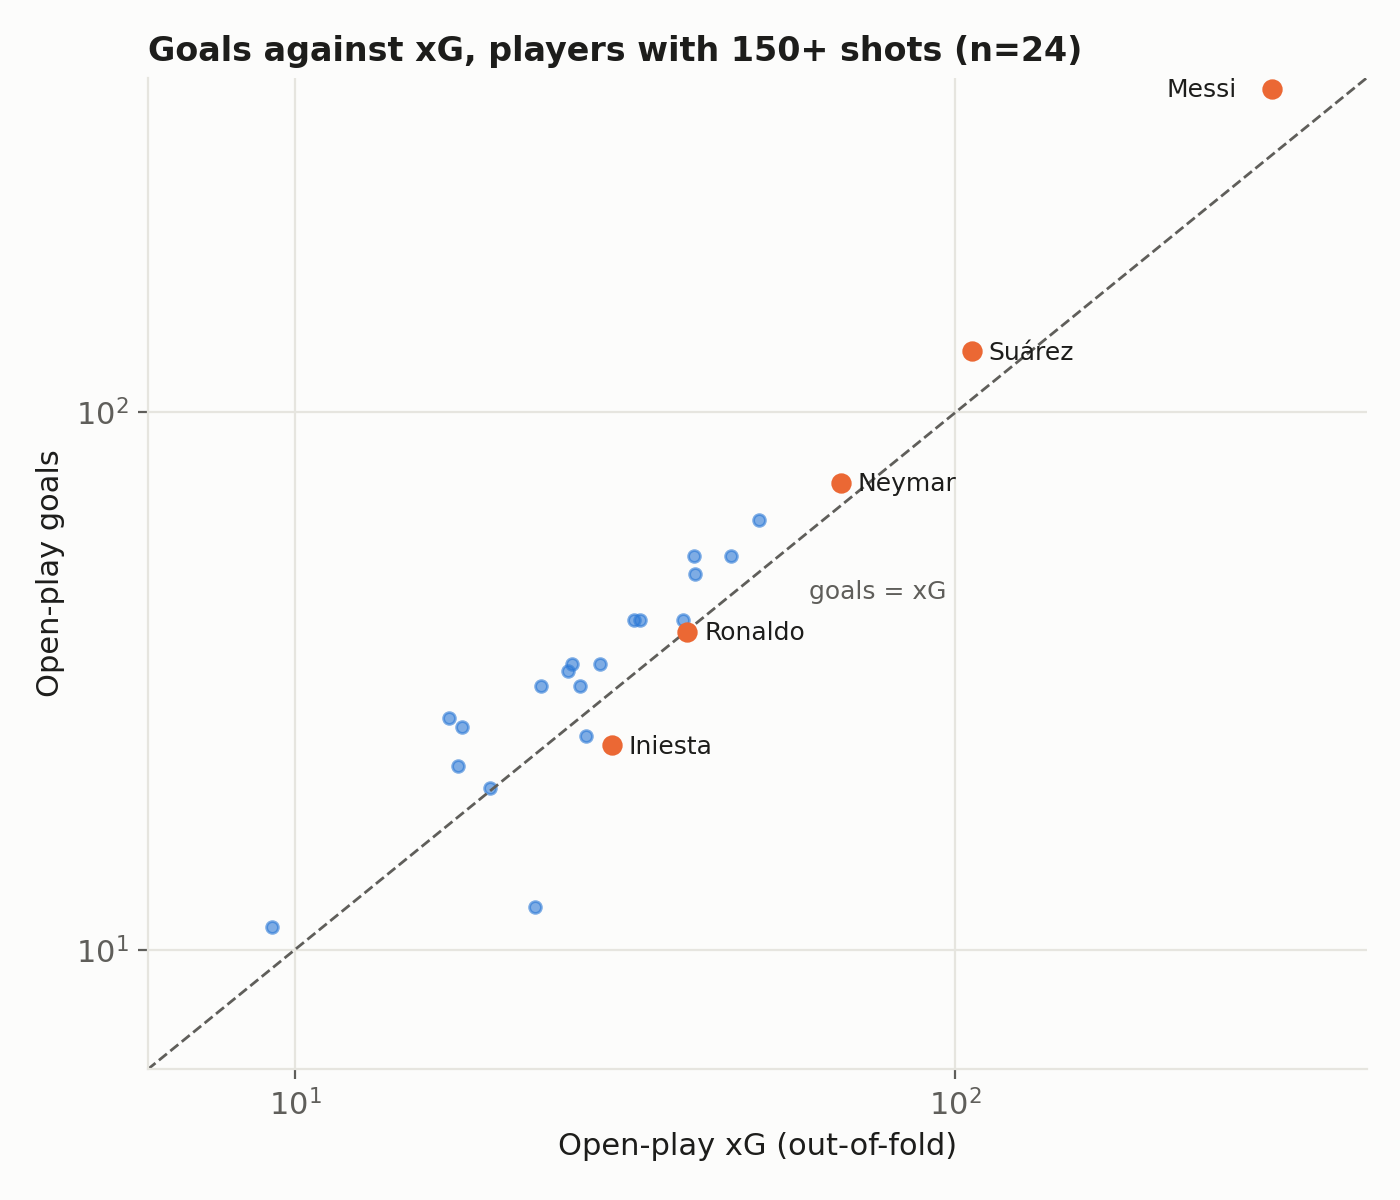
\includegraphics[width=0.75\textwidth]{images/players.png}
    \caption{Open-play Goals against xG, Players with at least 150 Shots (log scales)}
    \label{fig:players}
\end{figure}

\begin{table}[!h]
\centering
\begin{tabular}{|l|c|c|c|c|c|}
\hline
\textbf{Player} & \textbf{Shots} & \textbf{Goals} & \textbf{xG} & \textbf{Goals $-$ xG} & \textbf{$z$} \\
\hline
Lionel Messi & 2,107 & 400 & 301.2 & +98.8 & +6.8 \\
Luis Suárez & 601 & 130 & 106.0 & +24.0 & +2.9 \\
Kylian Mbappé & 288 & 54 & 40.2 & +13.8 & +2.6 \\
Samuel Eto'o & 295 & 63 & 50.4 & +12.6 & +2.2 \\
Neymar & 407 & 74 & 67.2 & +6.8 & +1.0 \\
Cristiano Ronaldo & 320 & 39 & 39.3 & $-$0.3 & $-$0.1 \\
Andrés Iniesta & 367 & 24 & 30.2 & $-$6.2 & $-$1.3 \\
Martin Braithwaite & 156 & 12 & 23.1 & $-$11.1 & $-$2.8 \\
\hline
\end{tabular}
\caption{Open-play finishing of selected players with at least 150 shots in the open data}
\label{tab:finishing}
\end{table}

\textbf{Lionel Messi} is the outstanding finisher in the data (figure \ref{fig:players} and table \ref{tab:finishing}). From 2,107 open-play shots he scored 400 goals against 301.2 xG, almost 99 goals more than an average finisher would have scored from the same chances, and a $z$ score of +6.8 rules out luck. Luis Suárez (+24.0, $z$ = +2.9) and Kylian Mbappé (+13.8, $z$ = +2.6) also clearly beat their xG. Neymar scored slightly more than his xG, within what luck could explain.

\textbf{Andrés Iniesta} scored 24 goals from 367 shots, 6.2 fewer than his xG ($z$ = $-$1.3, within the range of luck). The bigger reason for his low tally is the chances themselves: his average shot was worth 0.082 xG, against 0.103 for all shots in the data. Iniesta mostly shot from positions where goals are unlikely, which fits a playmaker who created chances for others.

The coverage of the open data should be kept in mind: Barcelona's players appear in every Barcelona La Liga match from 2004/05 to 2020/21, while most other players appear only in the competitions and seasons the open data covers. Cristiano Ronaldo's 320 shots, for example, cover only a small part of his career.

\subsection{Barcelona}

The same finishing quality shows at team level. Barcelona scored more open-play goals than their xG in 15 of the 17 La Liga seasons in the data (figure \ref{fig:barca}), with the peak in 2012/13: 85 goals from chances worth 51.6 xG. On Barcelona's shots in the test matches, the model predicts 15\% fewer goals than they scored, while it predicts the goals of all other teams within 1\%.

\begin{figure}[!h]
    \centering
    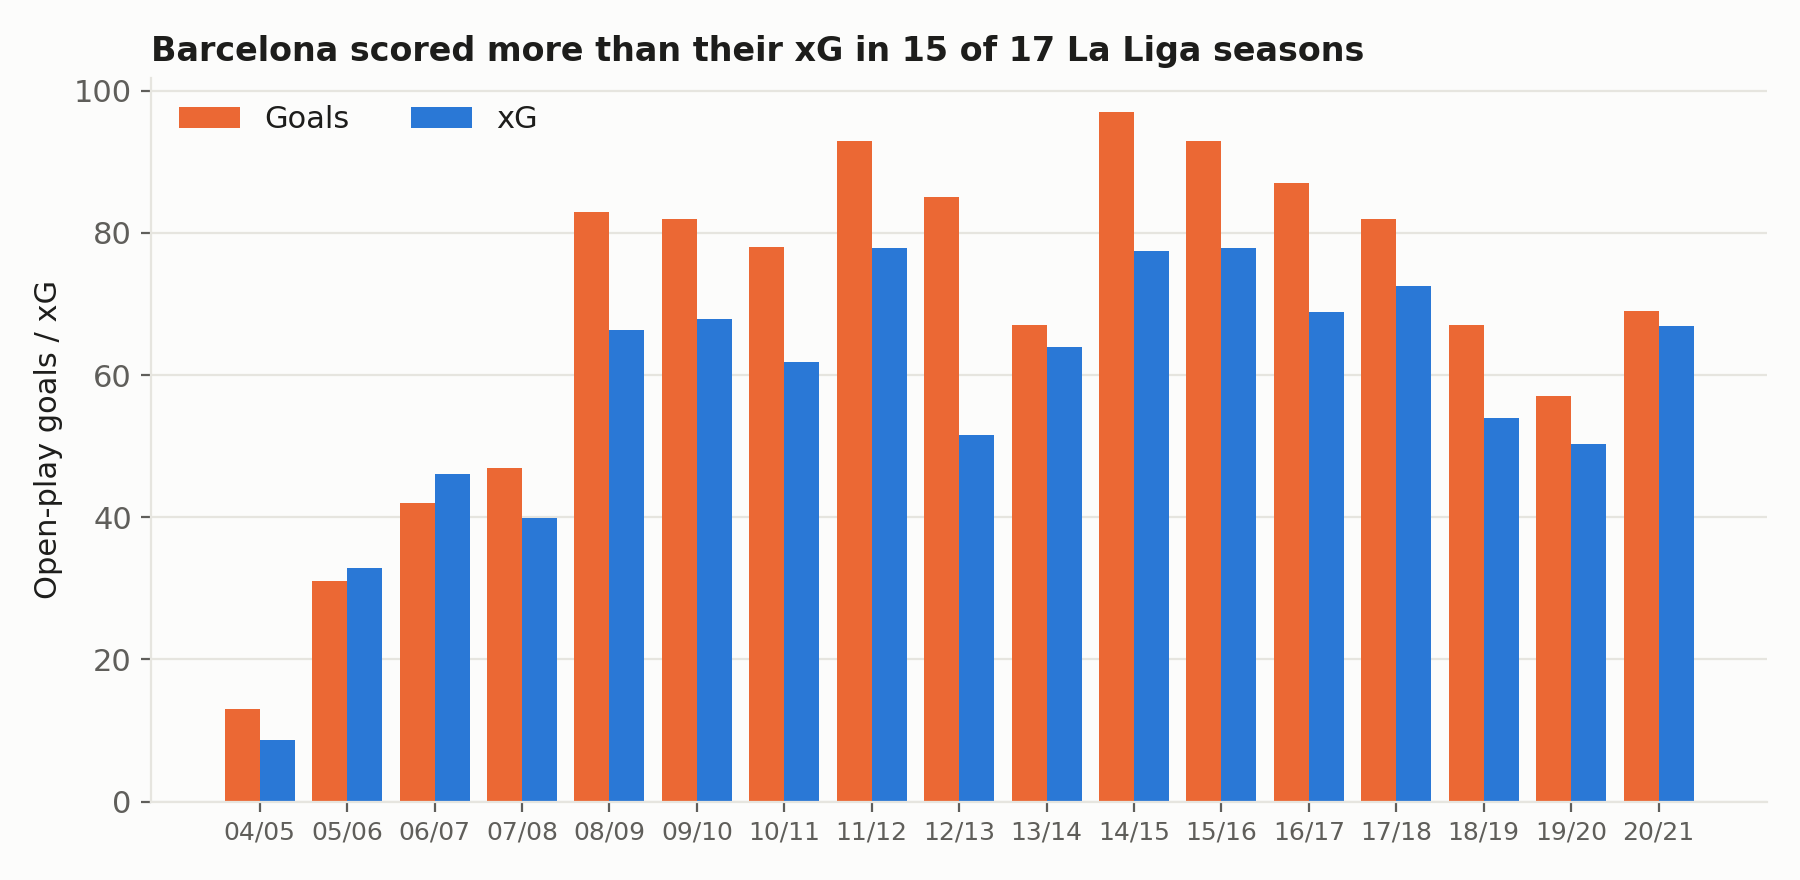
\includegraphics[width=0.9\textwidth]{images/barcelona_seasons.png}
    \caption{Barcelona in La Liga: Open-play Goals and xG by Season}
    \label{fig:barca}
\end{figure}

\newpage

\section{One Model for Different Leagues?}\label{res:leagues}

Each league has its own style of play, which raises the question whether a model trained on several leagues is biased for each of them. This was tested on the four complete 2015/16 seasons: 35,645 open-play shots from 1,517 matches. The matches of each league were split into 5 folds, and every held-out fold was predicted by models trained in four ways:
\begin{itemize}
    \item \textbf{Pooled}: trained on all four leagues
    \item \textbf{Own league only}: a separate model for each league
    \item \textbf{Other three only}: trained without the league being predicted, a direct test of whether a model transfers between styles
    \item \textbf{Pooled with a league feature}: told which league each shot is from, so it can learn an adjustment for each league
\end{itemize}

CatBoost and Logistic Regression were used, with the settings tuned in section \ref{res:models}. The 95\% intervals come from resampling whole matches.

\begin{table}[!h]
\centering
\resizebox{\textwidth}{!}{%
\begin{tabular}{|l|c|c|c|c|c|}
\hline
\textbf{League} & \textbf{Pooled} & \textbf{Own league} & \textbf{Other three} & \textbf{League feature} & \textbf{StatsBomb} \\
\hline
Premier League & 1.03 (0.96--1.10) & 0.98 (0.92--1.05) & 1.04 (0.97--1.11) & 1.01 (0.94--1.08) & 1.00 (0.93--1.07) \\
La Liga & 0.99 (0.93--1.04) & 0.98 (0.93--1.04) & 0.99 (0.93--1.04) & 0.99 (0.94--1.05) & 0.97 (0.91--1.02) \\
Serie A & 0.99 (0.93--1.05) & 0.98 (0.92--1.04) & 0.99 (0.93--1.05) & 0.99 (0.93--1.05) & 0.98 (0.93--1.04) \\
Ligue 1 & 0.98 (0.92--1.04) & 0.98 (0.92--1.05) & 0.97 (0.91--1.04) & 0.98 (0.92--1.05) & 0.96 (0.90--1.02) \\
\hline
\end{tabular}}
\caption{Predicted ÷ actual goals per league, CatBoost, with 95\% intervals}
\label{tab:leaguecal}
\end{table}

\begin{figure}[!h]
    \centering
    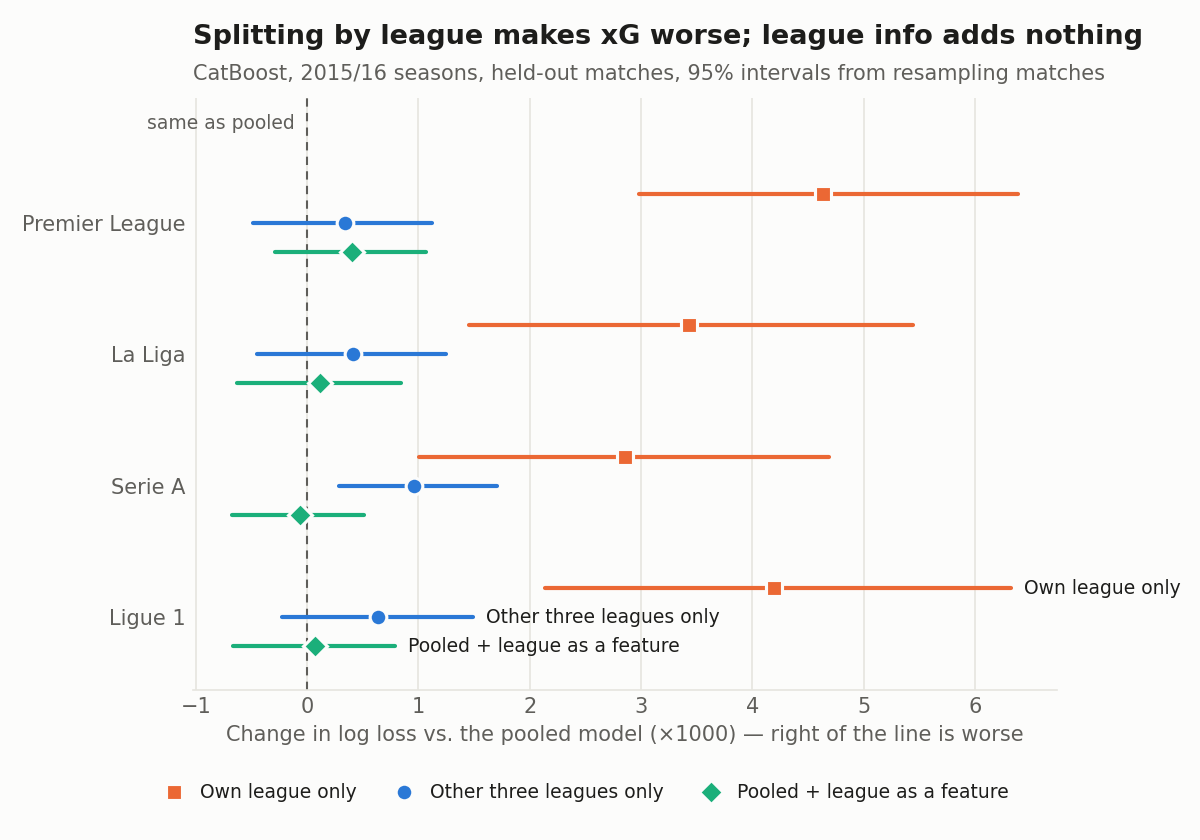
\includegraphics[width=0.9\textwidth]{images/leagues.png}
    \caption{Change in Log Loss compared with the Pooled Model, per League}
    \label{fig:leagues}
\end{figure}

The results are clear:
\begin{enumerate}
    \item \textbf{Mixing the four leagues does not bias the model.} The pooled model is calibrated in each league (between 0.98 and 1.03 of the actual goals), and every interval includes 1.00 (table \ref{tab:leaguecal}).
    \item \textbf{A model transfers to a league it has not seen.} The model trained on the other three leagues is calibrated in all four, and its log loss is only 0.0003--0.0010 higher than the pooled model's.
    \item \textbf{Separate models per league are worse.} With CatBoost, the own-league models have a clearly higher log loss than the pooled model in all four leagues, by 0.0029 to 0.0046 (figure \ref{fig:leagues}). That is more than the whole gap between the four algorithms in section \ref{res:models}: having fewer shots to learn from costs more than specialising gains. The simpler Logistic Regression loses less from splitting, but never gains.
    \item \textbf{Telling the model the league adds nothing.} The pooled model with a league feature is indistinguishable from the pooled model in every league, for both algorithms.
\end{enumerate}

A league of a different standard is another matter. The model trained on the four European leagues predicts 12\% fewer goals than were scored in the Indian Super League 2021/22 (0.88; interval 0.80 to 0.98), and StatsBomb's own model shows the same gap (0.89). The difference there is plausibly one of finishing and goalkeeping quality rather than style, and xG for such a league should be recalibrated or used with care.

\chapter{Conclusion}

Through this study four Expected Goals (xG) models were built, with the following aims:
\begin{itemize}
    \item Measure the quality of chances created by footballers and footballing teams
    \item Highlight the use of xG in player profiling and match strategy
    \item Introduce how AI based on probability is used in football
    \item Establish a bedrock for future metrics
    \item Test whether one xG model can serve different leagues and styles of play
\end{itemize}

The models were trained on 61,003 open-play shots from 2,616 men's matches in StatsBomb's open data, and tested on 524 matches they had never seen. This study includes features that some earlier studies (section \ref{lit}) did not, notably the position of the goalkeeper and the number of players between the ball and the goal, which the model in \cite{rathke2017examination} did not consider.

\section{The Models}

The main conclusions about the models are:
\begin{itemize}
    \item \textbf{All four models are well calibrated.} Logistic Regression, XGBoost, LightGBM and CatBoost all predict within 1.5\% of the goals actually scored in the test matches, with a calibration error of about half a percentage point. Their xG values can therefore be added up to judge players and teams.
    \item \textbf{The algorithm matters little.} The four models are almost tied (log loss 0.2686--0.2699, AUC 0.804--0.806). CatBoost had the best cross-validated log loss and was chosen as the final model, but its advantage over the far simpler Logistic Regression is within what chance could explain. Earlier studies such as \cite{anzer2021goal} and \cite{madrero2020creating} found XGBoost to perform best; in this study the boosting models were indistinguishable from one another and only marginally better than Logistic Regression. Logistic Regression, which is the easiest to interpret, remains a strong choice for an xG model.
    \item \textbf{The geometry of the shot matters most.} Both Logistic Regression and CatBoost rely above all on shot distance and shot angle, followed by the number of players between the ball and the goal, the goalkeeper's position and the body part. Pressure and pass type add a little, and the play pattern, grouped into Regular and Non Regular Play, adds nothing.
    \item \textbf{Comparing at the same distance matters.} In the exploratory analysis, body part, pressure and pass type barely relate to goals when taken over all distances, because headers, pressured shots and shots after high passes are all taken closer to goal. Within the same distance, a header, a shot under pressure and a shot after a high pass are all clearly worse chances. Distance has to be accounted for before such features are judged.
    \item \textbf{StatsBomb's xG remains slightly better at ranking chances} (AUC 0.813), as expected from a model trained on far more data and information, but on these matches it was less well calibrated, predicting 6\% fewer goals than were scored.
\end{itemize}

\section{Teams and Players}

The results in chapter \ref{results} show how an xG model can be used to profile teams and players:
\begin{itemize}
    \item Over a season, a team's xG difference tracks its points closely (rank correlation 0.73--0.85 in the three complete 2015/16 leagues), and the exceptions are informative. Leicester City won the 2015/16 Premier League while ranking only 6th on xG difference, and Arsenal, first on xG difference, finished second.
    \item Comparing goals with xG separates finishing from chance quality. Lionel Messi scored 400 open-play goals from chances worth 301 xG, almost 99 more than an average finisher would have scored, far beyond what luck could explain. Barcelona as a team scored more than their xG in 15 of 17 La Liga seasons.
    \item Andrés Iniesta scored fewer goals than his xG, but mainly because his shots were poor chances to begin with (0.082 xG per shot against an average of 0.103). His value lay in creating chances rather than taking them.
\end{itemize}

\section{Leagues and Styles of Play}

A common concern is that each league's style of play makes a model trained on several leagues biased. On the four complete 2015/16 seasons in the data, this concern was not supported. A model pooled across the Premier League, La Liga, Serie A and Ligue 1 is calibrated in each of them; a model that has never seen a league predicts it almost as well; separate models per league are clearly less accurate; and telling the model which league a shot is from adds nothing. The features describing a chance capture what matters across these styles, and more data matters more than specialising.

A league of a different standard is a different matter: the model predicts 12\% fewer goals than were scored in the Indian Super League, as does StatsBomb's model. For leagues that differ in level rather than style, xG should be recalibrated or used with care.

\section{Limitations}

\begin{itemize}
    \item StatsBomb's open data is a selection of matches, not a random sample: Barcelona's La Liga matches, the four 2015/16 leagues and a number of tournaments. Players and teams outside these are covered only partly.
    \item Only four complete league seasons are available, all from 2015/16, so changes over time or by team strength could not be studied.
    \item The model uses the 13 features of the original study. The finer play patterns, such as counter attacks, and other information available in the data were not added, so that the results stay comparable with the original edition.
\end{itemize}

\chapter{Future Work}\label{future}

\section{Improving the xG Model}
The revised analysis points to several improvements to the model itself:
\begin{itemize}
    \item \textbf{Finer play patterns.} Counter attacks convert at 16.3\%, far above any other play pattern, but the Regular/Non Regular grouping used here hides them. Keeping counter attacks, and perhaps corners, as separate categories should make the play pattern useful.
    \item \textbf{More of the freeze frame.} The model uses only two counts of opponents. The positions of the nearest defenders, whether the goalkeeper is set, and the space in front of the shooter could all be derived from the same freeze frames.
    \item \textbf{Recalibration by level.} A pooled model transfers between the top European leagues, but not fully to a league of a different standard. A simple recalibration for each such league, using its own shots, could be tested.
    \item \textbf{More seasons.} With more complete seasons, the analysis of teams and leagues could be extended to changes over time and to team strength.
\end{itemize}

\section{Beyond xG}
The work presented in this study forms a bedrock for future metrics. An important question that arises within the minds of those who actively follow xG models is\\

\begin{center}
\textit{\textbf{Why does an xG model not inculcate the shot technique used and the shot velocity?}}
\end{center}

The answer to this question serves as the provenance to a new metric. The reason why those two features are not utilized is that an xG model is a \textit{pre-shot} analysis. It simply measures a player/team's intelligence through understanding the kind of positions they get into during a football match and make the art of scoring easier. Therefore, to utilize a player's capability as a striker and a finisher, a metric to understand \textit{post-shot} analysis needs to be created. This metric is called, Expected Goals on Target (xGOT). The following points need to be considered to develop the xGOT metric

\begin{itemize}
    \item Placement of the shot
    \item Technique Used
    \item Velocity of the Shot
    \item The xG value of the Shot
\end{itemize}

A poor finisher could be hypothesised as one, who places a high xG valued shot in an easy to save position. This could be an example of how xGOT can be utilised to quantify player ability. Furthermore, xGOT can also be used to quantify the ability of the Goal Keeper saving the shot. A good Goal Keeper can be hypothesised as one who consistently saves football shots with high xGOT values.

Figure \ref{shotplace} highlights different coordinates of a goal for reference to shot placement. A good finisher can be hypothesised as one who places the shot aimed close to the four corners. Similarly a good goal keeper is one who consistently saves shots aimed at these four corners. 

\begin{figure}[!h]
    \centering
    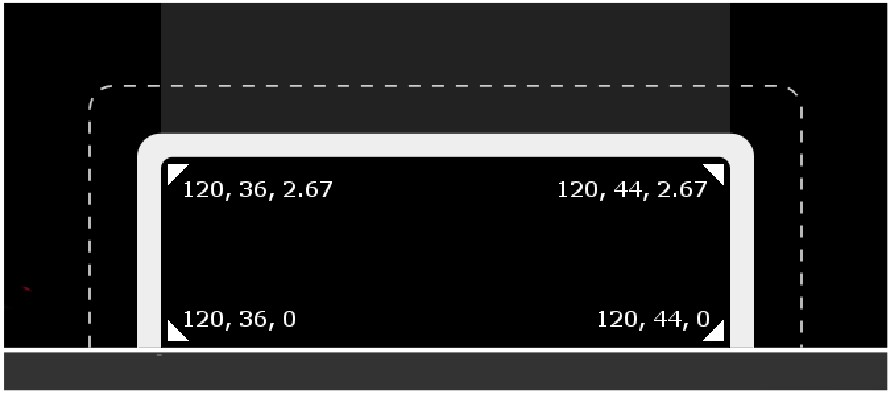
\includegraphics[scale=0.70]{images/shotplace.jpg}
    \caption{Shot Placement}
    \label{shotplace}
\end{figure}

Another metric that is derived from xG is Expected Goals Against (xGA). This metric provides perspective in how any given team allows others to create chances against themselves. A defensively good footballing team would allow others to create chances with less xG values.

A third metric that can be developed is one that analyses off-ball positioning first mentioned by author \citeauthor{spearman2018beyond} in \cite{spearman2018beyond}. This study aims at analysing the positioning of players and determining how likely they are to score while positioned without the ball highlighted in figure \ref{offball}.

\begin{figure}[!h]
    \centering
    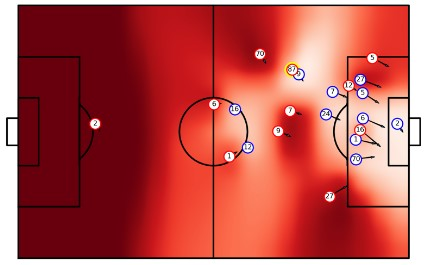
\includegraphics[scale=1, angle=90]{images/spearman.jpg}
    \caption{Off Ball Scoring}
    \label{offball}
\end{figure}





% --- project plan --- %
\chapter{Appendix A: Project Plan}
\section{Introduction}
This model was to be designed to understand Expected Goals. This chapter presents the project plan that was developed initially:
\begin{itemize}
\setlength\itemsep{-0.6em}
    \item Project Deliverables
    \item Document Conventions \& Instructions to run the Project
    \item Milestones
\end{itemize}

\section{Project Deliverable}
The following are the deliverable of the project once completed:
\begin{itemize}
\setlength\itemsep{-0.6em}
    \item Project plan
    \item Project report
    \item Power Point Presentation
    \item Poster
    \item Source Code
    \item Meeting minutes
\end{itemize}

\section{Conventions \& Instructions to run the Project}

The whole pipeline was implemented in Python. The libraries used are mentioned below:
\begin{itemize}
\setlength\itemsep{-0.6em}
    \item NumPy
    \item Pandas
    \item Beautiful Soup 
    \item Matplotlib
    \item Plotly
    \item Seaborn
    \item Sci-Kit Learn
    \item LightGBM
    \item XGBoost
    \item CatBoost
    \item SHAP
    \item Google Colab
    \item Google Drive
\end{itemize}

\subsection{Document Writing}
This report was created in latex, through the Overleaf platform.

\subsubsection{Naming Convention for Python}
Python as a programming language employs indentation to split code chunks. Nevertheless, there are some code quality standards that must be fulfilled in order to create code that is both appealing and understandable. The following steps are followed to maintain quality:
\begin{enumerate}
    \item \textbf{Imports}
    The import must be completed in a specific order. First, import the standard libraries, then third-party libraries, and ultimately local libraries. 
    \item \textbf{Indentation}
    Tab spaces are used for indentation.
    \item \textbf{Blank Spaces}
    Unnecessary blank spaces must be prevented; just one blank space must be used around each side of any operator inculcated, one following a comma, and none within the beginning or closure of parenthesis. 
\end{enumerate}

The source code was submitted via drop-off, and is not included in the report.

\subsection{Instructions for the Pipeline}

The original (2022) study used five Jupyter Notebooks, listed below. The revised edition replaces them with the \texttt{xg} Python package and command-line scripts described in Section~\ref{sec:revised-pipeline}.

The original notebooks were:

\begin{itemize}
    \item Data Extraction.ipynb
    \item Data Cleaning.ipynb
    \item EDA+Model.ipynb
    \item Pitch\_Plot.ipynb
    \item Half\_Pitch.ipynb
\end{itemize}

\subsubsection{Data Extraction}
\begin{itemize}
        \item Contains three functions
        \item Needs to be called by Data Cleaning.ipynb
        \item Fetches Competition, Match and Event Data
    \end{itemize}

\subsubsection{Data Cleaning}
\begin{itemize}
        \item Contains functions that plot freeze frames and create a DataFrame from the data obtained from Data Extraction
        \item To run it needs to be connected to the user's google drive and the necessary files must be present in the file path provided
        \item Creates a final DataFrame and pickles it for further use
    \end{itemize}

\subsubsection{EDA+Model}
\begin{itemize}
        \item Calls the pickled DataFrame and implements Exploratory Data Analysis on it
        \item Includes functions to perform feature engineering on the features
        \item Includes the final Machine Learning and Hyper-Parameter Tuning
    \end{itemize}

\subsubsection{Half\_Pitch and Pitch\_Plot}
\begin{itemize}
        \item Half\_Pitch.ipynb contains a function that allows visualisation of half a football pitch
        \item Pitch\_Plot.ipynb contains a function that allows visualisation of a football pitch
        \item Both these files should be present in the main directory and can be called from any file
    \end{itemize}

\subsection{Pipeline of the Revised Edition}
\label{sec:revised-pipeline}
{\sloppy All numbers and figures in the revised edition are produced by the code in the project repository:
\begin{itemize}
    \item \texttt{xg/data.py}: downloads and caches StatsBomb open data (competitions, matches, events)
    \item \texttt{xg/features.py}: builds the shot table and freeze-frame features from the events
    \item \texttt{xg/model.py}: modelling set, match-grouped split, model tuning and calibration metrics
    \item \texttt{xg/tables.py} and \texttt{xg/compare.py}: team and player tables, and match-bootstrap confidence intervals
    \item \texttt{scripts/}: \texttt{build\_shots.py}, \texttt{train\_evaluate.py}, \texttt{xg\_tables.py}, \texttt{league\_comparison.py}, \texttt{plot\_eda.py} and \texttt{plot\_thesis\_results.py}, run in that order
\end{itemize}
The steps are documented in \texttt{docs/DATA.md}, \texttt{RESULTS.md}, \texttt{TABLES.md} and \texttt{LEAGUES.md}.\par}

\newpage

\section{Milestones}
This section was created after the study was completed, and the table below depicts the key milestones. This table solely displays the milestones of the original 2022 study.
\begin{center}
\begin{table}[!ht]
\begin{tabular}{ |p{3.5cm}| p{8cm}|  p{2cm}|}
\hline
% head of table
\textbf{Milestone} & \textbf{Description} & \textbf{Date}\\
 % body of table
\hline
Draft Creation & Draft Literature Review Creation & 04/05/2022\\
\hline
Project Targets & Project Targets were created & 10/05/2022 \\
\hline
Data Extraction & Data was extracted successfully & 25/05/2022\\
\hline
Data Cleaning & Data Cleaning and Wrangling was carried out. & 10/06/2022\\
\hline
Data Visualisation and Exploratory Analysis & Hypothesis Testing on data was carried out and data was visualised & 18/06/2022\\
\hline
Feature Engineering & Initial features were created and Column Transformer was implemented & 24/06/2022\\
\hline
Hyperparameter Tuning and Machine Learning & Machine Learning Models were shortlisted and Hyper-parameters were tuned & 30/06/2022\\
\hline
Initial Results & Initial Results were obtained and Visualisation was initiated & 07/06/2022\\
\hline
PowerPoint Presentation & Initial results were inculcated in the presentation and the presentation was finalized & 10/06/2022\\
\hline
Further Model Tuning & Machine Learning Models were tuned further to finalize outputs & 15/06/2022\\
\hline
Report Writing and Thesis Poster & Report Writing was initiated and Points for Poster were shortlisted & 20/06/2022\\
\hline 
Report Writing and Thesis Poster & Report Writing was finalized and Thesis Poster was finalized & 13/08/2022\\
\hline
\end{tabular}
\caption{Milestones}
\label{Milestones}
\end{table}
\end{center}
% end of the FR table



%\chapter{Appendix B: Source Code}

\subsection{Half\_Pitch.ipynb}
\begin{lstlisting}[style=Python]
import matplotlib.pyplot as plt
from matplotlib.patches import Arc
import pandas as pd
def halfpitchplot():
    with plt.style.context('bmh'):
        fig = plt.figure(figsize=[15,9])
        plt.axis([50, 125, -10, 90])
        
        #plt.plot([0,0],[0,80], color="grey")
        plt.plot([60,120],[80,80], color="grey")
        plt.plot([120,120],[80,0], color="grey")
        plt.plot([120,60],[0,0], color="grey")
        plt.plot([60,60],[0,80], color="grey")

        ''' #Left Penalty Area
        plt.plot([18,18],[62,18],color="grey")
        plt.plot([0,18],[62,62],color="grey")
        plt.plot([18,0],[18,18],color="grey")

        #Left 6-yard Box
        plt.plot([0,4], [50,50],color="grey")
        plt.plot([4,4], [50,30],color="grey")
        plt.plot([4,0], [30,30],color="grey")
        '''
        
        # right penalty area
        plt.plot([120, 102], [18, 18], color='grey')
        plt.plot([102, 102], [18, 62], color='grey')
        plt.plot([102, 120], [62, 62], color='grey')

        # right six yard box
        plt.plot([120, 114], [30, 30], color='grey')
        plt.plot([114, 114], [30, 50], color='grey')
        plt.plot([114, 120], [50, 50], color='grey')


        # right goal posts
        plt.plot([120, 122], [36, 36], color='grey')
        plt.plot([120, 122], [44, 44], color='grey')
        plt.plot([122, 122], [36, 44], color='grey')

        '''# left goal posts
        plt.plot([-2, 0], [36, 36], color='grey')
        plt.plot([-2, 0], [44, 44], color='grey')
        plt.plot([-2, -2], [36, 44], color='grey')'''
        
        
        #right Arc
        rightArc = Arc((108, 40), height=18.3, width=18.3, angle=0, theta1=130, theta2=230, color='black')
        #leftArc = Arc((12,40), height=18.3, width=18.3, angle=0, theta1=310, theta2=50, color="black")
        
        #Prepare Circles
        centreCircle = plt.Circle((60,40),9.15,color="grey",fill=False)
        centreSpot = plt.Circle((60,40),0.8,color="grey")
        #leftPenSpot = plt.Circle((12,40),0.8,color="grey")
        rightPenSpot = plt.Circle((108,40),0.8,color="grey")

        #Draw Circles
        ax = plt.gca()
        ax.add_patch(centreCircle)
        ax.add_patch(centreSpot)
        #ax.add_patch(leftPenSpot)
        ax.add_patch(rightPenSpot)      
        ax.add_patch(rightArc)
        #ax.add_patch(leftArc)
        ax.set_ylim(ax.get_ylim()[::-1])
        #Tidy Axes

    
        return fig
\end{lstlisting}

\subsection{Pitch\_Plot.ipynb}
\begin{lstlisting}[style=Python]
import matplotlib.pyplot as plt
from matplotlib.patches import Arc
import pandas as pd
def pitchplot():
    with plt.style.context('bmh'):
        fig = plt.figure(figsize=[15,9])
        plt.axis([-10, 135, -10, 85])
        
        plt.plot([0,0],[0,80], color="grey")
        plt.plot([0,120],[80,80], color="grey")
        plt.plot([120,120],[80,0], color="grey")
        plt.plot([120,0],[0,0], color="grey")
        plt.plot([60,60],[0,80], color="grey")

        #Left Penalty Area
        plt.plot([18,18],[62,18],color="grey")
        plt.plot([0,18],[62,62],color="grey")
        plt.plot([18,0],[18,18],color="grey")

        #Left 6-yard Box
        plt.plot([0,4], [50,50],color="grey")
        plt.plot([4,4], [50,30],color="grey")
        plt.plot([4,0], [30,30],color="grey")

        
        # right penalty area
        plt.plot([120, 102], [18, 18], color='grey')
        plt.plot([102, 102], [18, 62], color='grey')
        plt.plot([102, 120], [62, 62], color='grey')

        # right six yard box
        plt.plot([120, 114], [30, 30], color='grey')
        plt.plot([114, 114], [30, 50], color='grey')
        plt.plot([114, 120], [50, 50], color='grey')


        # right goal posts
        plt.plot([120, 122], [36, 36], color='grey')
        plt.plot([120, 122], [44, 44], color='grey')
        plt.plot([122, 122], [36, 44], color='grey')

        # left goal posts
        plt.plot([-2, 0], [36, 36], color='grey')
        plt.plot([-2, 0], [44, 44], color='grey')
        plt.plot([-2, -2], [36, 44], color='grey')
        
        
        # right Arc
        rightArc = Arc((108, 40), height=18.3, width=18.3, angle=0, theta1=130, theta2=230, color='black')
        leftArc = Arc((12,40), height=18.3, width=18.3, angle=0, theta1=310, theta2=50, color="black")
        
        #Prepare Circles
        centreCircle = plt.Circle((60,40),9.15,color="grey",fill=False)
        centreSpot = plt.Circle((60,40),0.8,color="grey")
        leftPenSpot = plt.Circle((12,40),0.8,color="grey")
        rightPenSpot = plt.Circle((108,40),0.8,color="grey")

        #Draw Circles
        ax = plt.gca()
        ax.add_patch(centreCircle)
        ax.add_patch(centreSpot)
        ax.add_patch(leftPenSpot)
        ax.add_patch(rightPenSpot)      
        ax.add_patch(rightArc)
        ax.add_patch(leftArc)
        ax.set_ylim(ax.get_ylim()[::-1])
        #Tidy Axes

    
        return fig
\end{lstlisting}


\subsection{Data Extraction.ipynb}
\begin{lstlisting}[style=Python]
import requests
from bs4 import BeautifulSoup
import json
import re

class Game:
    """Game object whose only attribute is event-level JSON file (from Statsbomb's github)"""
    
    def __init__(self, json_file):
        self.json_file = json.loads(json_file)


def fetch_url(github_season_url):
    """
    Function which take a url from Statsbomb's github for a specific season and returns a dictionary maping game ID's to the game's 
    event level JSON data.
    
    Arguments:
    
    github_season_url - (String) URL from Statsbomb's github. Format is:
                        https://github.com/statsbomb/open-data/blob/master/data/matches/{league_ID}/{season_ID}.json
    """
    req = requests.get(github_season_url).text
    soup = BeautifulSoup(req, "lxml") 
    table = soup.find('table')
    
    game_nums = []
    for td in table.find_all('td'):
        if "match_id" in td.text:
            game_num = re.findall(r'[0-9]+', td.text)[0]
            game_nums.append(game_num)
            
    json_files = []
    base_url_string = "https://raw.githubusercontent.com/statsbomb/open-data/master/data/events/"
    game_num_dict = {
        game_num  : Game(requests.get(base_url_string + game_num + ".json").text)
        for game_num in game_nums
    }
 
    return game_num_dict


def obtain_seasons(competition_id):
    """
    Function which takes a competition_id, as specified by Statsbomb, and returns a dictionary where each season maps to 
    another dictionary containing all games in that season.
    
    Arguments:
    
    season_id - (int) competition_id as specified by Statsbomb 
                      See here: https://github.com/statsbomb/open-data/blob/master/data/competitions.json
    
    """
    #Get webpage html for competitions.json
    req = requests.get("https://raw.githubusercontent.com/statsbomb/open-data/master/data/competitions.json").text
    #Convert webpage to json format
    competitions_statsbomb = json.loads(req)

    all_seasons_id = {}
    for comps in competitions_statsbomb:
        if comps['competition_id'] == competition_id:
            season_id = comps['season_id']
            season_name = comps['season_name']
        
            all_seasons_id[season_name] = season_id
    
    league_all_games_by_seasons = {}
    
    for keys, values in all_seasons_id.items():
        season_url = "https://github.com/statsbomb/open-data/blob/master/data/matches/{}/{}.json".format(competition_id, values)
        print("Getting season {}...".format(keys))
        season = fetch_url(season_url)
        league_all_games_by_seasons[keys] = season
    
    print("Done")
    
    return league_all_games_by_seasons
\end{lstlisting}

%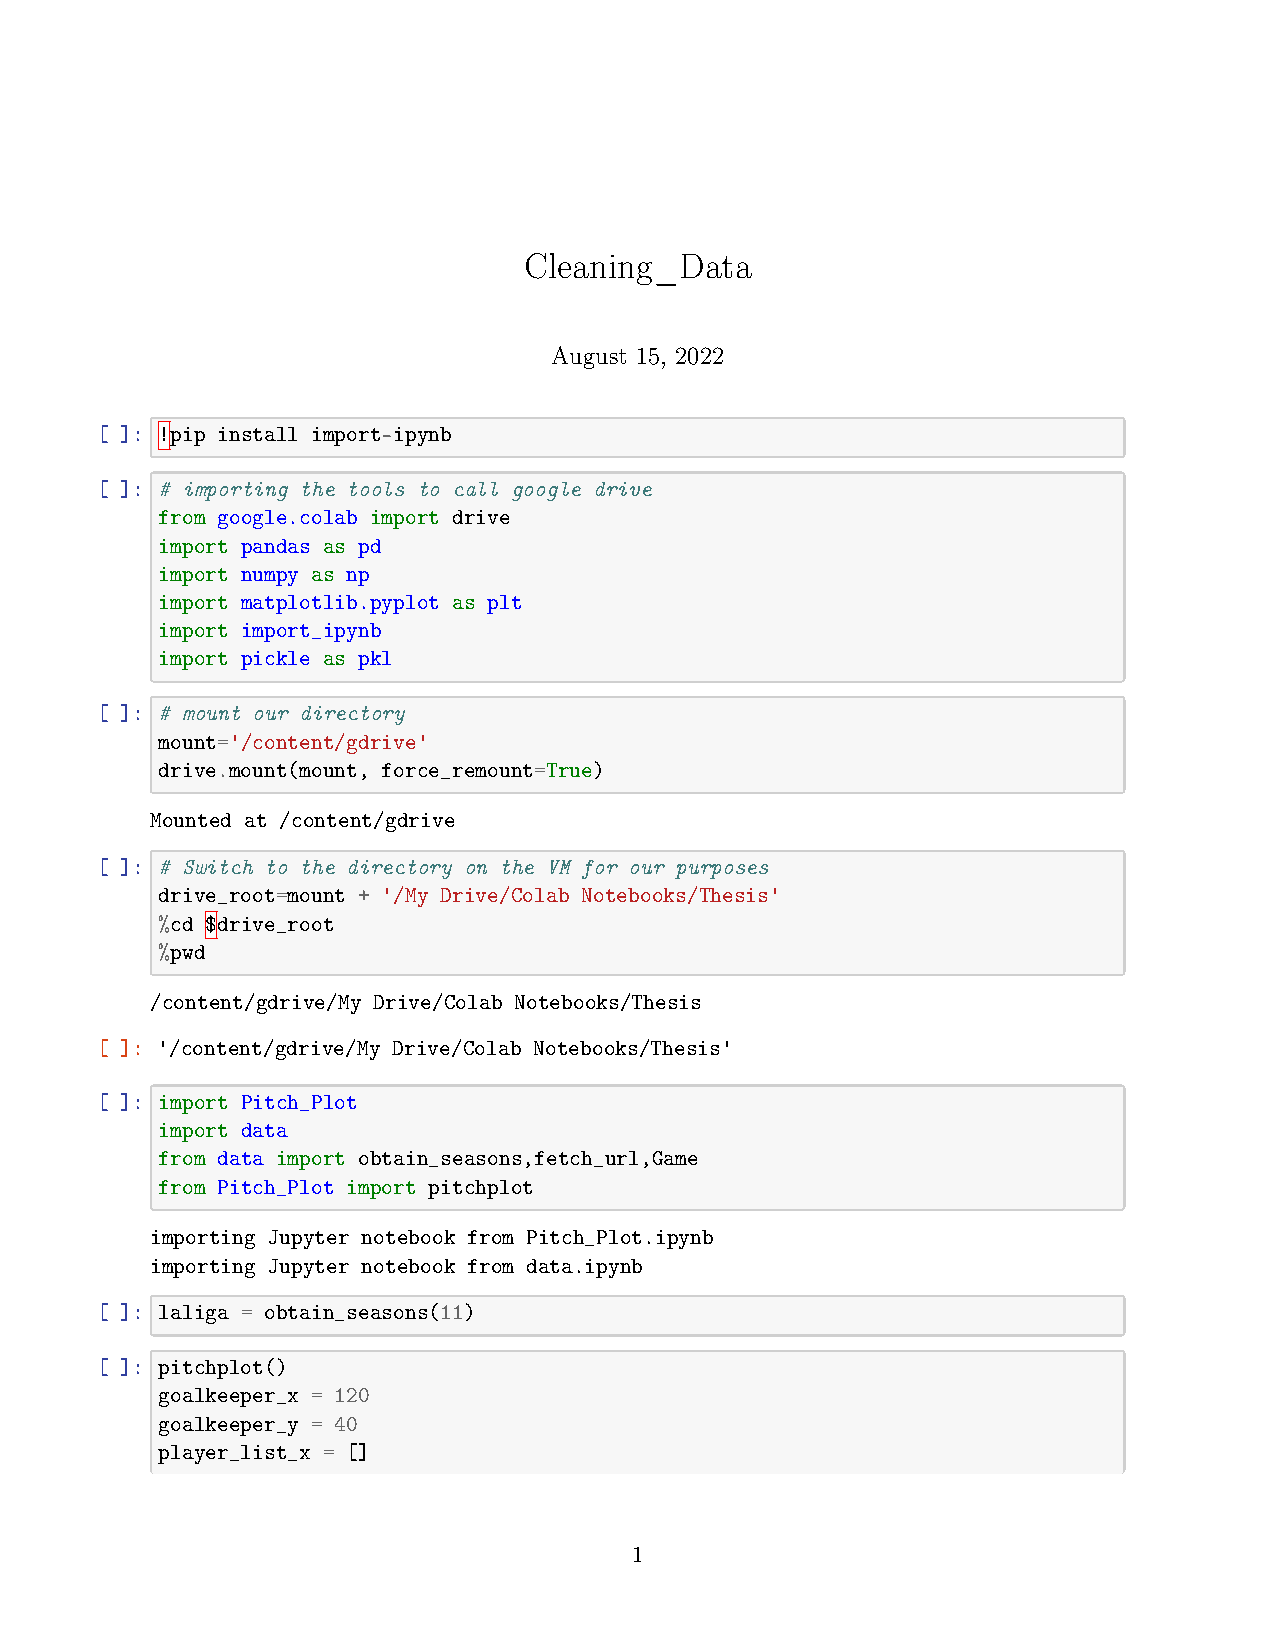
\includepdf[pages=-]{dd.pdf}
%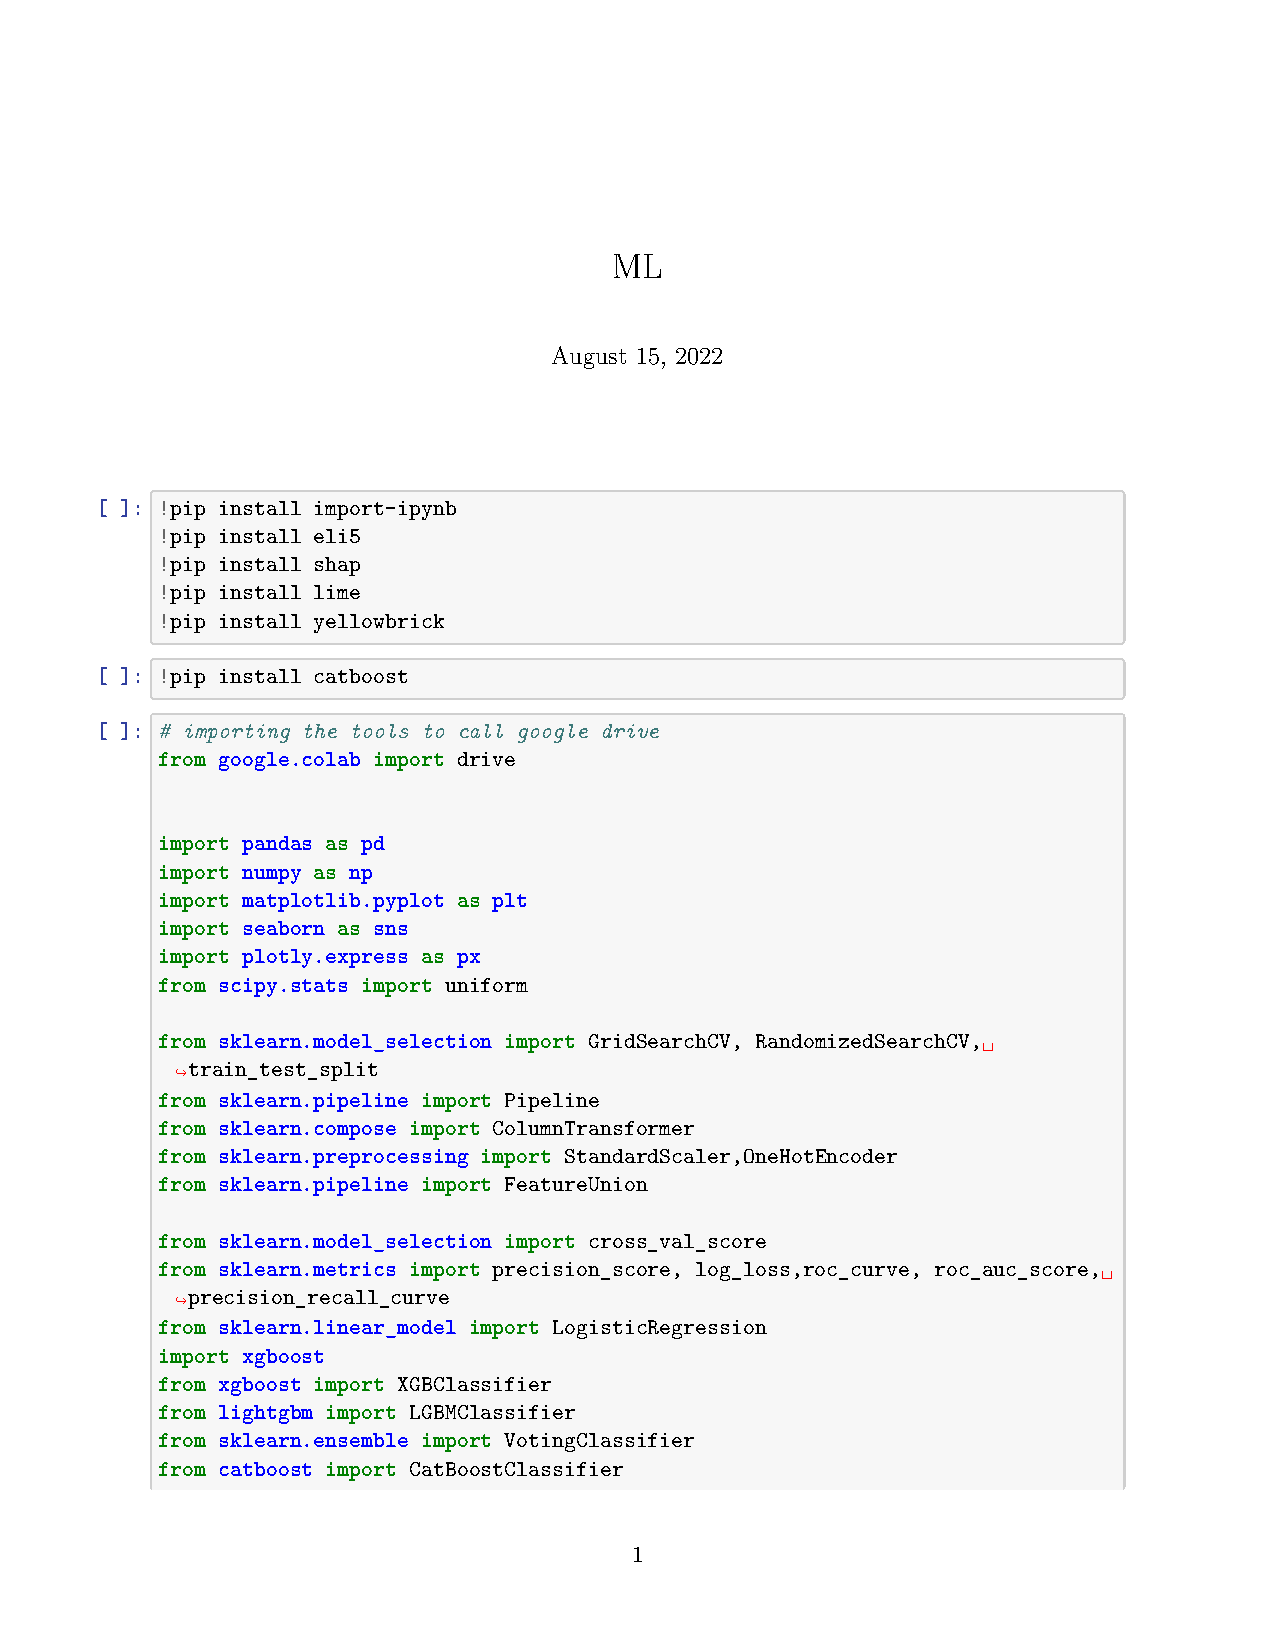
\includepdf[pages=-]{EDA+Model.pdf}
\printbibliography

\end{document}